\documentclass[11pt,a4paper,titlepage]{scrartcl}

\usepackage{harvard}
%notwendiges Package f\"ur Journal of Finance Bibliostyle
%\usepackage{babelbib}
\usepackage{graphicx}
\usepackage{setspace}
\usepackage[english]{babel}
\usepackage{amsmath}
%\usepackage{times}
\usepackage{booktabs}
\usepackage[utf8]{inputenc}

\usepackage{geometry}
\geometry{a4paper, top=30mm, left=30mm, right=30mm, bottom=30mm}




%kann angeschaltet werden, falls Times Schrift erw\"unscht
\usepackage{array}
\usepackage{tabularx}
\usepackage{dcolumn}
\usepackage{longtable}
\usepackage{colortbl}
\usepackage{rotating}
\usepackage{multirow}
\usepackage{scrlayer-scrpage}
\usepackage{nameref}
\usepackage{amsfonts}


\usepackage{txfonts} %Schriftart Times New Roman
\usepackage{ulem} %added by me
\usepackage{caption}  % added by me for text in table
\usepackage{placeins} %added by me Include this for \FloatBarrier
\usepackage{float} % Added by me to 'fix' tables
\usepackage{listings}% Added by me to render formatting


\usepackage[colorlinks=true, linkcolor=black, citecolor=black, urlcolor=black]{hyperref} % Include this in the preamble for \url{}. must be after all the usepackage

%\usepackage{hyperref} %


\pagestyle{scrheadings} 
\clearpairofpagestyles
\rohead{\headmark}                                   

 

\linespread{1.5}
%Stellt Zeilenabstand ein
\setlength{\footheight}{20.40001pt} 
\setlength{\headheight}{20.40001pt}

%BEGIN DOCUMENT%%%%%%%%%%%%%%%%%%%%%%%%%%%%%%%%%%%%%%%%%%%%%%%%%%

\begin{document} 


\newpage

\thispagestyle{plain}
\begin{titlepage}

\begin{center}

\huge{\textbf{Flash loans in ethereum using Aave}}\\[1.5ex]
\LARGE{Different use cases with specific analysis of applications}\\[6ex]
\Large{Advanced Studies in Finance /  Finance Master Thesis \\
Finance Executive Education  \\
Finance Weiterbildung}\\[1.5ex]
\Large{Dr. Benjamin Wildiing}\\
\Large{Manuel Keller}\\[12	ex]


\end{center}


\normalsize
\begin{flushleft}
Written by:\\[3ex]
Andrea Merli\\[1ex]
Plattenstrasse 14\\[1ex]
8302 Zürich\\[3ex]

Filling date: XX.Januar.20YY\\[10ex]
\end{flushleft}

\begin {figure}[h]
\begin {center}

\includegraphics [width=4.5cm] {uzh_logo_d_pos.eps}
\end {center}
\end {figure}


\end{titlepage}


%Der folgende Abschnitt erm\"oglicht das einf\"ugen von der eingescannten Aufgabenstellung (hier drei Seiten) Scale und Ordnerangabe (Zusatz/AuftragX) muss an die jeweiligen Bed\"urfnisse angepasst werden.
%\markboth{}{Aufgabenstellung}
%\cfoot{}
%\begin{center}
%\includegraphics[scale=0.73]{Zusatz/Auftrag1}

%\includegraphics[scale=0.73]{Zusatz/Auftrag2}

%\includegraphics[scale=0.73]{Zusatz/Auftrag3}

%\end{center}
\pagenumbering{Roman}
\cfoot{\pagemark}
\newpage
%\pagenumbering{Roman}
\section*{Abstract}
\normalsize
abstract abstract abstract abstract abstract abstract abstract abstract abstract abstract abstract abstract abstract abstract abstract abstract abstract abstract abstract abstract abstract abstract abstract abstract abstract abstract abstract abstract abstract abstract abstract abstract abstract abstract abstract abstract. abstract abstract abstract abstract abstract abstract abstract abstract abstract abstract abstract abstract abstract abstract abstract abstract abstract abstract abstract abstract abstract abstract abstract abstract abstract abstract abstract abstract abstract abstract abstract abstract abstract abstract abstract abstract abstract abstract abstract abstract abstract abstract abstract abstract abstract abstract abstract abstract abstract abstract abstract abstract abstract abstract abstract abstract abstract abstract abstract abstract abstract abstract abstract abstract abstract abstract abstract abstract abstract .

\newpage





\tableofcontents

\newpage

\listoffigures

\newpage

\listoftables

\newpage
\section*{Abbreviations}

\newpage

\pagenumbering{arabic}

%%%%%%%%%%%%%%%%%%%%%%%%%%% EINLEITUNG
\section{Einleitung \label{sect:Introduction}}
\subsection{Ausgangslage und Problemstellung}
\subsection{Ziel der Arbeit}
\subsection{Aufbau und Vorgehen}
\subsection{Abgrenzungen}

\newpage

\section{Aave protocol}
\subsection{Aave lending protocol basics}
Aave is one of the most used and battle tested lending protocols in DeFi. Before Aave version 1 (V1) there were other solutions for decentralised lending strategy, among them, ethlend which has been founded by the same team and it is the natural Aave precursor; ethlend was  peer to peer (P2P), resulting in a direct lender - borrower matching handled by a smart contract. A traditional finance instrument to represent this is an OTC contract, represented in figure \ref{fig:peer_lending} to which the decentralized finance (DEFI) community added, at first, a layer for decentralisation and peers matching. The P2P approach enables  the credit process in a decentralised environment but is not flexible and is illiquid cause the charged rate and lended amount in a potential loan must be published waiting for an interested counterpart. 
\begin{figure}[ht]
    \centering
    \begin{minipage}[t]{0.45\textwidth} % Adjust width as needed
        \centering
        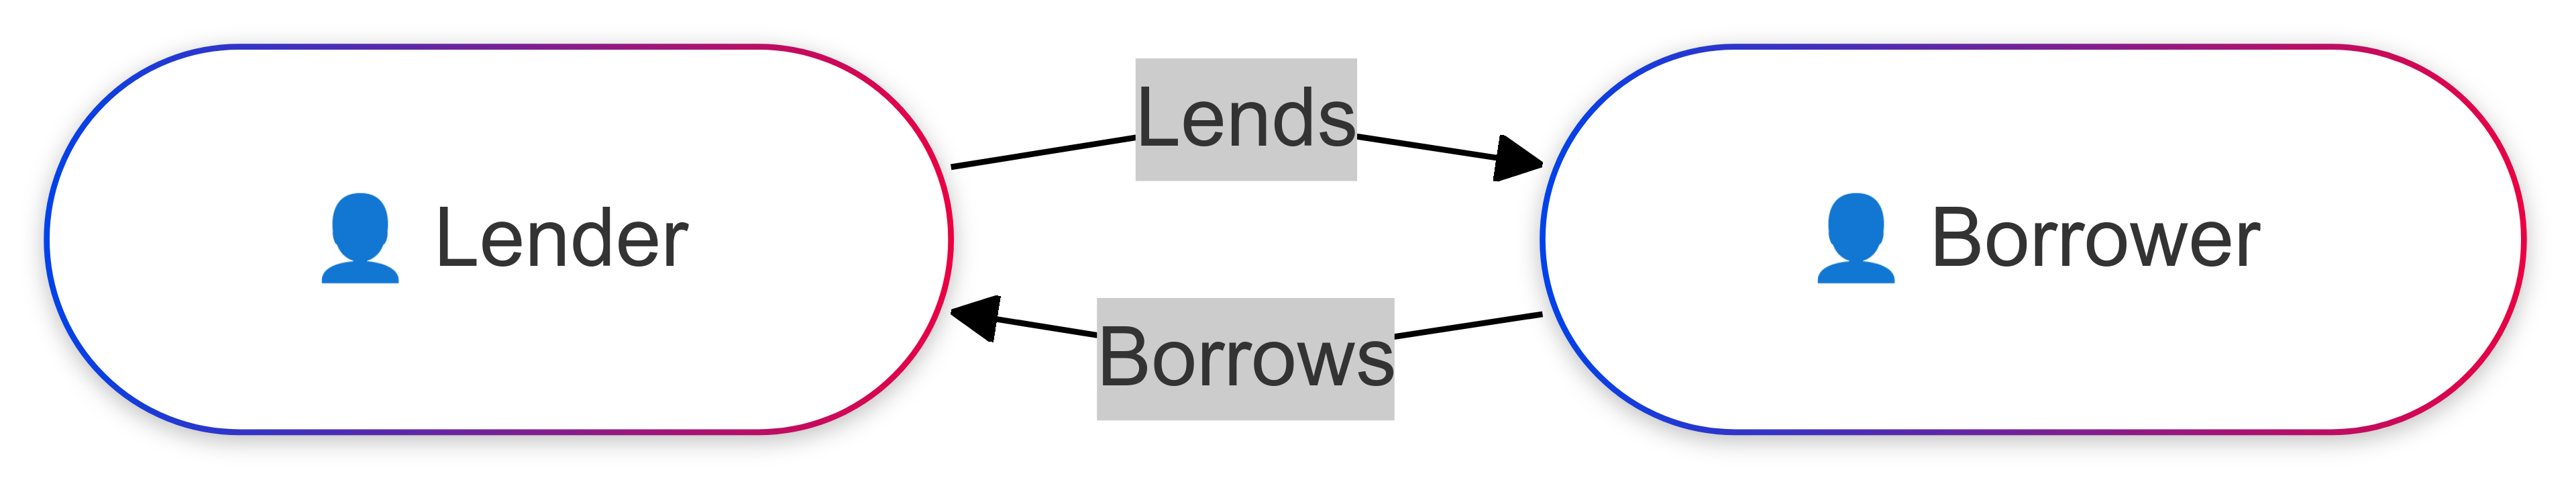
\includegraphics[width=\textwidth]{image/otclendborrow.png}
        \caption{P2P lending borrowing (OTC)}
        \label{fig:peer_lending}
    \end{minipage}
    \hfill % Horizontal space between the figures
    \begin{minipage}[t]{0.45\textwidth} % Adjust width as needed
        \centering
        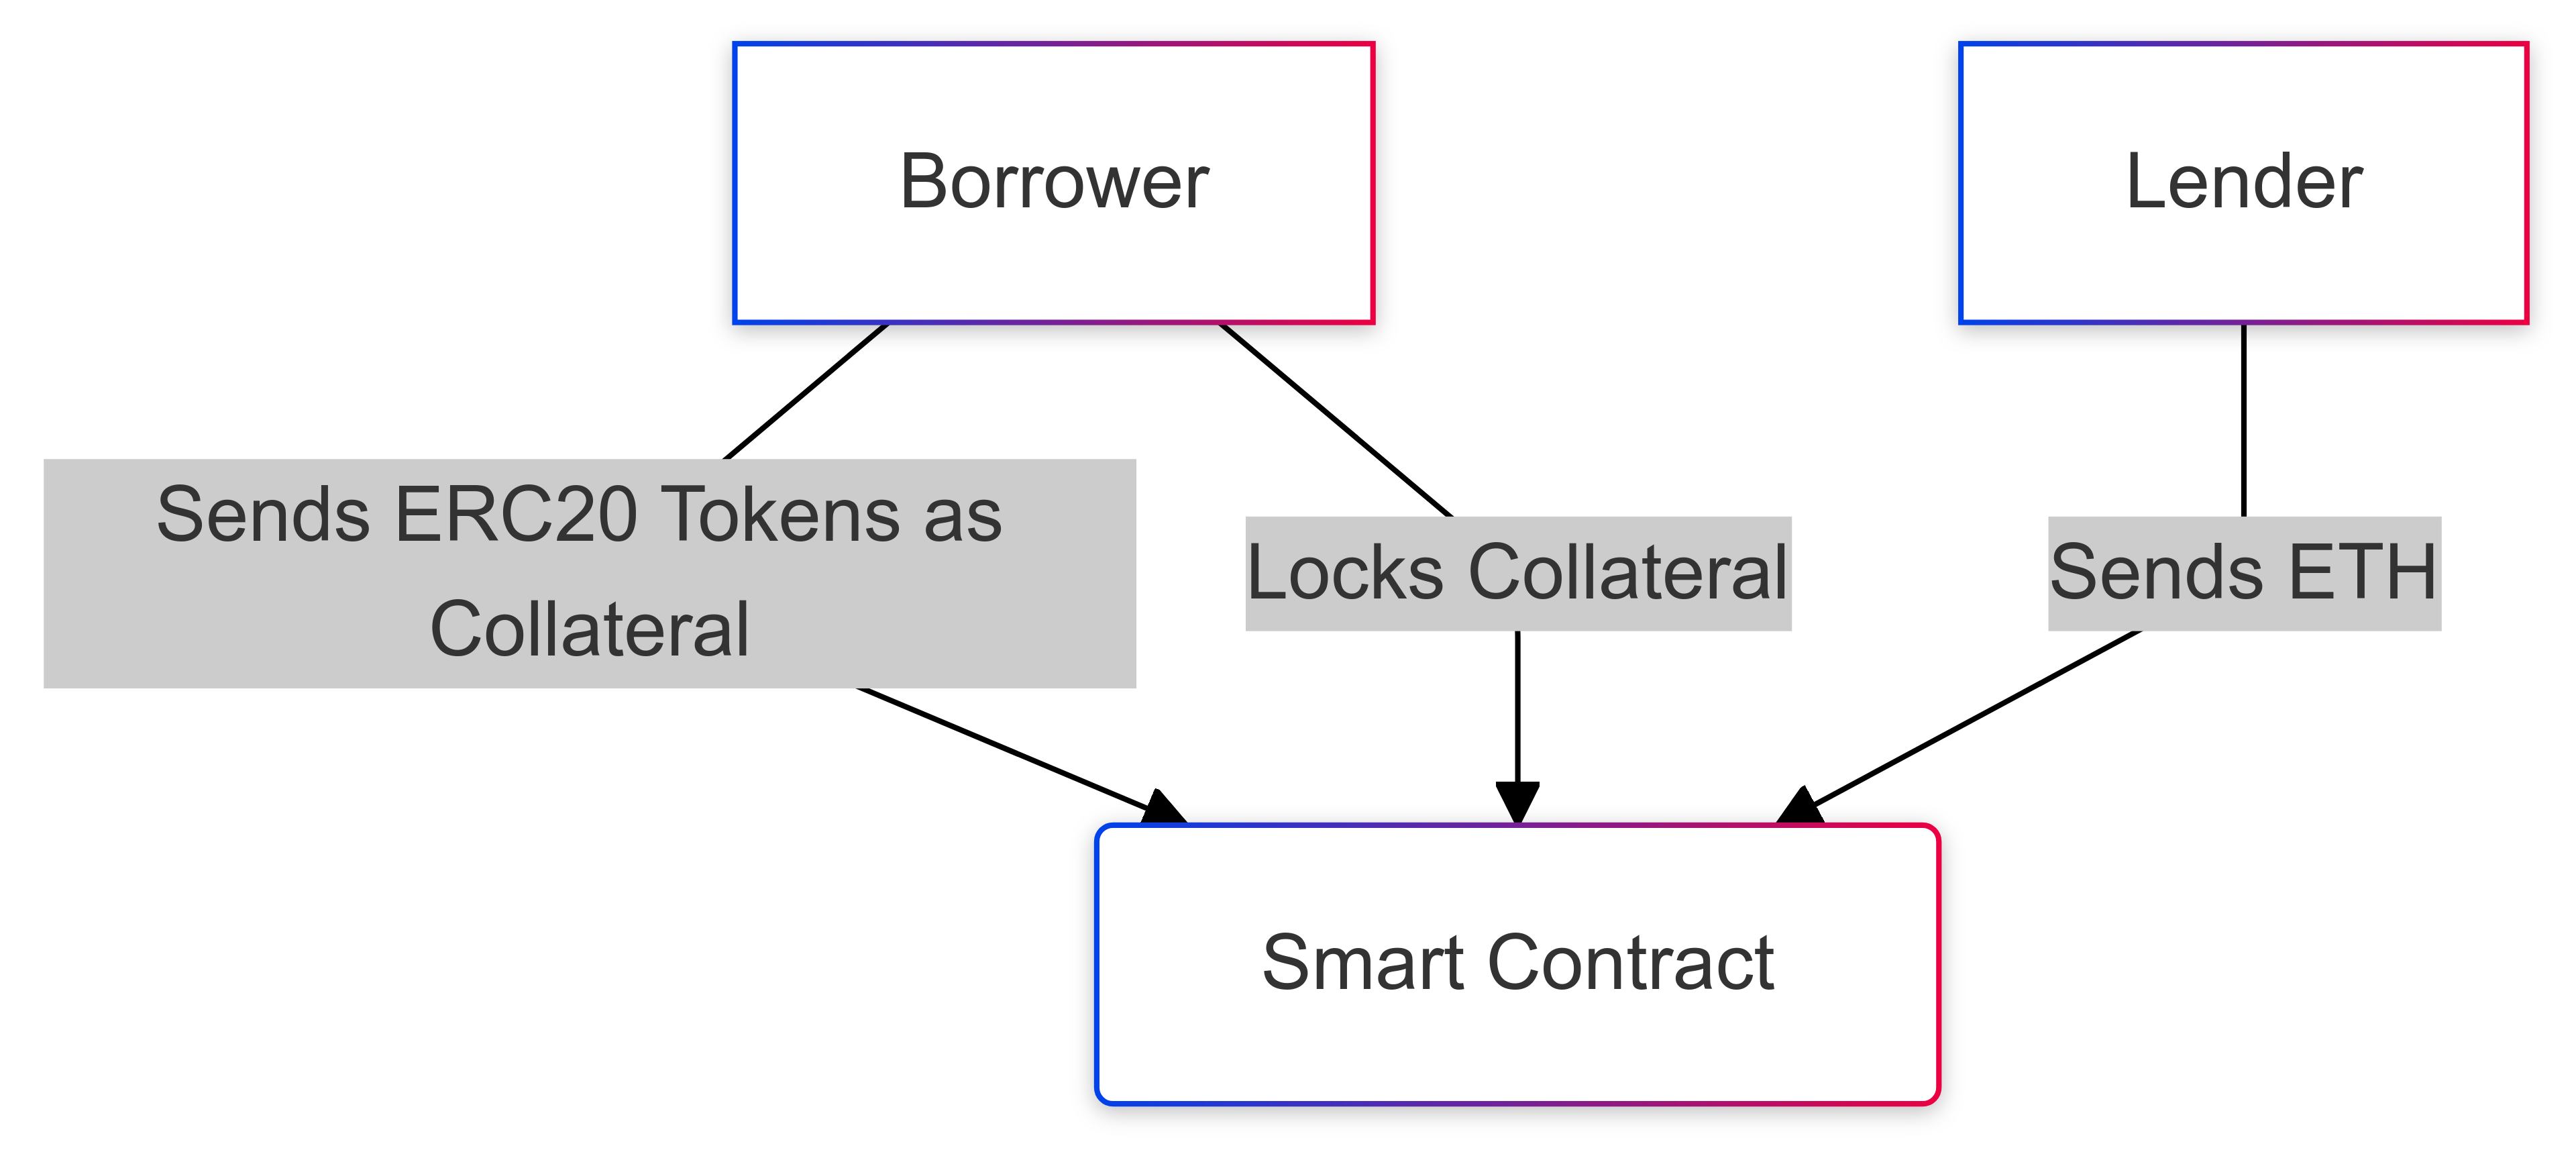
\includegraphics[width=\textwidth]{image/lenderborrowerOTC}
        \caption{smart contract handling lender borrowed P2P interaction}
        \label{fig:lending_contract}
    \end{minipage}
    \FloatBarrier
\end{figure}

In detail the OTC solution  provided by ethLend, represented in figure \ref{fig:lending_contract}, consists in a lender borrower smart contract interaction where  borrowers create a loan request  posting  ERC-20 compatible tokens  as collateral and setting  the loan’s length, interest premium and the amount of tokens needed for collateral. If a lender agrees to these terms, a loan agreement will be created.
There are only two possible outcomes: if the borrower repays the loan, the lender then receives his or her original principal plus interest and the borrower takes back the collateral which is unlocked from the smart contract whereas if the borrower fails to repay his or her loan, the lender will receive the borrower’s posted collateral. 

\begin{figure}[ht]
    \centering
    \begin{minipage}[t]{0.53\textwidth} % Adjust width as needed
        \centering
        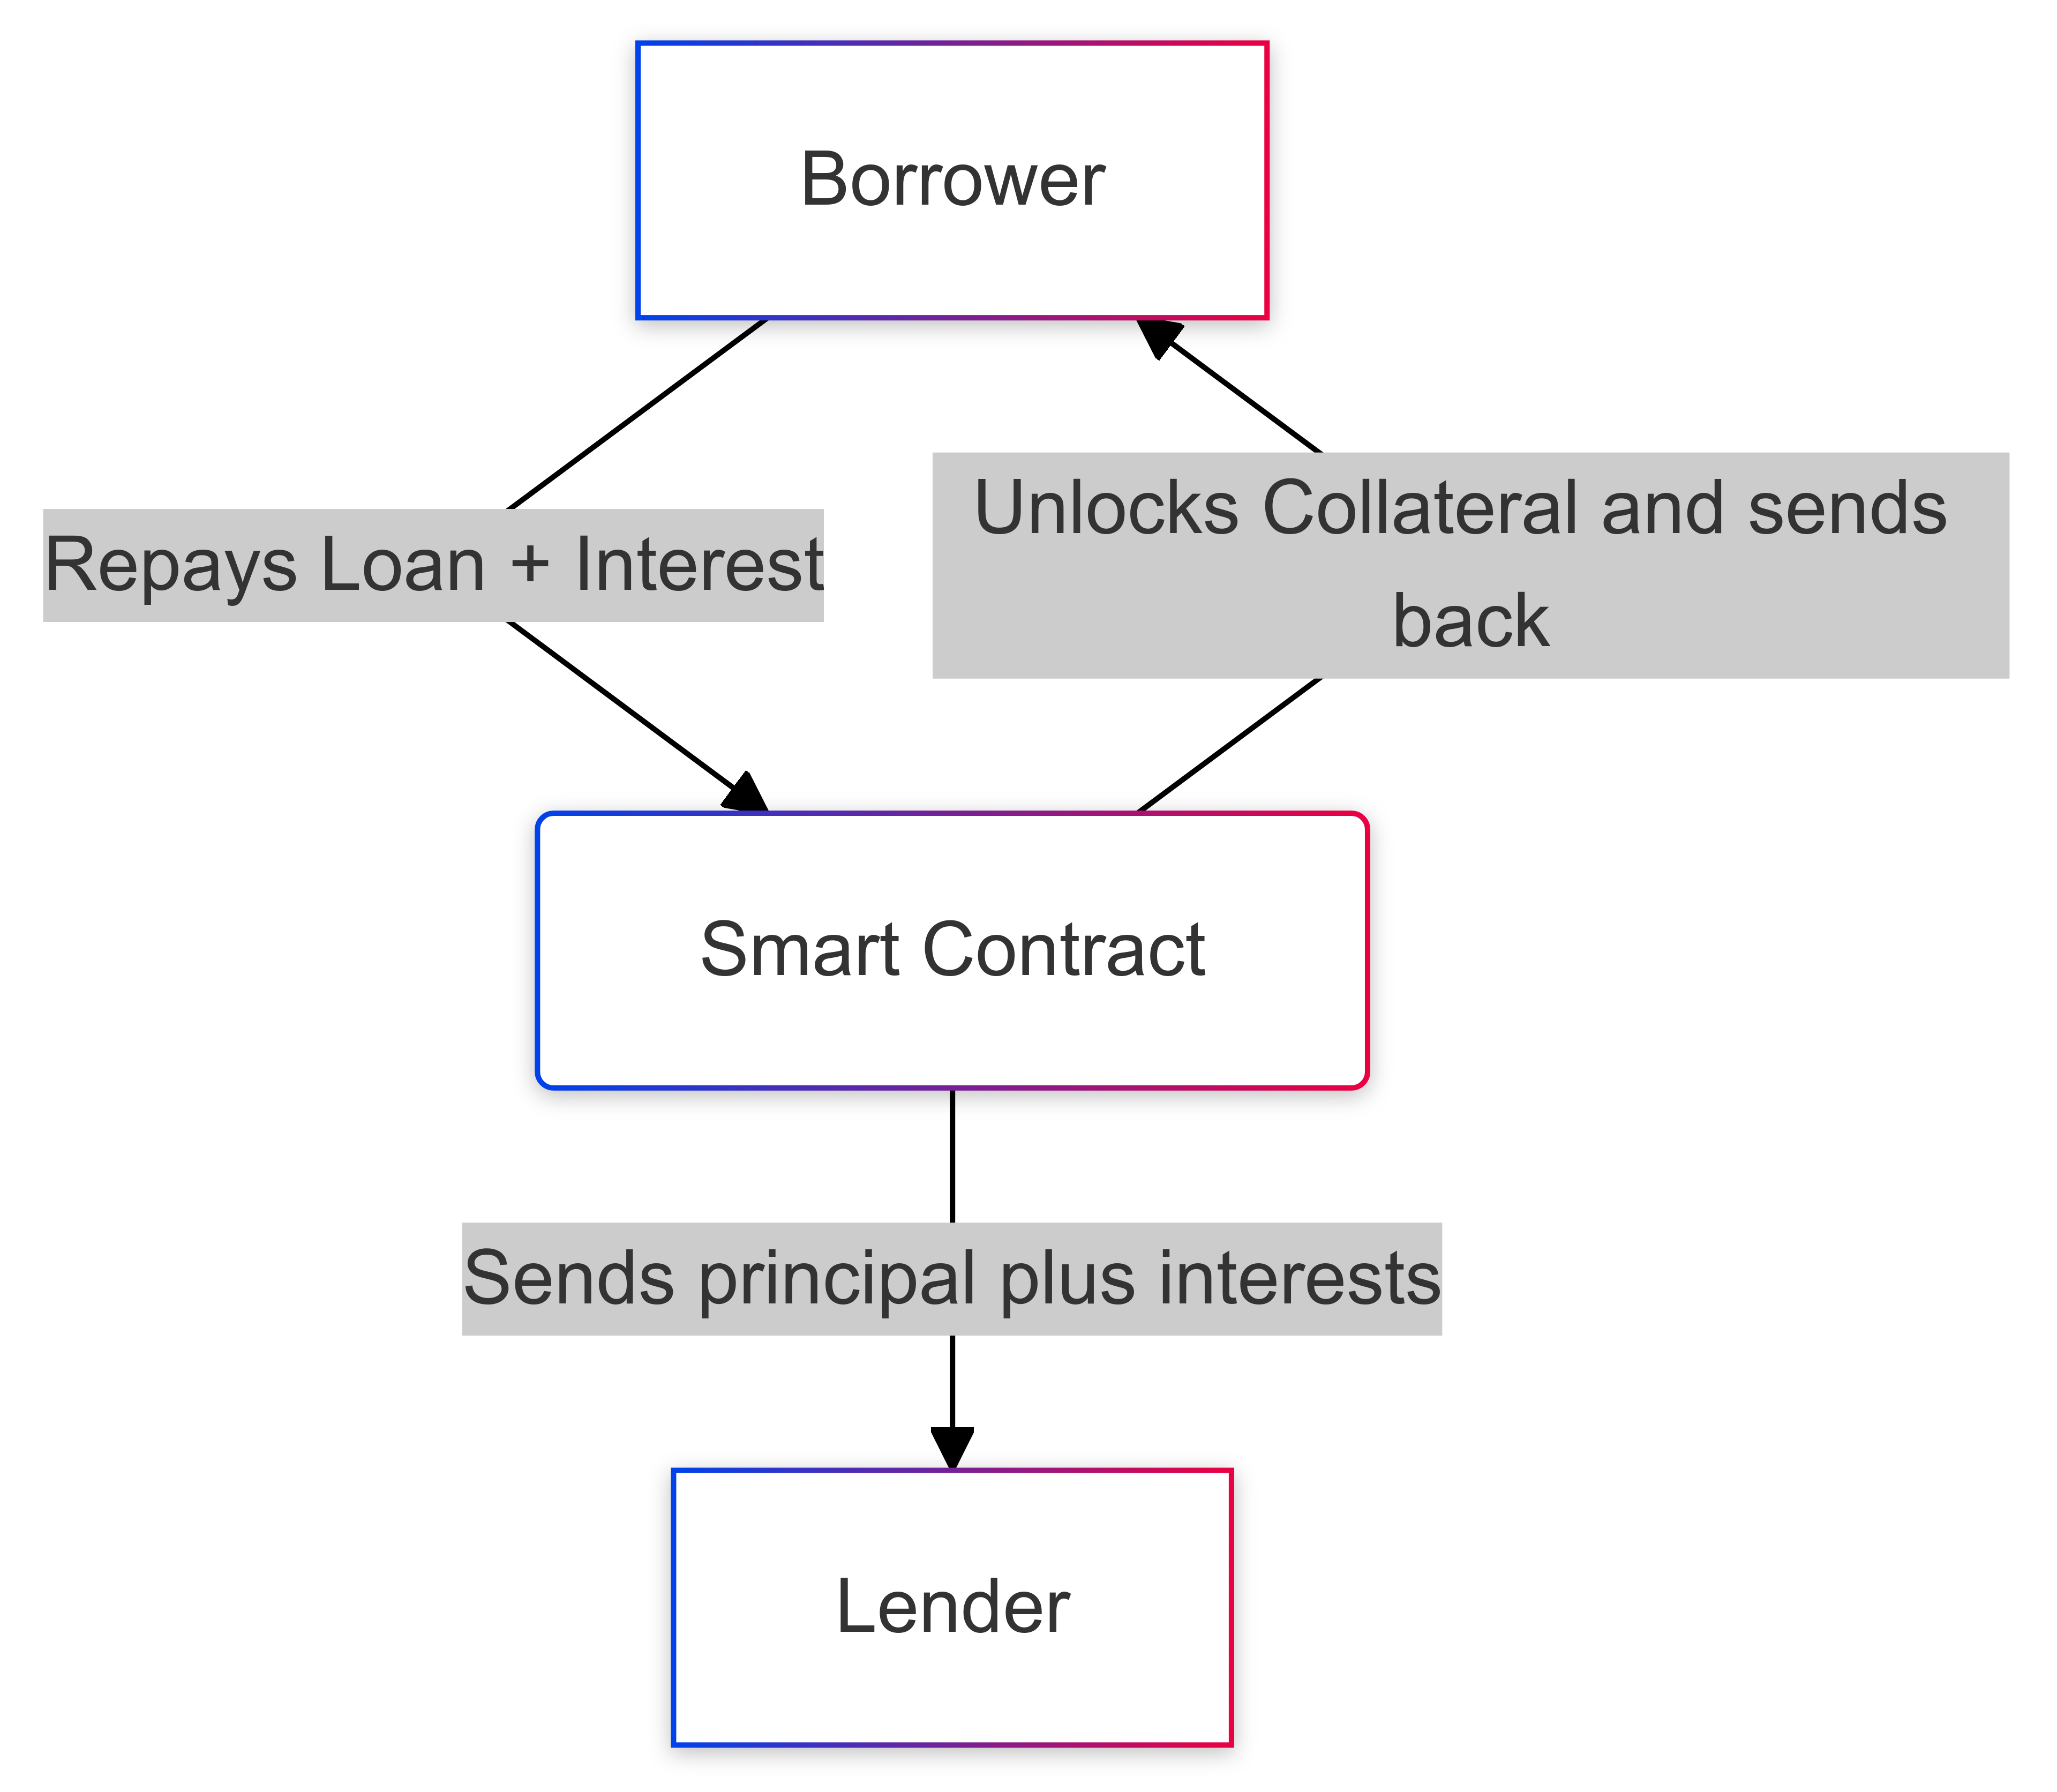
\includegraphics[width=\textwidth]{image/otcrepayment}
        \caption{Borrower repays the loan}
        \label{fig:repays}
    \end{minipage}
    \hfill % Horizontal space between the figures
    \begin{minipage}[t]{0.3\textwidth} % Adjust width as needed
        \centering
        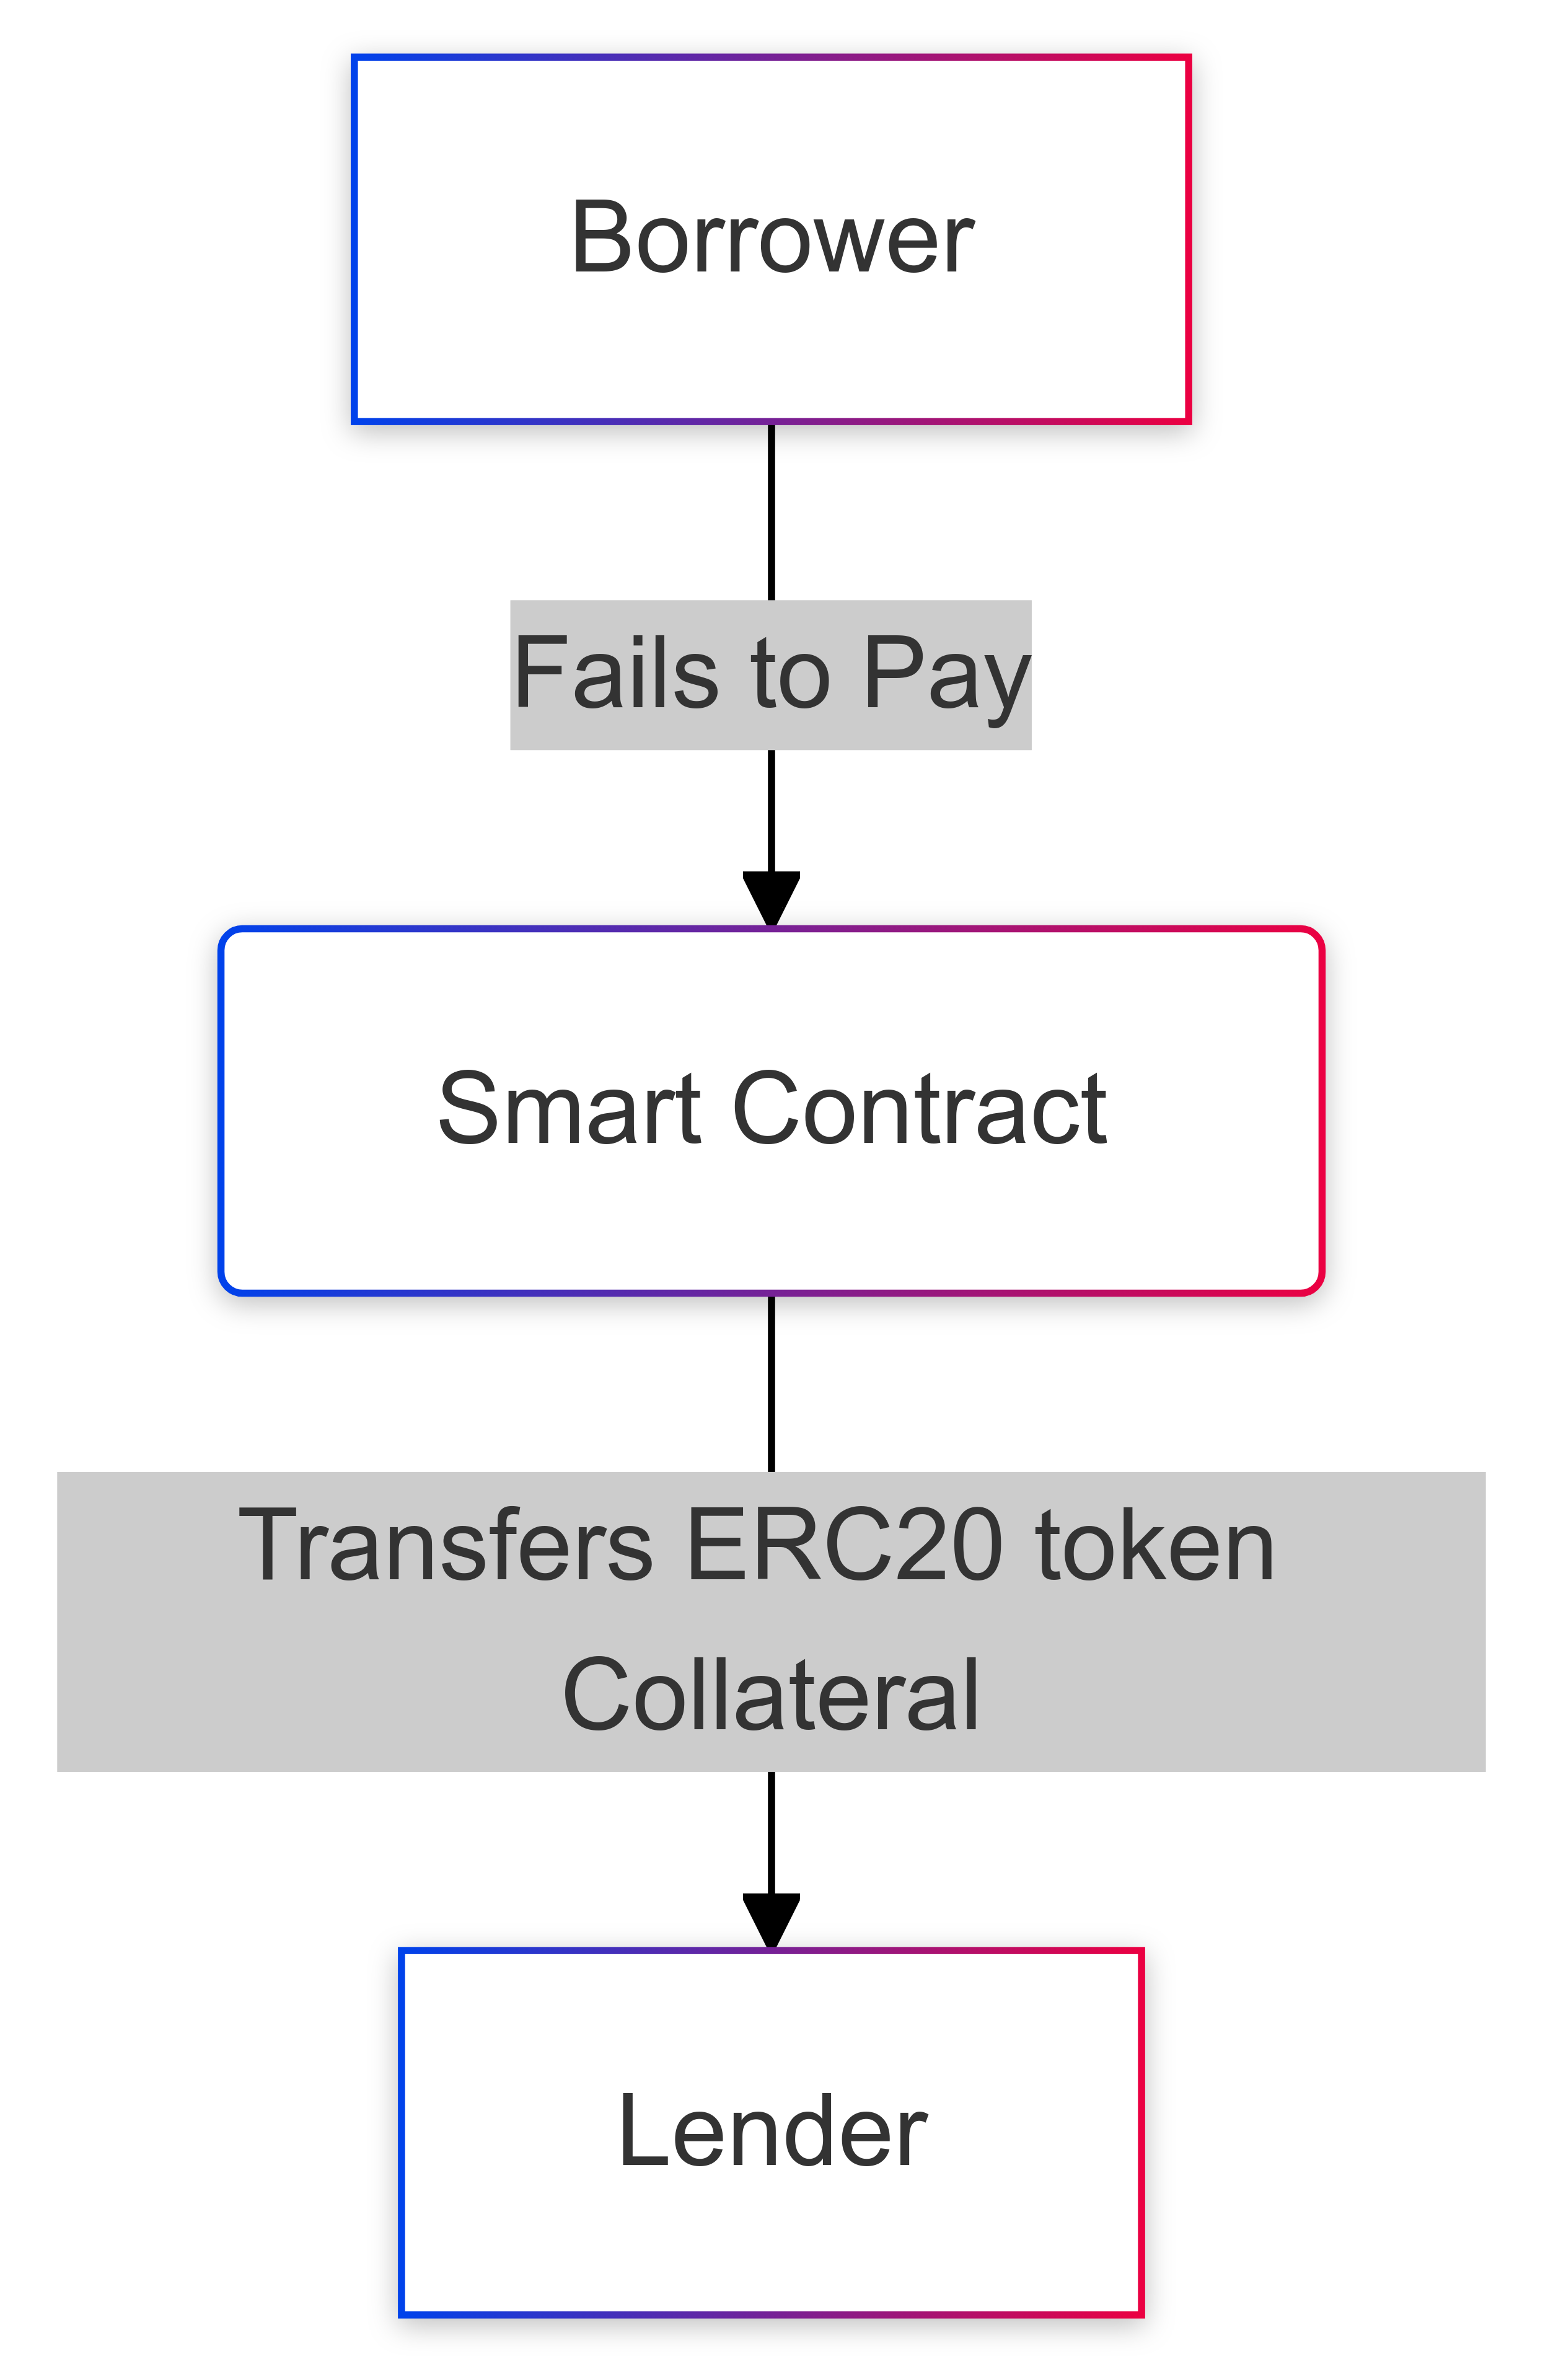
\includegraphics[width=\textwidth]{image/otcfailtopay}
        \caption{Borrower fails to repay the loan}
        \label{fig:fails}
    \end{minipage}
    \FloatBarrier
\end{figure}





Aave, from V1, breaks the P2P approach by creating lending pools where lenders deposit a cryptocurrency accepted by the protocol for the specific pool in exchange of a proxy token, receiving algorithmically calculated interest and borrowers borrow from the pool providing in exchange a collateral, chosen among the accepted ones from the protocol.
\begin{figure}[ht]
    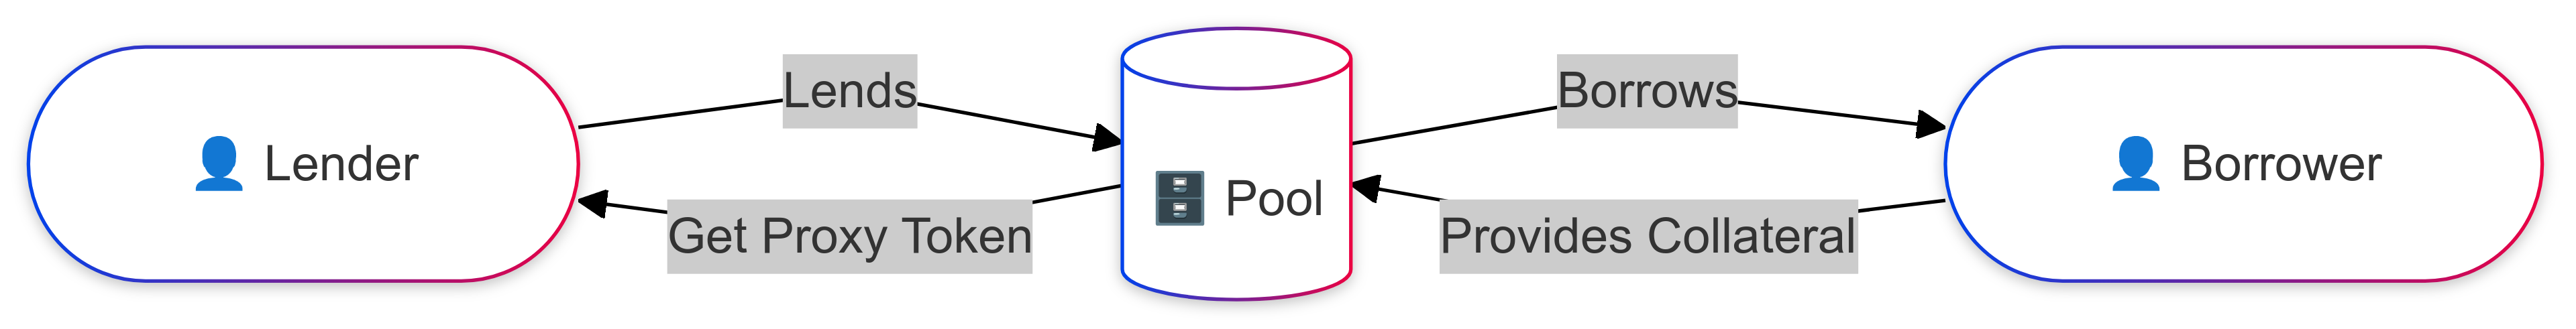
\includegraphics[width=0.7\textwidth]{image/lenderborrower.png}
    \caption{Aave standard lending borrowing}
\end{figure}
Borrowing can be at variable or fix rate and each borrowing position has an health factor ($H_f$) which potentially triggers, based on an algorithm, a liquidation for an under collateralised loan ($H_f$ below a calculated threshold). In traditional finance this can be similar to a margin call  with the addition of an upgradable protocol driving the calls based on mathematical functions proposed through a governance process.

\begin{table}[ht]
\centering
\caption{Comparison Between ethLend and Traditional Finance}
\begin{tabular}{ll}\toprule
\textbf{ethLend} & \textbf{Traditional Finance} \\ \midrule
Decentralized     & Centralized                \\
Peer-to-peer (P2P) & Over-the-counter (OTC)     \\
Fail to pay: Liquidation & Fail to pay: Liquidation \\ \bottomrule
\end{tabular}\\
%%\text{\footnotesize{Comparison between Aave V1 and traditional finance}}
\label{tab:ethlend_vs_trad_fin}
\end{table}

Aave V2 enhance V1 as gives the possibility of upgrading the proxy tokens given to lenders, reduces gas inefficiencies and simplifies code and architecture.
V1 has the merit of flashloans introduction and V2 allows to use them for collateral trading, which means swapping collateral without closing and reopening a position, loan repayments, margin trading, debt swaps and margin deposits. In table  \ref{tab:ethlend_vs_trad_fin} and table
 \ref{tab:aave_v2_vs_trad_fin} traditional finance is compared to ethlend and Aave V2 showing how well known processes have been translated in DEFI. 

\begin{table}[ht]
\centering
\caption{Comparison Between Aave V2 and Traditional Finance}
\begin{tabular}{ll}\toprule
\textbf{Aave V2} & \textbf{Traditional Finance} \\ \midrule
Decentralized & Centralized \\
Lending pool & (Derivative) market \\
Decentralized assessment of collateral & Collateral rating \\
Health Factor ($H_f$) & Margin definition \\
Collateral adjustments to avoid liquidation & Collateral adjustments to avoid liquidation \\
$H_f$ close to 1: Alarm & Collateral $< $Margin: Margin call \\
Collateral increase or liquidation & Collateral increase or liquidation \\ \bottomrule
\end{tabular}\\
\text{\footnotesize{This table compares Aave V2 and traditional finance approaches in lending and collateral management.}}
\label{tab:aave_v2_vs_trad_fin}
\end{table}


\subsection{Aave Lending pool contract}

\begin{figure}[ht]
    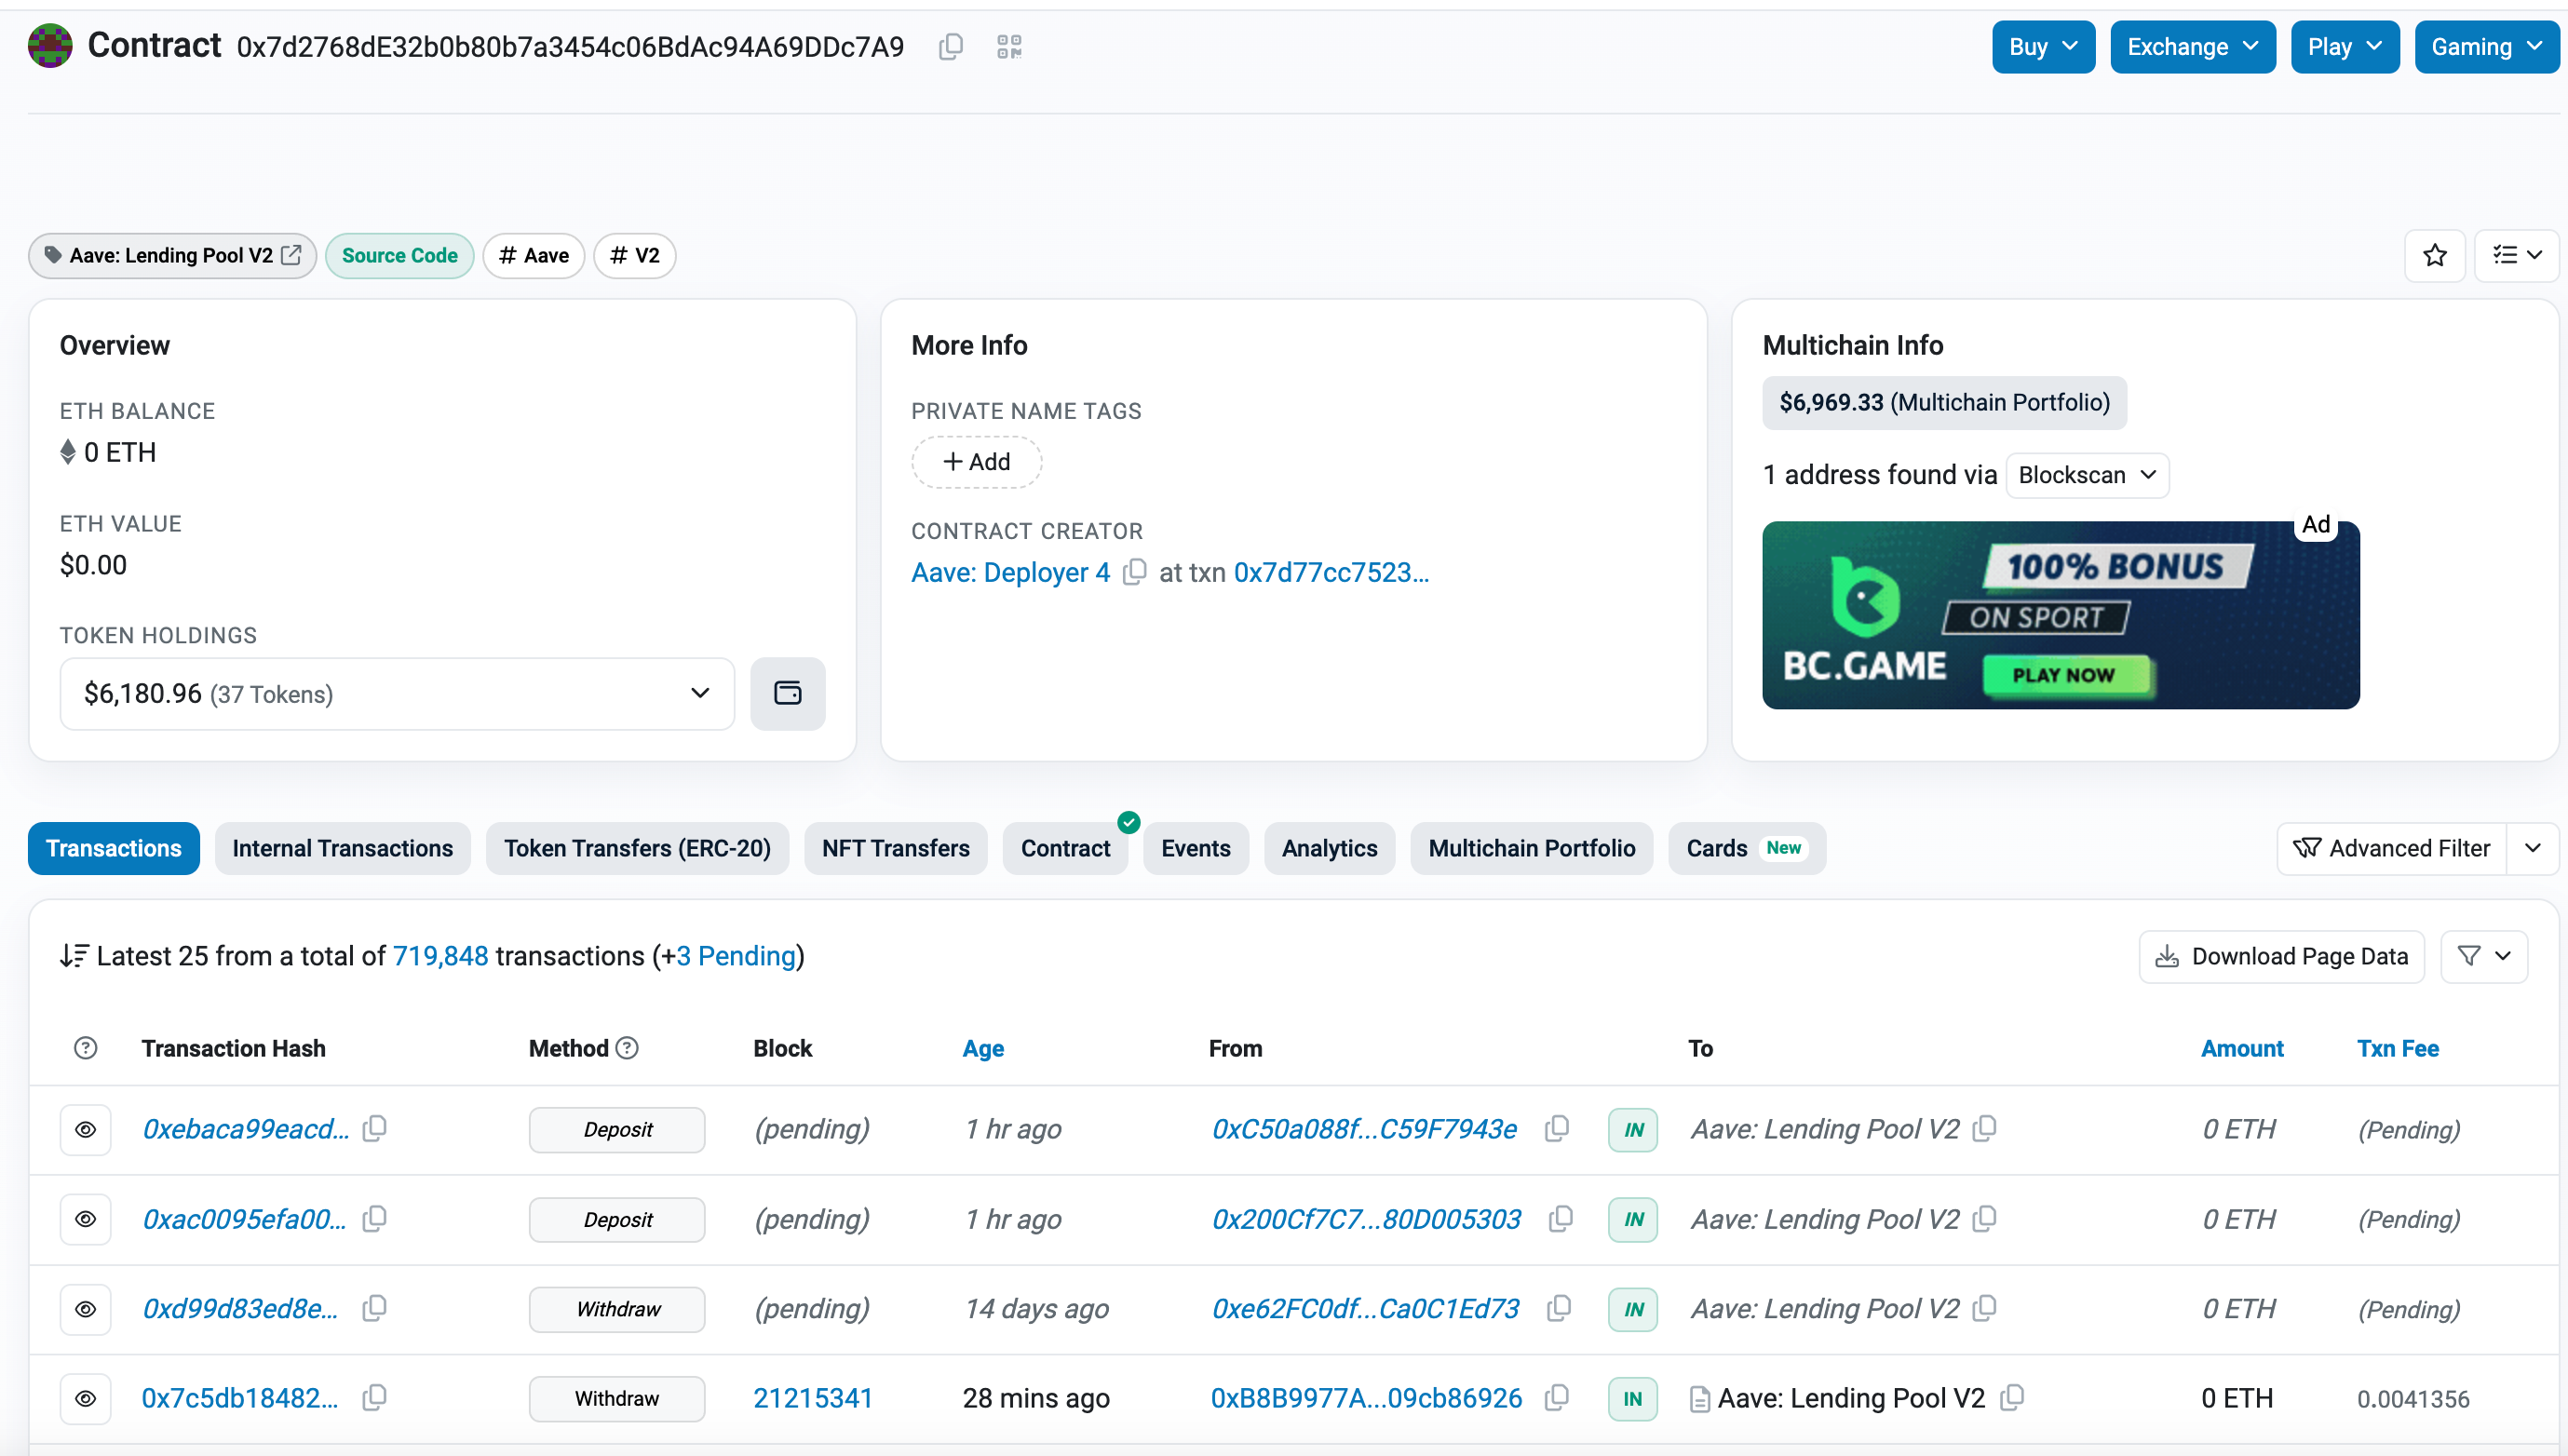
\includegraphics[width=1\textwidth]{image/etherscanLPool.png}
    \caption{Monitoring in etherscan Aave Lending Pool contract}
    \label{fig:etherscanLPool}
\end{figure}


A protocol based on ehtereum consists in a set of smart contracts. For the purpouse of Aave V2 flashloans a smart contract is handling the lending pool (including flashloan) calls. Such smart contract  is deployed on ethereum  as LendingPool  with contract address in ethereum main network: 0x7d2768dE32b0b80b7a3454c06BdAc94A69DDc7A9 which  includes calls which allow to deposit, redeem, borrow, repay, swap rate, liquidate, calling flash loans among others. This allows whoever has access to the ethereum blockchain to track the contract and the related transactions.

This paper  focus is on calls to LendingPool flashloan from ethereum inception to block number 20399999 correspondent to the date 27 July 2024.

\begin{table}[ht]
\centering
\caption{LendingPool Aave V2 Contract Methods}
\resizebox{\textwidth}{!}{%
\begin{tabular}{lll}\toprule
\textbf{Method Name} & \textbf{Synthetic Description} & \textbf{Keccak Selector} \\ \midrule
\texttt{deposit}     & Supply assets to the LendingPool to earn interest. & \texttt{0xe8eda9df} \\
\texttt{withdraw}    & Withdraw deposited assets from the pool.           & \texttt{0x6b91c3e7} \\
\texttt{borrow}      & Borrow assets from the pool against provided collateral. & \texttt{0x210dccae} \\
\texttt{repay}       & Repay a borrowed asset to restore collateral usage. & \texttt{0xb7ea3af4} \\
\texttt{swapBorrowRateMode} & Switch between stable and variable interest rates. & \texttt{0x95db9357} \\
\texttt{liquidationCall} & Liquidate undercollateralized positions in the pool. & \texttt{0x3bde6c10} \\
\texttt{flashLoan}   & Execute a flash loan with zero collateral requirements. & \texttt{0xee2e0890} \\ \bottomrule
\end{tabular}%
}
\caption*{\footnotesize This table summarizes key methods of the Aave V2 LendingPool contract, including their Keccak-encoded selectors.}
\label{tab:lendingpool_methods}
\end{table}

The table above includes keccak Selector info. This is the way the contract and method calls  are persisted on the blockchain.

\subsection {Flashloans}

When a loan is issued a lending protocol as well as in traditional finance is expecting a collateral or a cashflow as a guarantee. \uline{Flashloans are unique in the blockchain environment as they don't require neither a collateral nor a cash flow, provided that the loan is paid, interests included, within the same ethereum transaction. If the loan is not repaid the transaction is rolled back, at the cost for the borrower of the gas needed for processing the aborted transaction}. 
\begin{figure}[ht]
    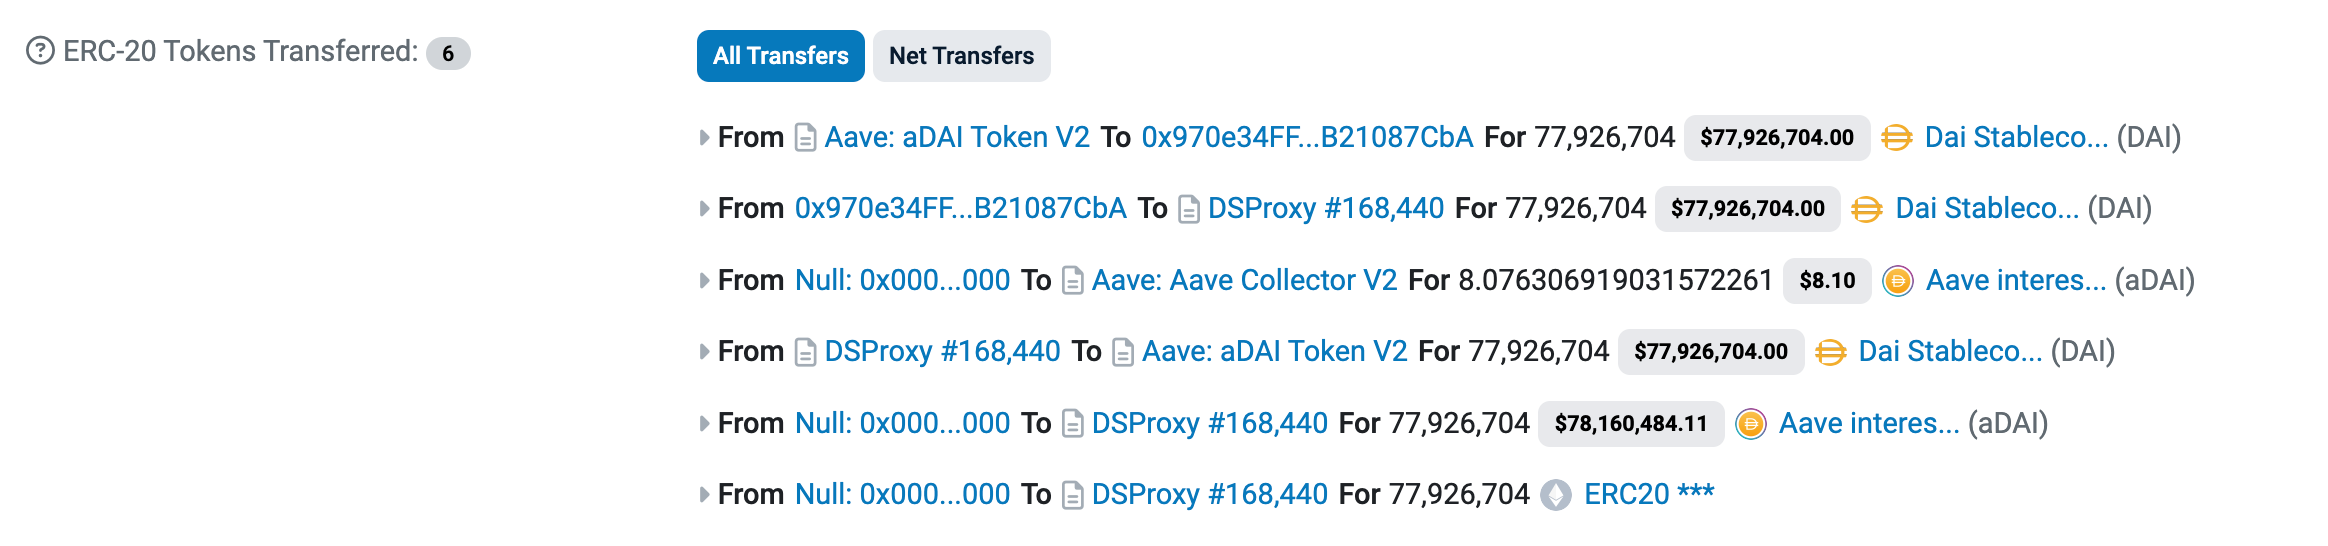
\includegraphics[width=1\textwidth]{image/flashloan.png}
    \caption{Example of a  flashloan}
    \label{fig:etherscanFLoan}
\end{figure}

The figure \ref{fig:etherscanFLoan} shows the transactions wrapped in a flashloan one. It is possible to recognize the opening of the loan, \ref{fig:etherscanreqFLoan}and the repayment with interests,  \ref{fig:etherscanrepFLoan}.

\begin{figure}[H]
    
\includegraphics[width=1\textwidth]{image/requestFlashloan.png}
    \caption{Request of the  flashloan}
    \label{fig:etherscanreqFLoan}
\end{figure}

\begin{figure}[H]
    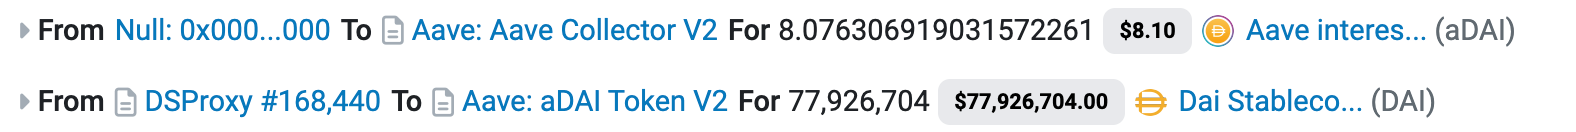
\includegraphics[width=1\textwidth]{image/repayFlashloan.png}
    \caption{Repayment of the  flashloan with interest}
    \label{fig:etherscanrepFLoan}
\end{figure}


Flashloans are the main topic of this paper therefore is critical to clarify how they work. It is extremely common when reading documentation or articles to get confused by the statement that the repayment should happen within the same ethereum transaction: this can be misleading as with ethereum transaction, in this case is intended a transaction which can hold even hundreds of inner transactions as it is showed in Figure \ref{fig:etherscanFLoan}. This example shows a flashloan constituted of just six transactions as it has been chosen quite simple for the specific purpose.
It is common at this point to be confronted with the question how can many transactions be performed and, in some cases, rolled back.
To clarify this  it is crucial to recall the definition of transactions and block. Transactions are intended to be cryptographically signed instructions sent from one Ethereum account to another where the account can be a public address associated to private keys typically controlled by a person or a contract account associated to a smart contract and controlled by code, whereas a  block  is a component of the chain, containing among the others a set of transactions and the information to rebuild the chain itself. The nature of blockchain permits the creation of flashloans cause if a set of operations, in this case inner transaction within the flashloan one, is not ending with the full repayment, all the operations will be aborted by not being added to the block, therefore not ending in the blockchain. The flashloan is therefore computed in a precommit phase and the persistency in the blockchain is subordinated to the repayment plus interests.. The described behaviour leads to the creation of an instrument which doesn't exists in traditional finance and is comparable to a rollback in a traditional relational database where the atomic operation corresponds the set of inner transaction wrapped by the flash loan one. 

\begin{table}[ht]
\centering
\caption{Comparison Between Flashloans and Databases}
\resizebox{\textwidth}{!}{%
\begin{tabular}{ll}\toprule
\textbf{Flashloans} & \textbf{Databases} \\ \midrule
Decentralized & Centralized \\
Open flashloan, inner transactions, repay flashloans & Begin transaction, internal transactions, end transaction \\
Add or not to the block & Commit or rollback \\
Block added to the chain & Persist operation in DB \\ \bottomrule
\end{tabular}%
}
\caption*{\footnotesize Flashloans have no counterpart in traditional finance. The best fit for a comparison is a transactional process in traditional databases.}
\label{tab:flashloans_vs_db}
\end{table}



Flashloans  are not enabling the user to get an infinite loan: borrowing enabled and the liquidity of the pool, as a bigger amount than the pool size  itself cannot be accessed, are the constraints.


\newpage

\section{Self hosted Ethereum node}
\subsection {Introduction}
Ethereum is a distributed network of computers (known as nodes) running software that can verify blocks and transaction data. This is achieved by running on each computer of the network a client software which fullfills the ethereum specification. There are many implementation of such software and, provided that they fullfill all the protocol requirement, the nodes can interact independently from the  implementation they run. 
\begin{figure}[ht]
    \scalebox{1.4}{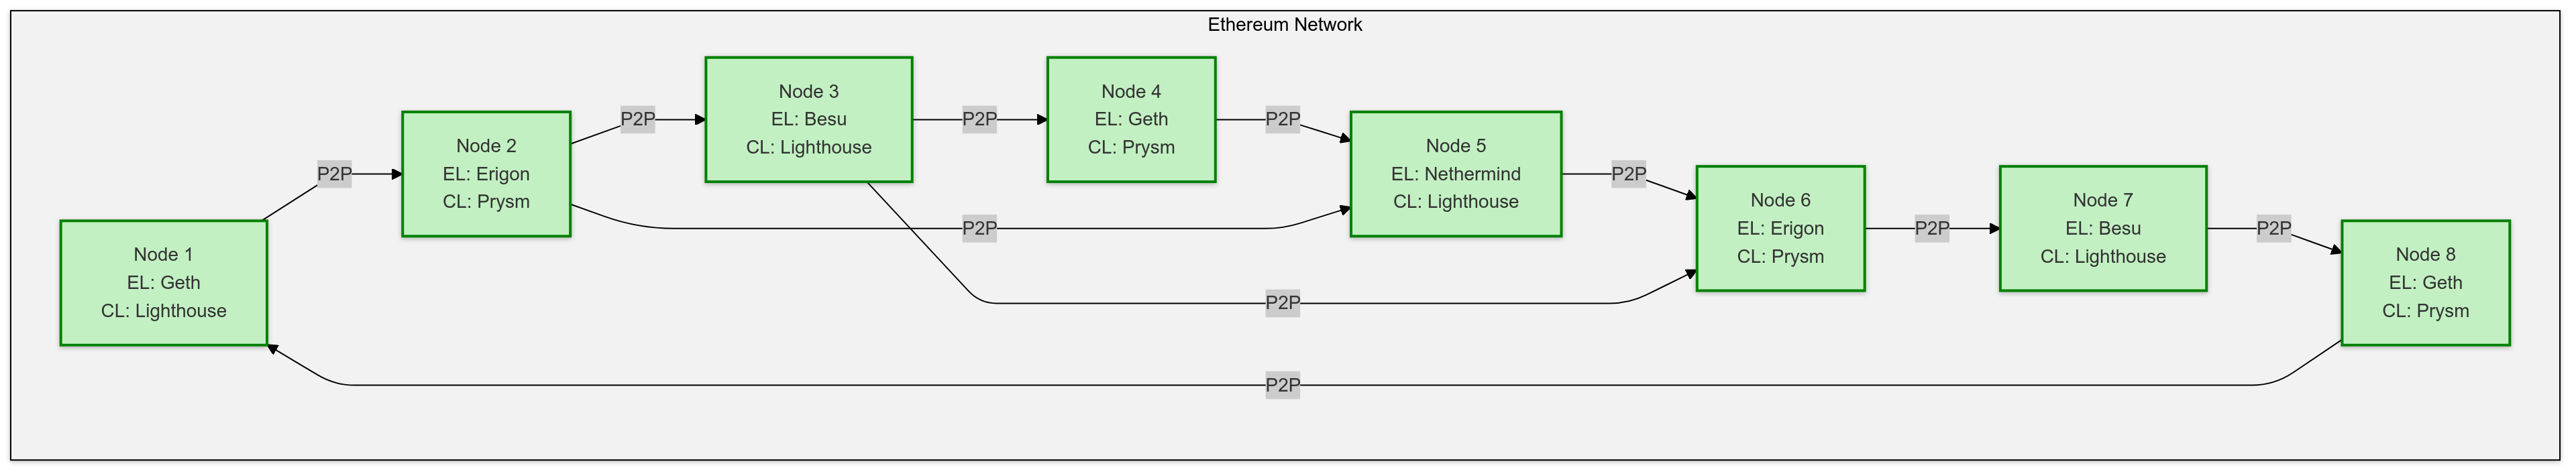
\includegraphics[width=0.7\textwidth]{image/simpleethnodes.png}}
    \caption{Simplified view of ethereum nodes}
    \label{fig:ethnodes}
\end{figure}

The figure \ref{fig:ethnodes} represents few nodes interacting. A node is any instance of Ethereum client software that is connected to other computers also running an Ethereum client software, forming a network. A client is an implementation of Ethereum that verifies data against the protocol rules and keeps the network secure. The figure \ref{fig:ethnodes} represents the current ethereum  state with a transition  from proof of work to proof of stake where a node has to run two clients, a consensus client and an execution client,  which come with different possible implementations. The execution client, also known as the Execution Engine, EL client or formerly the Eth1 client, listens to new transactions broadcasted in the network, executes them in EVM (Ethereum Virtual Machine), and holds the latest state and database of all current Ethereum data. The consensus client, also known as the Beacon Node, CL client or formerly the Eth2 client, implements the proof-of-stake consensus algorithm, which enables the network to achieve agreement based on validated data from the execution client. All these clients work together to keep track of the head of the Ethereum chain and allow users to interact with the Ethereum network. 

\subsection {Self hosted node vs provider}
This paper is written processing data from a self hosted node. That is not mandatory as it is possible to rely on services created ad hoc. Infura and Alchemy are popular third-party services that provide easy access to Ethereum nodes via APIs, allowing developers to interact with the Ethereum blockchain without running their own node. These services abstract the complexities of node management and provide scalable infrastructure for dApps, smart contract deployments, and blockchain analytics.
Using such services has the advantage of providing a standardised environment out of the box but comes with some disadvantages. On a bulk analysis API calls can get expensive, there is not a full control on the data accessed, the providers can block access and there are centralisation risks which are exacerbated by relying fully on third party providers.
Additionally external providers implies  a lack of control on data while a node implementation gives both the control and tools for accessing such data: being this paper based on data analysis, the choice of a local node provider suitable to self hosting has been prioritised.
Running a node is not  trivial at the current stage of the ethereum network. An archive node can require more than 10 TB disk space with certain implementations, a good bandwidth, fast disks and a computer with 32 Gb Ram and multicore.
The next sections address the choice of node type and client implementation

\begin{table}[ht]
\centering
\caption{Main characteristic Alchemy and Infura}
\resizebox{\textwidth}{!}{%
\begin{tabular}{ll}\toprule
\textbf{Alchemy} & \textbf{Infura} \\ \midrule
Advanced developer tools (e.g., debug API, enhanced APIs) & Basic Ethereum and IPFS API services \\
Performance optimizations (e.g., caching, load balancing) & Standard JSON-RPC API services \\
Customizable notifications and alerts & Basic webhook notifications \\
Higher-tier analytics for transaction debugging & Minimal analytics support \\
Enterprise-grade SLAs with premium support & Standard-tier SLAs \\ \bottomrule
\end{tabular}}
\label{tab:alchemy_vs_infura}
\end{table}

\begin{table}[ht]
\centering
\caption{Main characteristic Infura, Alchemy, and Self-Hosting a Node}
\resizebox{\textwidth}{!}{%
\begin{tabular}{p{0.3\textwidth} p{0.3\textwidth} p{0.3\textwidth}} \toprule
\textbf{Infura} & \textbf{Alchemy} & \textbf{Self-Hosting a Node} \\ \midrule
Cloud-hosted Ethereum and IPFS APIs & Enhanced APIs for analytics and debugging & Requires physical or virtual machine setup \\ \midrule
No need for hardware or sync maintenance & Managed infrastructure with performance optimizations & Full control over node and data \\ \midrule
Limited archive node access on basic plans & Advanced caching and query optimization & Can configure full or archive nodes as needed \\ \midrule
Third-party dependency & Dependency on Alchemy services & Full decentralization and sovereignty \\ \midrule
Quick and easy setup for development & Cloud-hosted, easy to scale & Longer setup time, requires technical expertise \\ \midrule
Usage limited by rate limits and quotas & Developer-focused tools (e.g., Notify API, transaction explorer) & Unlimited usage, depends on hardware capacity \\ \bottomrule
\end{tabular}}
\label{tab:infura_alchemy_self_hosting}
\end{table}


\subsection {Comparison of full nodes vs archive nodes in various ethereum implementations}

Ethereum nodes come in different types based on the amount of data they store and the roles they serve in the network. Running a self hosted node to perform data analysis requires to choose between a full node and an archive node.

A full node stores the complete current state of the Ethereum blockchain (i.e., account balances, contract storage, etc.) and recent historical data, but it prunes old state data to save space. Full nodes verify all transactions and blocks from the genesis block to the current state but don't keep every historical state like past balances or contract storage at every block.
An Archive Node stores everything that a full node does, but in addition, it keeps all historical states for every block in the blockchain. This means archive nodes can provide the exact state of the blockchain at any point in history, but they require significantly more disk space. Full nodes are sufficient for most operations, while archive nodes are only necessary to access to the entire historical state of the blockchain.


A full node stores enough information to partecipate to the ethereum network, also as validator, but data analysis would become cumbersome as the stored information is enough to rebuild and validate the current state but requires computation to do it: for this paper the archive node is therefore the best choice. 


\subsection {Motivation for choosing Erigon}


\begin{table}[H] % Use [H] to enforce placement
\centering
\caption{Resource Requirements for Ethereum Clients}
\resizebox{\textwidth}{!}{%
\begin{tabular}{lccccc}\toprule
\textbf{Client} & \textbf{Full Node Disk} & \textbf{Archive Node Disk} & \textbf{Full Node RAM} & \textbf{Archive Node RAM} & \textbf{CPU Requirements} \\ \midrule
Erigon & 400--500 GB & $\sim$3.5 TB & 2--8 GB & 8--16 GB & Optimized (low-medium) \\
Geth & 800--900 GB & $\sim$10 TB & 4--16 GB & 16 GB or more & High (sync heavy) \\
Besu & 800--900 GB & $\sim$10 TB & 8--16 GB & 16--32 GB & Medium \\
Nethermind & 700--900 GB & 6--8 TB & 4--8 GB & 16 GB or more & Optimized (medium) \\
Lighthouse, Prysm & 10--30 GB (Beacon) & N/A & 1--4 GB (Beacon) & N/A & Low \\ \bottomrule
\end{tabular}%
}
\captionsetup{font=footnotesize, justification=centering}
\caption*{\footnotesize This table lists the resource requirements for different Ethereum clients, including disk and RAM usage, and CPU demands for full and archive nodes.}
\label{tab:ethnodes}
\end{table}

There are many implementations of archive nodes and the proper selection is related to  data analysis suitability: save disk space, fast access to data, a client which allow to present the data in an human readable format for easy interpretation. For this purpose  the most common implementations have been tested. The table  \ref{tab:ethnodes} summarises resource requirements for the most common node implementations. 
Geth is the most widely used Ethereum client, Erigon is designed to be more resource-efficient than traditional Geth, especially in terms of disk usage and sync time.
Besu is an Ethereum client written in Java, commonly used in enterprise environments.
Nethermind is a high-performance Ethereum client written in C\# with a focus on speed and configurability.
Besu and Geth may require more memory depending on the workload.

For the present purpose, a combination of Geth and Lighthouse was tested  (the latter only for consensus) as well as  Geth and Besu; the test of geth and besu aborted while the  second SSD disk installed as volume was half filled (max capacity 10 Tb and strong performance degradation).  Nevermind has not been tested as, being written in C\#, is strongly suboptimal to work on a linux instance: the data related to it are an estimation).
Considering the data presented in Table \ref{tab:ethnodes} Erigon looks the best fit, because it allows to run an archive node with a standard 4tb ssd disk. All ethereum node are very demanding in term of read write disk performance, therefore maximising the IO would be a plus, and two SSD in raid-0 are a good choice but not mandatory. 
\begin{figure}[ht]
    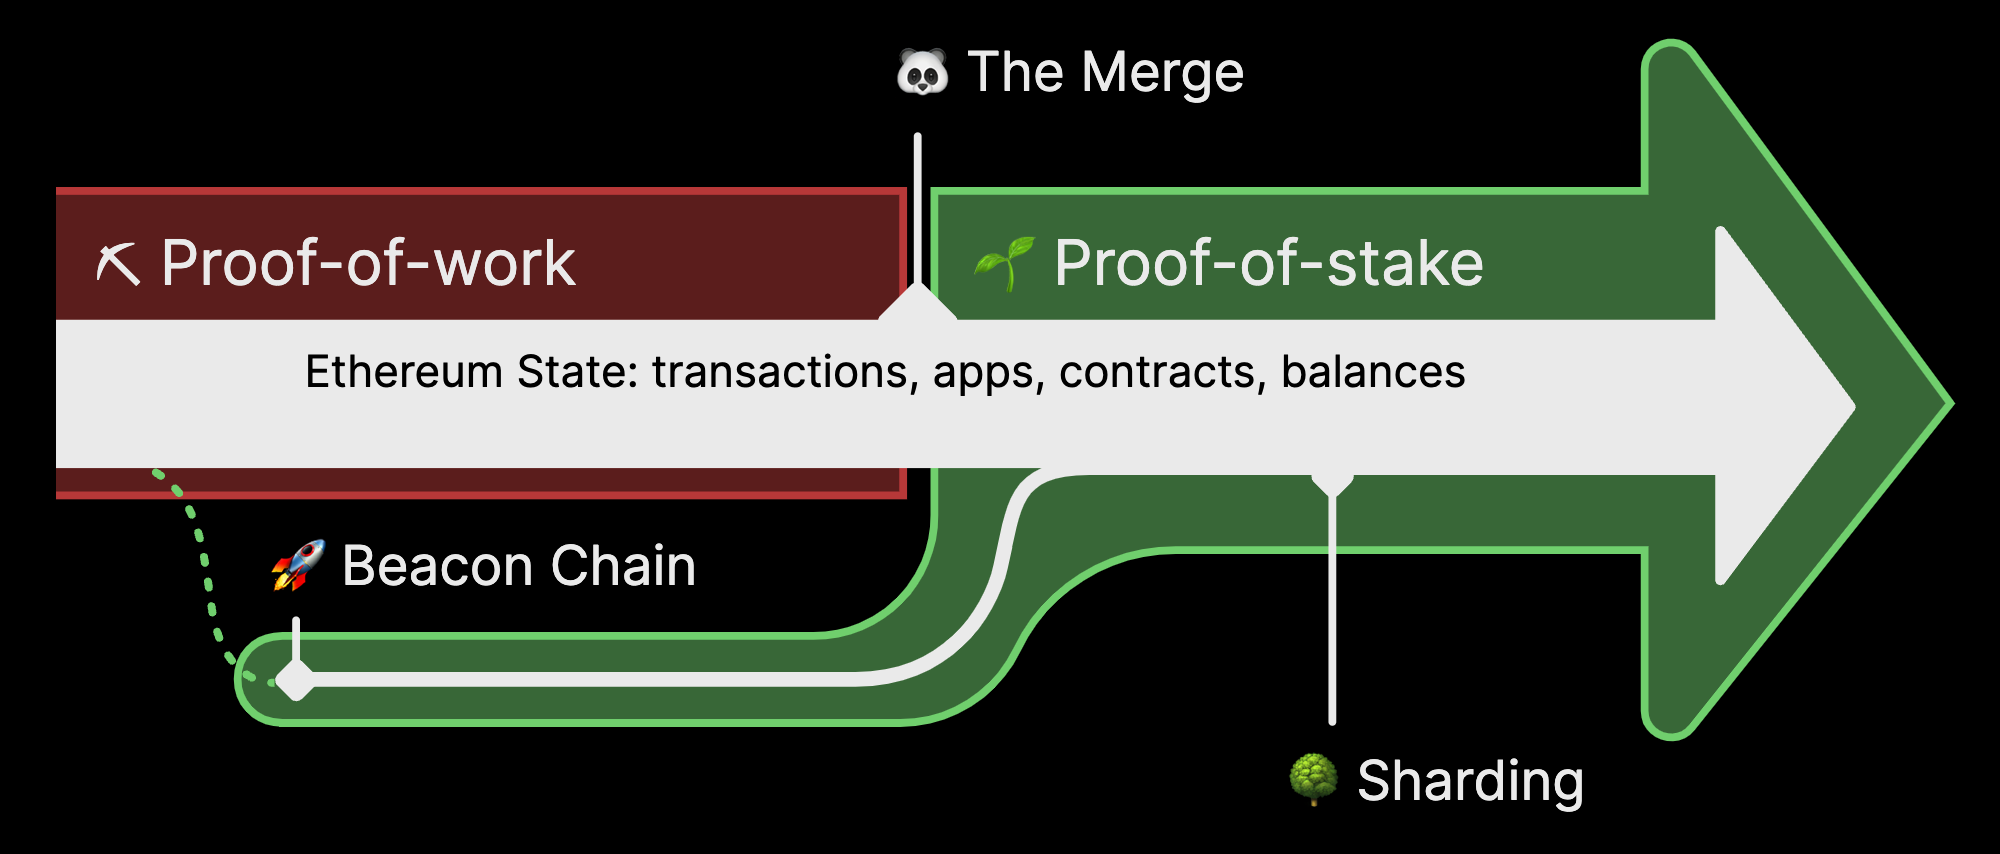
\includegraphics[width=0.7\textwidth]{image/powpos.png}
    \caption{Ethereum merge}
    \label{fig:powpos}
\end{figure}

Another advantage of Erigon is having an embedded consensus node implementation. Since the merge, which is represented in figure \ref{fig:powpos}, when ethereum became proof of stake, there is the need of an execution node and a consensus node. As showed in the picture for some time the consensus and execution layers run in parallel and they were consolidated in a unique chain with the merge; the consequence  for data analysis is that  the simplest is the consensus the best as the meaningful data are held in the execution layer. This is the case of caplin, the embedded consensus node in erigon, as it allows to achieve an archive node full synch without any configuration or installation of a compatible consensus node.
Before starting the work in the main chain  Erigon was tested on sepolia, a light test network, and verified that the data saved in a key value db, mdbx, were properly indexed and rendered by the embedded UI, otterscan. The last requirement for the analysis is being able to stop the synch at a certain block and run an rpc (remote procedure call) server which serves the data without synching continuously. Erigon satisfy also this. This allows to synch just once the main network till the desired block and then stop this operation, extremely resource demanding in term of bandwidth even when close to the ethereum chain tip.
An additional section addresses otterscan compared to other ethereum UI like etherscan and blockscout.
The table \ref{tab:adverigon} summarises erigon advantage for self hosted data analysis:


\begin{table}[ht]
\centering
\caption{Erigon Advantages for Data Analysis}
\begin{tabular}{cccc} \hline\hline
\textbf{Advantage} \\ \midrule
Embedded consensus \\
Low disk usage \\
Fast read \\
UI integrated \\
Geth tools available out of the box \\ \bottomrule
\end{tabular}\\
\text{\footnotesize{This table lists the key advantages of using Erigon for data analysis.}}
\label{tab:adverigon}
\end{table}

\newpage


\section{Blockchain explorers}
\subsection{Introduction} 
\label{bexp:lintro} 
Blockchain data are saved linearly in time in blocks keeping a reference to the predecessor, giving origin to a storage structure which is optimised for a decentralised environment but not for data analysis.  A comparison among  well known data storage techniques like  relational databases, key value databases and  nosql ones gives an idea of how storing data answers to different problematics.\\
A traditional relational database (oracle) is a tool thought to store data in a centralised way with a focus on data atomicity, consistency, isolation and durability (ACID). This characteristics together with scalability and a language, sql, strictly declarative and then optimisable in execution from the db engine itself, are the main reasons of the large success of relational db in the corporate environment. \\
Another way of storing data is represented by nosql dbs which come as Key-value pair,Document-oriented, Column-oriented and Graph-based.
Key value databases have recently found plenty of application: mimicking an hasthable (map) data structure, they are  providing an extremely fast  read access and are scalable in a cloud architecture. Such a data structure found the first application in caches, generalising at a cloud level, what was already known in the host environment with tools like memcache and other similar ones as cask. In a cloud environment and, in general, in a network intensive environment, key value db like level2 and mdbx have found great applications and they are the core of many ethereum client software like geth and erigon where storage size and faast read access are important. \\
Another storage, very common nowadays is the so called  graph db whose implementation examples are neo4J or mongoDb. A  relevant application of such dbs is storing hierarchical data in a natural way, which is prevented by  design in a relational db: graph data structures, payload of web services, xml and json data format as the web page structure itself are all best suited to be handled through graph db. \\
Document and column database have found a great traction in the cloud environment related to big data: while a relational db is optimal in corporate to store data 'polished' and consistent, a document or columnar db allows to quickly store giant amount of unstructured data which can be processed and structured in later steps. A typical scenario is to have applications which are processing the nosql data to polish them and store the extracted and transformed data subset in a relational DB.






It is clear, from table \ref{tab:dbtypes}  that each data storage has a clear motivation and, apart from legacy systems, where they can be misused because of the difficulty of migrating data while keeping business requirement, in greenfield projects it is natural to chose the most convenient data storage based on requirements.
In a blockchain the data persistency for  analysis is a secondary requirement and a set of tool have been created to facilitate this task. The main categories are two: ETL (extract transform load) systems, where data from the ethereum client are accessed in read mode, transformed and loaded (persisted) in a 3rd party DB which is selected for pure data analysis  or direct access to indexed data of the ethereum client.There are four main types of interactions with the ethereum client: direct query of blockchain data, a programmatic approach on the node itself, UI rendering of indexed data of the node, query of data stored in third party DBs via sql or programmatically, UI rendering of data in third party DB. 


\begin{table}[ht]
\centering
\caption{Database Types, Implementations, and Usage}
\resizebox{\textwidth}{!}{%
\begin{tabular}{p{0.3\textwidth} p{0.3\textwidth} p{0.4\textwidth}} \toprule
\textbf{Database Type} & \textbf{Implementations} & \textbf{Usage} \\ \midrule
Relational & MySQL, PostgreSQL, Oracle & Structured data management, Transactions \\ 
Key-Value & LevelDB, MDBX , AWS DynamoDB & Fast read access,  Low footprint \\ 
Graph DB & Neo4j,  MongoDB & Hierarchical, Connected structures \\ 
Document DB & MongoDB & Big data, Data lakes \\ 
Columnar DB & Google BigQuery & Big data, Analytics \\  \bottomrule
\end{tabular}%
}
\label{tab:dbtypes}
\end{table}



For the purpose of this work it is strongly advantageous to have an application which allows to visualise the transactions stored in the node. This is normally achieved through UI web applications, where the browser is the natural UI client, called blockchain explorers. These UI could access data indexed in the node or moved through ETL to 3rd party db. In the next sections is presented and motivated the choice for the explorer lately used in flashloans analysis.



\subsection{Blockchain explorer usage}

A blockchain explorer is a webapp UI which plays the role of crucial tool for viewing, analyzing, and understanding data on a blockchain. It transforms complex, encoded information into human-readable form, making it easier to track transactions, verify addresses, explore smart contracts and can perform, in some case, some statistical analysis on behalf of the end user. Without a blockchain explorer, transaction data and smart contract interactions appear as hex-encoded information, which is not human-readable: below a set of pictures of a transaction in etherscan (the most used blockchain explorer), in otterscan (the explorer integrated in erigon) and raw data polling the node shows the difference between raw data and the same data rendered in an explorer making evident the importance of using properly an explorer or a combination of them.


\begin{figure}[ht]
    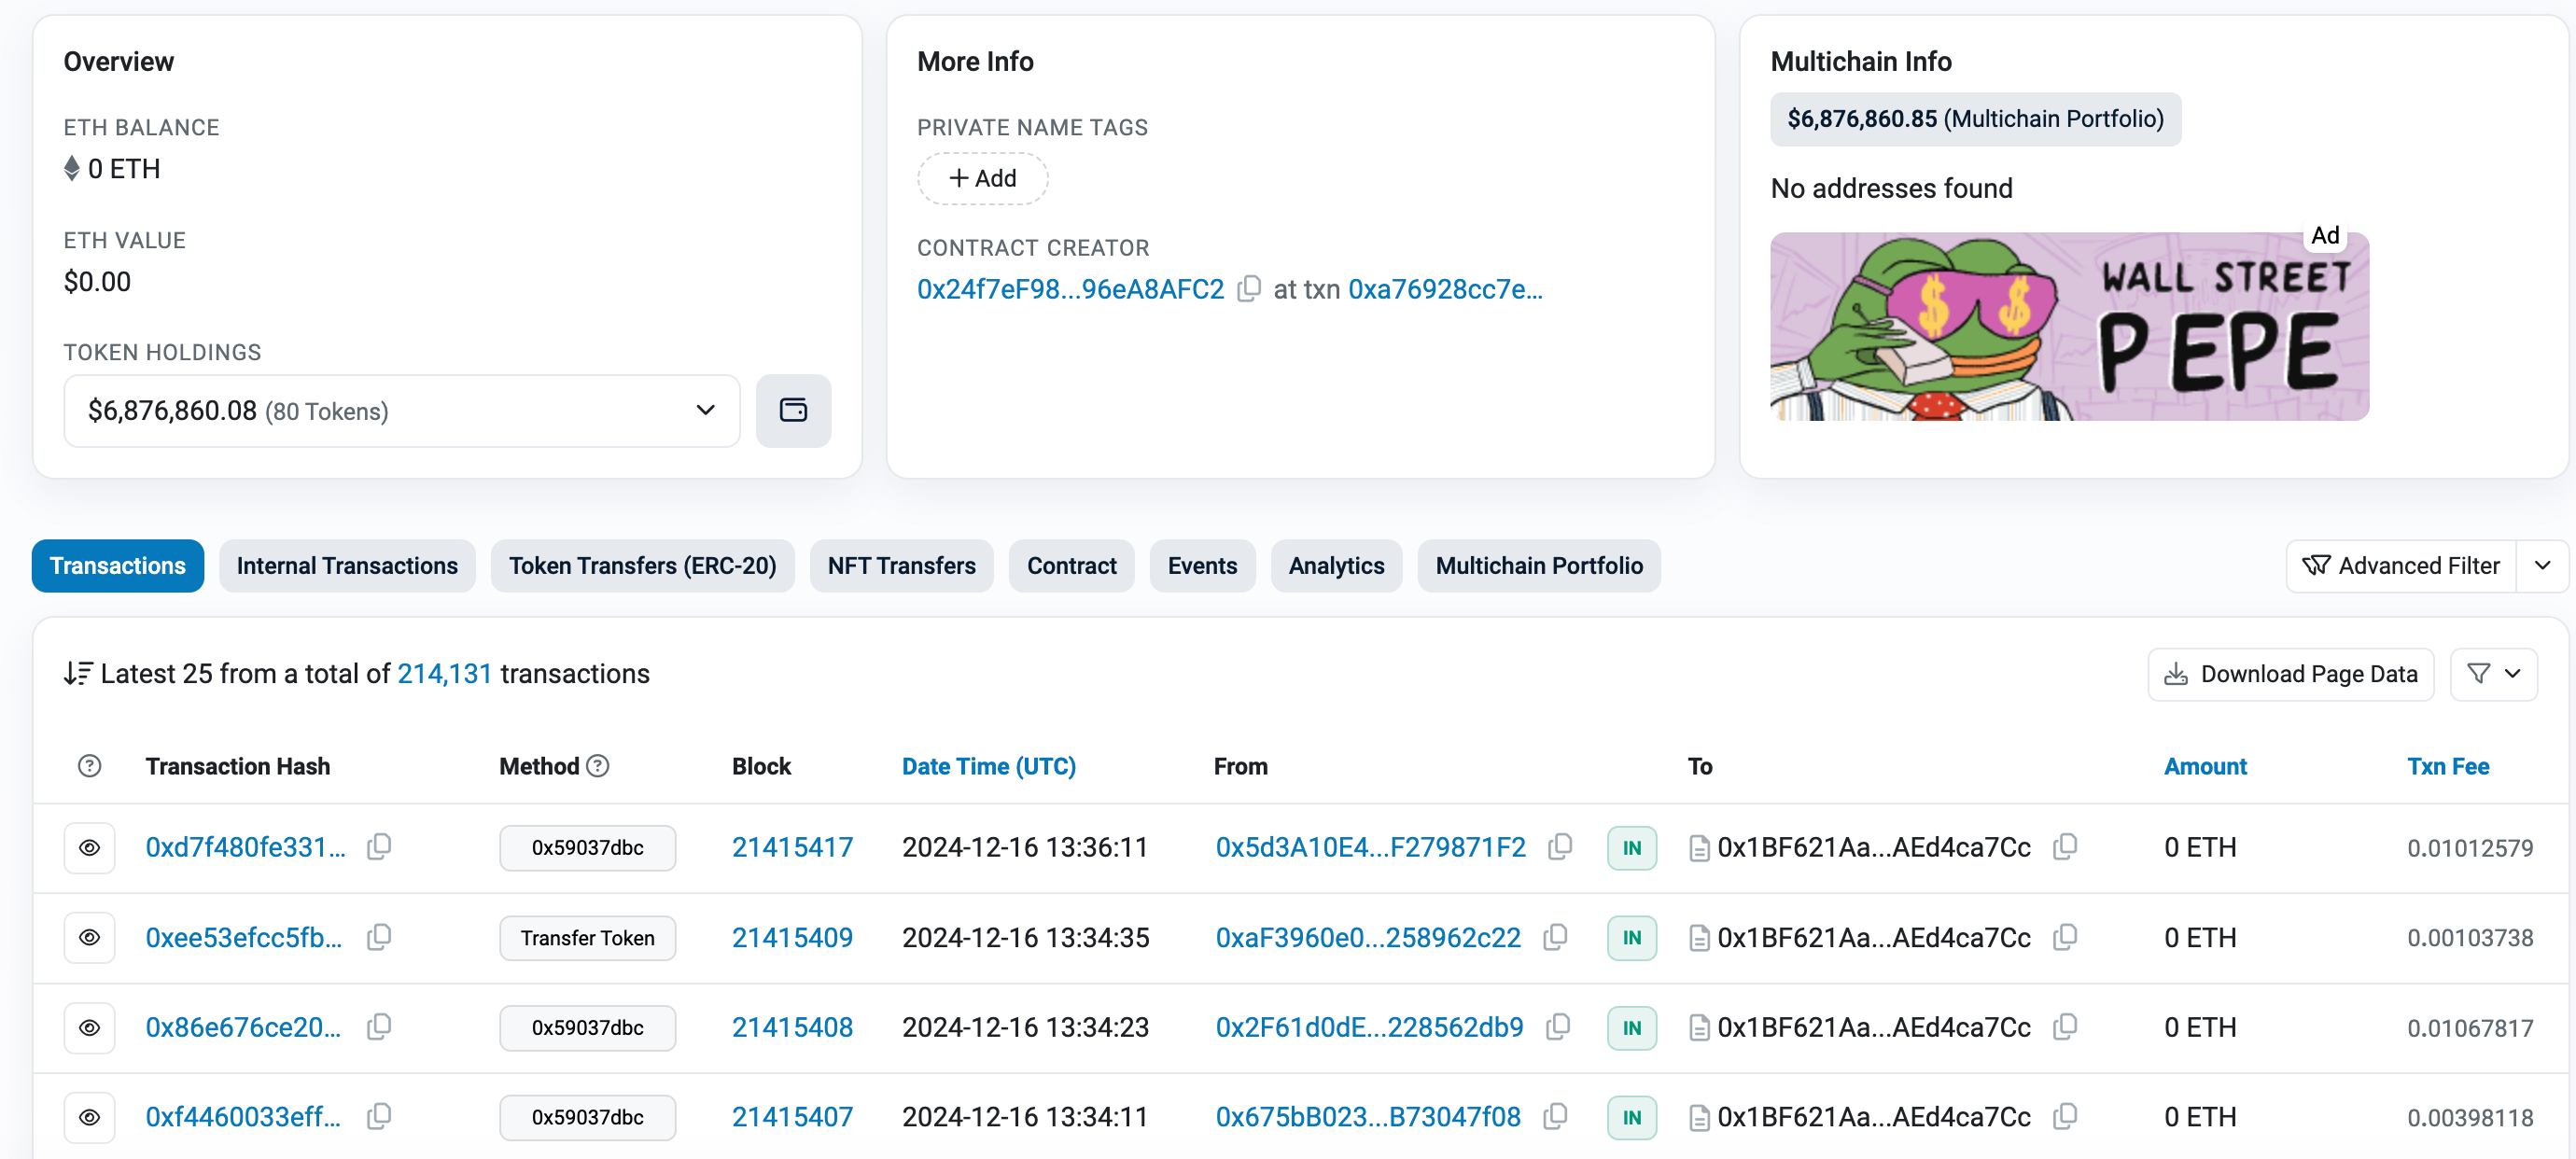
\includegraphics[width=1.0\textwidth]{image/explorers/uniswapLPetherscan.png}
    \caption{View LP USDC-WETH in etherscan}
    \label{fig:ethlp}
\end{figure}

The figure \ref{fig:ethlp} shows a liquidity pool in Uniswap V3 through etherscan.  Uniswap is the most famous and widely used decentralized exchange, therefore a primary Defi primitive (the term primitive is part of Defi lingo and indicates a building block of potentially larger processes where many primitives are connected),  which allows to swap tokens through decentralised trading pairs. The protocol is quite complex and this paper doesn't aim to explain how it works, but  it represent  a good example of how a blockchain explorer can simplify the analysis of a transaction. The liquidity pool that is represented in the picture is created triggering another smart contract (uniswap liquidity pool factory) and there are plenty of similar  pools of trading pairs created the same way. The specific pool  is the trading pair USDC-WETH, two ERC-20 tokens (ERC-20 is a standard for tokens on the ethereum blockchain, that defines a set of features and rules for issuing and managing tokens ensuring interoperability ) who have a considerable liquidity. 


\subsection{Analyse transactions in blockchain explorers}

Given a contract view like in figure \ref{fig:ethlp}, it is possible to expand one of the  transactions triggered by it: in the figure below is showed a swap (exchanging a token for another).




\begin{figure}[ht]
    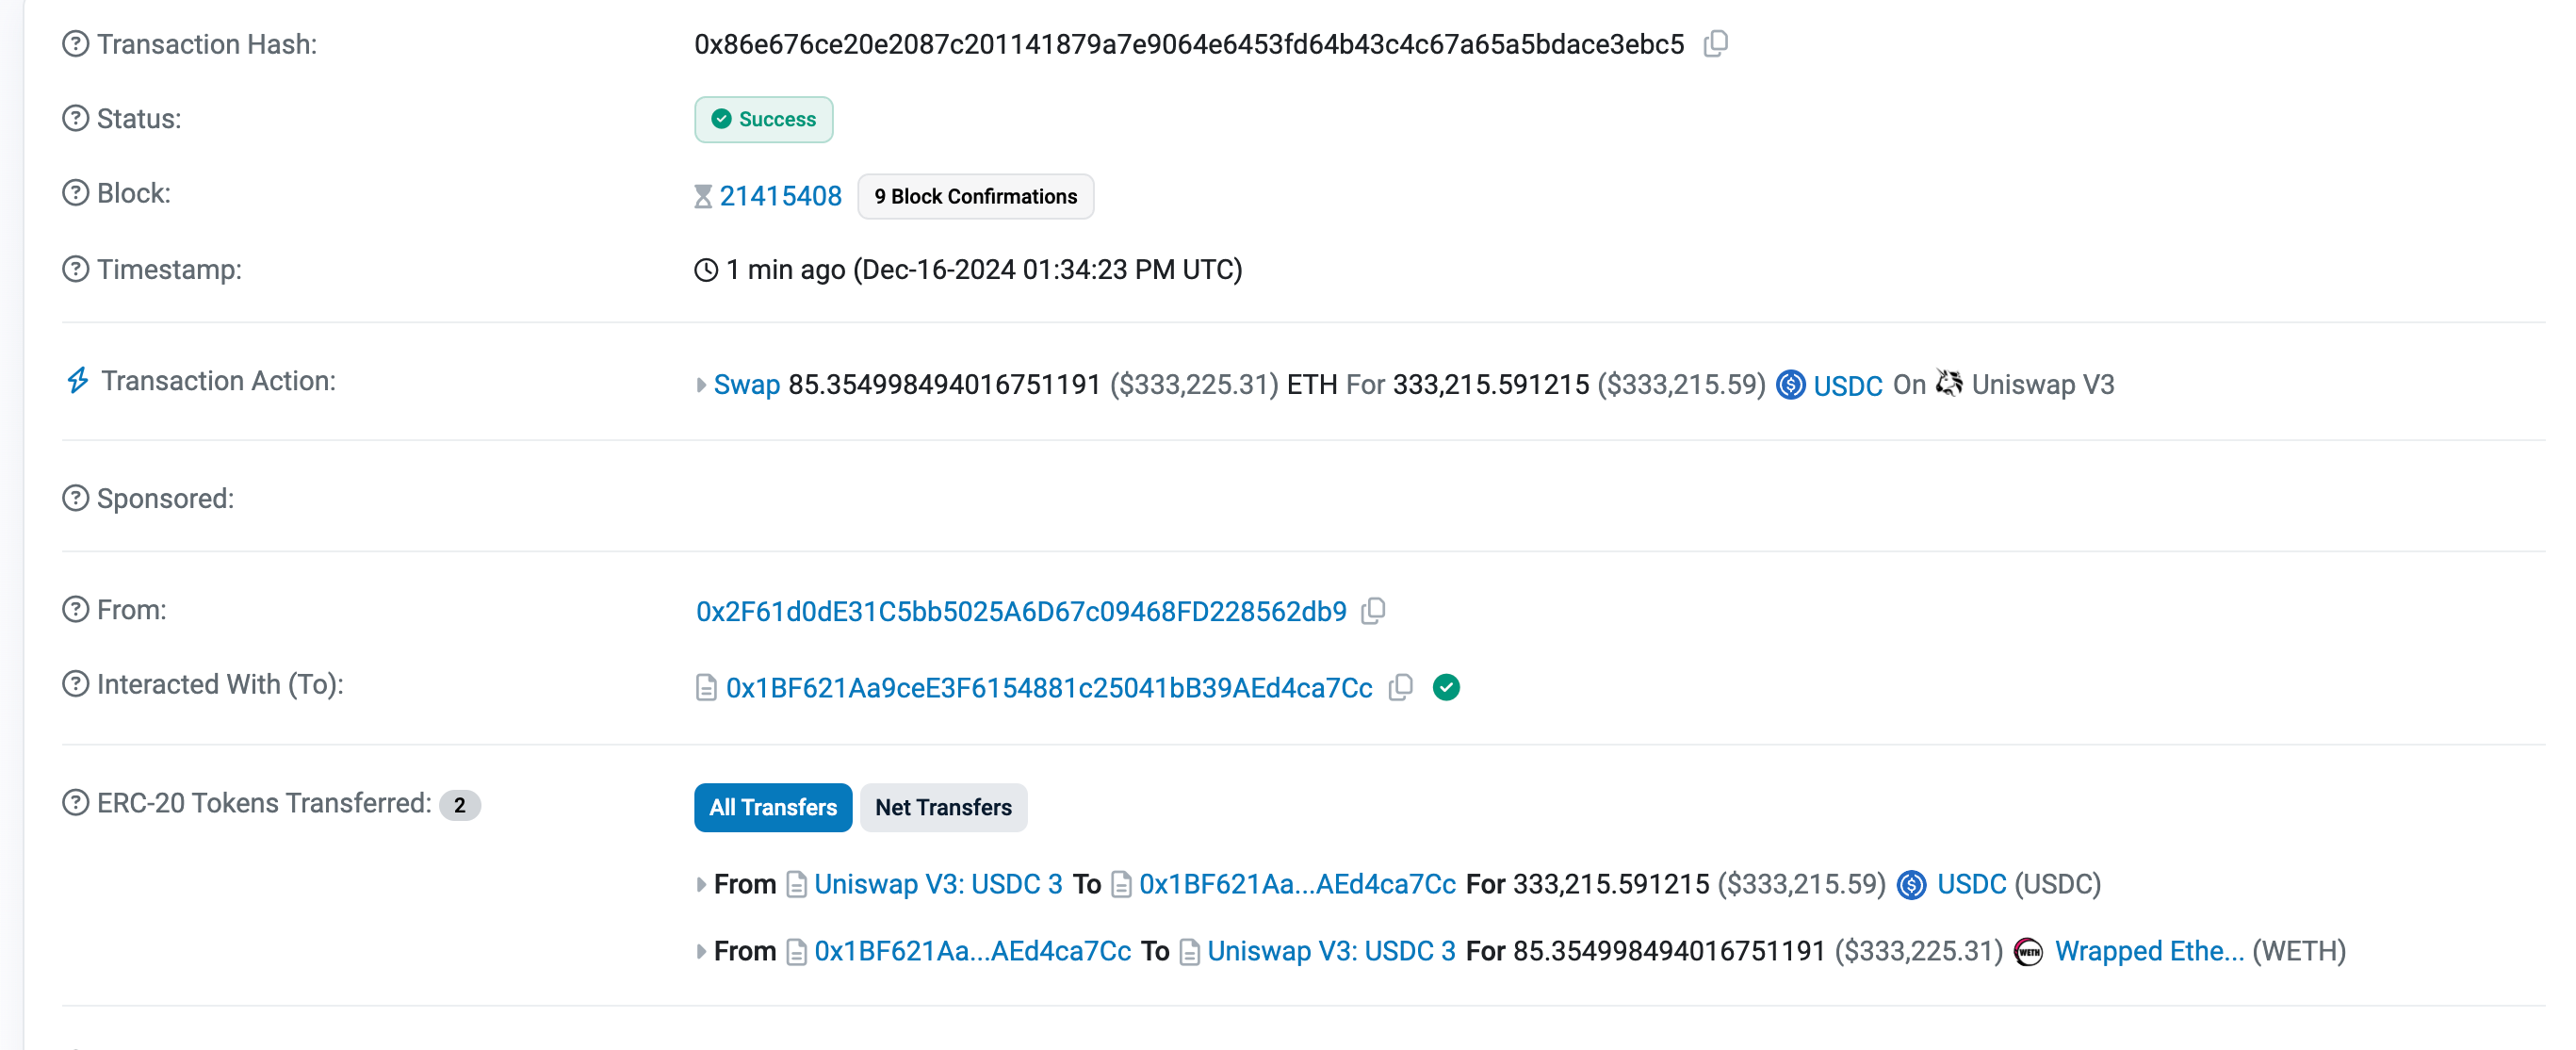
\includegraphics[width=1.0\textwidth]{image/explorers/transaction_swap.png}
    \caption{View a swap transaction in etherscan}
    \label{fig:etherscantx}
\end{figure}

%\begin{figure}[ht]
  %  \includegraphics[width=0.7\textwidth]{image/explorers/otterscan.png}
   % \caption{view a transaction in otterscan}
    %\label{fig:otterscantx}
%\end{figure}




The figures  \ref{fig:logseth} show the same transaction in different explorers: calling the Uniswap V3  usdc-weth LP  to swap tokens; an LP is a Liquidity Pool, the entity which allows to perform tokens swaps by creating a trading pair, as the pair usdc-weth in the figure.  An explorer decodes the data, showing details like token names, transfer amounts, and method names, so users can understand what actions are taking place.


\begin{figure}[ht]
    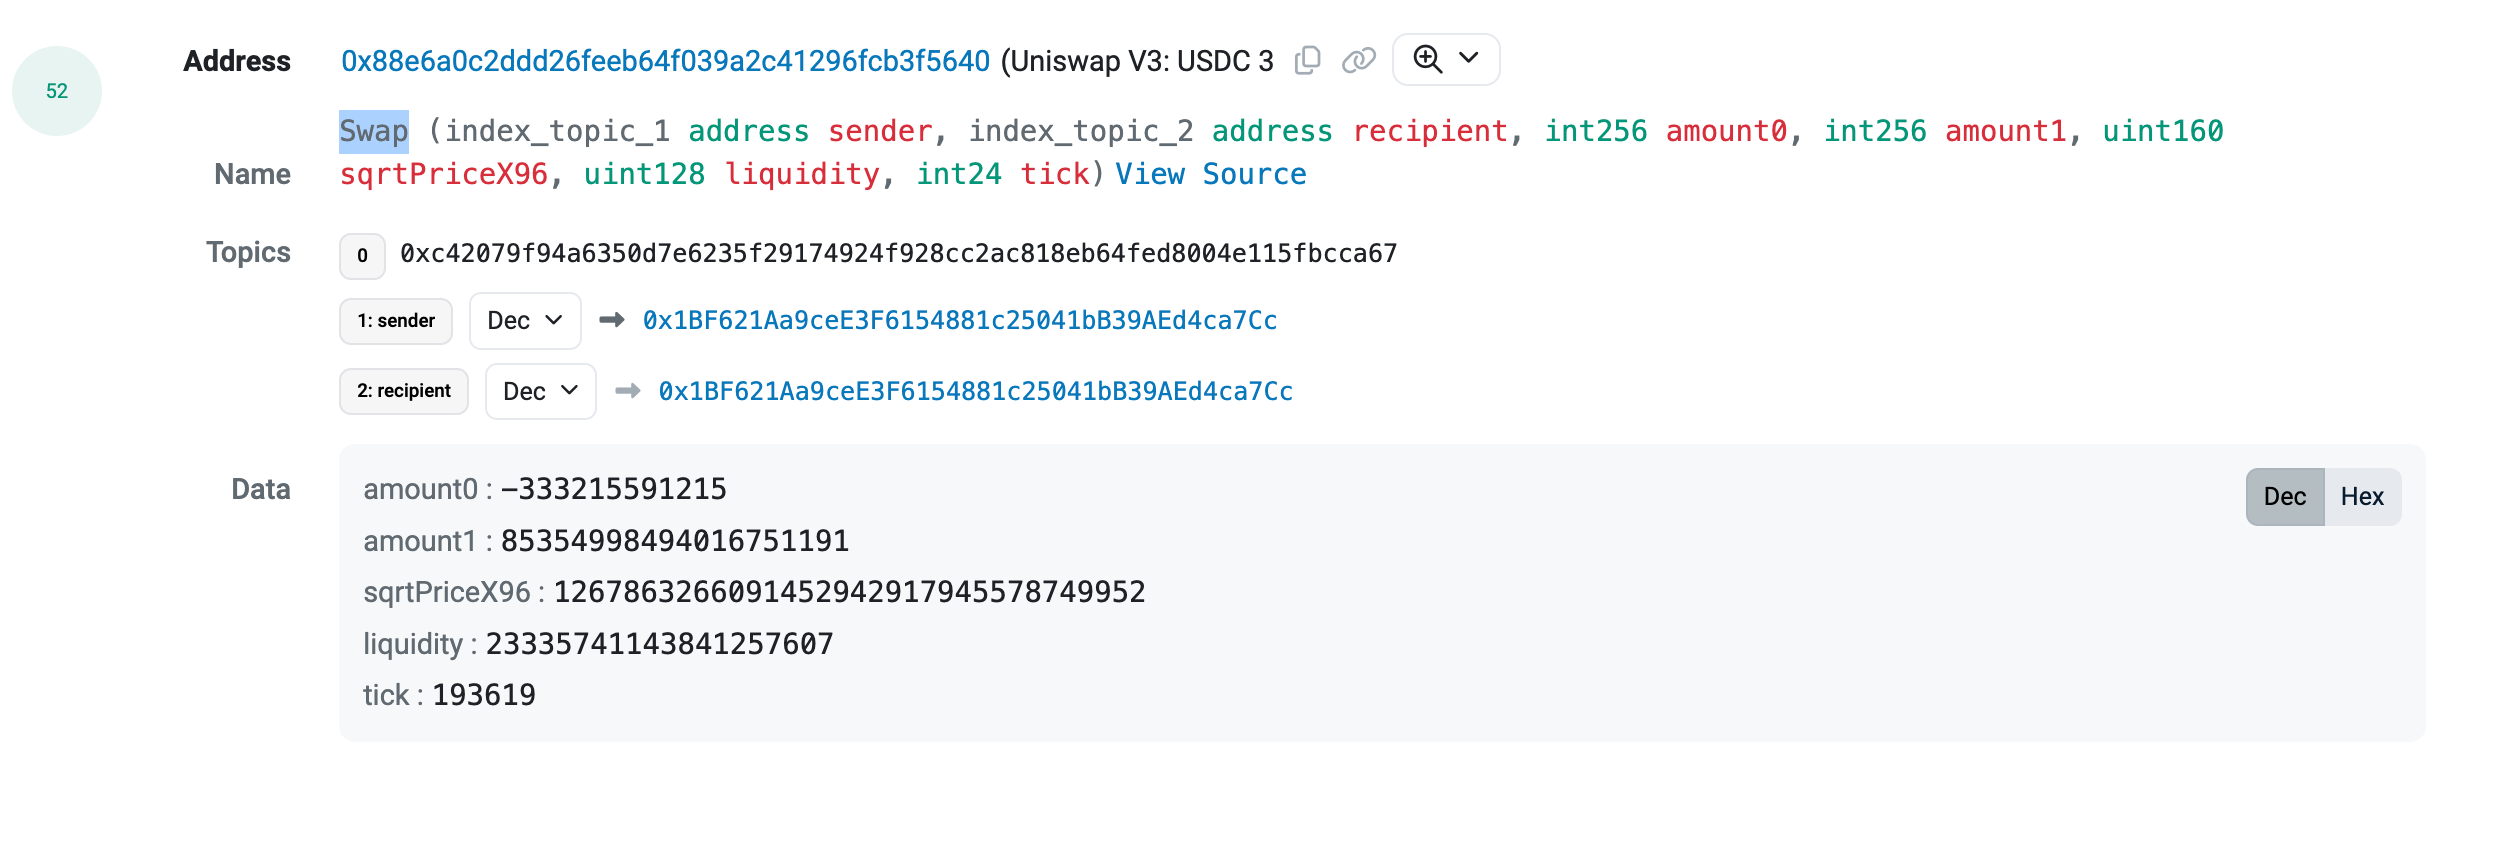
\includegraphics[width=1.0\textwidth]{image/explorers/swapLogs.png}
    \caption{View transaction logs in etherscan}
    \label{fig:logseth}
\end{figure}

The logs view in Etherscan, figure  \ref{fig:logseth}, decodes the event logs emitted by smart contracts during the execution of a transaction, in this case a Uniswap swap.  Without the explorer the swap would appear, as saved in the node database,  like a cryptical string \\
0xc42079f94a6350d7e6235f29174924f928cc2ac818eb64fed8004e115fbcca67 rendered as Topic 0 in the UI. It  represents the Keccak-256 hash of the event’s signature which  is how specific events are identified on the Ethereum blockchain.
In the specific case the string is obtained applying the Keccak-256 hashing to the following signature

\begin{figure}[ht]
\centering
\begin{lstlisting}[basicstyle=\ttfamily, breaklines=true, keepspaces=true, 
                 linewidth=\textwidth, frame=single, escapeinside={\%*}{*}]
Swap(
    address indexed sender,
    uint amount0In,
    uint amount1In,
    uint amount0Out,
    uint amount1Out,
    address indexed to
);
\end{lstlisting}
\caption{Signature of the swap method}
\label{lst:swap_event}
\end{figure}


the full correspondent raw data instead look like a series of encoded hexadecimal strings. 


\begin{figure}[H]
\centering
\begin{lstlisting}[basicstyle=\ttfamily, breaklines=true, keepspaces=true, 
                 linewidth=\textwidth, frame=single, escapeinside={\%*}{*}]
{
  "address": "0xPoolContractAddress",
  "topics": [
    "0xc42079f94a6350d7e6235f29174924f928cc2ac818e
   b64fed8004e115fbcca67", // Swap event signature
    "0xSenderAddress", // Sender (indexed)
    "0xToAddress"      // Recipient (indexed)
  ],
  "data": "0x0000000000000000000000000000000000000
              0000000000000000000005f5e100000000000000
              000000000000000000000000000000000000000
              0000000000000000000000000000000000000000
           000000000000000000000000000000000000989680"
}
\end{lstlisting}
\caption{Logs of the swap method}
\label{lst:swap_event_log}
\end{figure}



\begin{table}[ht]
\centering
\caption{Comparison of Raw Data and Explorer Features}
\begin{tabular}{p{0.45\textwidth}p{0.45\textwidth}}
\hline
\textbf{Raw Data} & \textbf{Explorer} \\ \hline
Raw data logs & Logs presented in a structured and user-friendly format \\ 
Keccak256 hashed method signature & Human-readable method signature \\ 
Indexed parameter values only & Indexed parameter descriptions and values \\ 
Non-indexed data in a unique block in hexadecimal format & Non-indexed data with descriptions and values \\ 
--- & Additional features depending on the explorer \\ \hline
\end{tabular}
\label{tab:raw_vs_explorer}
\end{table}


In general the decoding operation showed above, allowing to present in a human readable format method, parameters and their values,  is done programmatically using a set of rules known as the Ethereum Application Binary Interface (ABI). The ABI defines how to encode and decode function names and parameters for Ethereum smart contracts, allowing a blockchain explorer or other tools to convert raw transaction data into human-readable formats. Several libraries make ABI decoding relatively straightforward, especially for developers building tools or explorers:  web3.js,  ethers.js, Web3.py.
For common contracts like Uniswap or ERC-20 tokens, the ABI files are usually public and can be added to the explorer ABI database, which works like a dictionary where the keccak256 hashes are mapped to the method signature. These ABIs can be used to automatically identify functions and parameters, enabling accurate decoding. Blockchain explorers identify known smart contracts, such as Uniswap in the example above, by using their contract address and displaying relevant details, like contract name and functions. This allows users to recognise trusted contracts versus unknown ones, adding a layer of security when interacting with decentralized finance (DeFi) apps and other dApps.
Explorers like Etherscan and Otterscan can show verified source code and contract metadata (if available) to give insights into the contract’s purpose and functionality.\\
In analysing a transaction sent to a Uniswap contract to perform a token swap the destination address (Uniswap’s contract) and the hex-encoded transaction data (e.g., `0x18cbafe5` followed by more data) couldn’t be interpreted easily. An explorer decodes this, revealing that `0x18cbafe5` maps to `swapExactTokensForTokens` and decodes other parameters, showing token addresses, amounts, and recipient addresses. 
This is particularly beneficials when trying to interprete a flashloan by decoding  the  transactions wrapped between the opening of the loan and its full repayment. The table  \ref{tab:raw_vs_explorer}  shows how the raw data saved in the node client without the help of an explorer or some written ad hoc program would be quite difficult to interprete.




\subsection{Explorer selection}

The explorer selection is a necessary step to deal with the complexity of flashloans. Apart from the de facto standard, which is etherscan, a proprietary close code solution, there are several open-source and free applications that can be installed locally on a self-run Ethereum node. These applications offer functionality similar to Etherscan, the most famous publicly available with limited functionality, including the ability to explore blockchain data, track transactions, and interact with smart contracts. The requirement is to find an implementation well coupled with an Erigon node and with minimal disk requirements and for this  the most known free open source solutions have been analysed.  \\
BlockScout is a versatile and open-source blockchain explorer which supports Ethereum and other Ethereum-compatible networks and can be installed on a local Ethereum node to provide Etherscan-like functionality. \\
Etherchain Explorer is another open-source project that offers blockchain exploration functionality. It's designed to work with Ethereum nodes and provides a web interface to explore blockchain data. \\
Ethereum-ETL is a tool for extracting, transforming, and loading Ethereum blockchain data. While it is more focused on data extraction and transformation, it can be used in conjunction with other tools to build a custom blockchain explorer. \\
Otterscan is a lightweight, open-source Ethereum block explorer embedded in erigon and available as standalone application. All the mentioned explorers, except otterscan require to install an additional DB and rely on ETL to transform chain data and load them in their schema. Otterscan relies on erigon internal mdbx db and, unless instructed differently, uses the erigon indexing process, therefore adding ZERO disk space to the synchronised node. It is especially appealing for developers and researchers who want to avoid reliance on third-party services. Unlike some explorers that require high bandwidth or storage, Otterscan’s design optimizes for performance and fast data retrieval.\\
After some additional test Otterscan and etherscan have prooved to be the best fits: Otterscan to be used in combination with the self hosted node, etherscan to compelment it in certain cases. While Otterscan provides already a complete solution not all the encoded method signatures have been  decoded during the indexing process, on the other hand etherscan seems to be quite complete in this sense but it is proprietary and cannot ensure to give a full access to the full history as required from this paper. Therefore an hybrid solution, having ehterscan as an helper tool has proofed to be the most effective.


\newpage



\section{The Graph protocol}

\subsection{Introduction}

The Graph is an indexing decentralized protocol which adds another dimension to the indexing performed from the node client itself. It is necessary to query in a performant and detailed way specific dApps / protocols like Aave.  In the next sections is presented how the graph addresses the need of an additional process for indexing dApps/protocols data, then is given an overview on the positioning of The Graph in the blockchain landscape  as well as a description of how it works. The last section is dedicated to explain the usage of  The Graph within this paper.


\subsection{Need of indexing the blockchain}

The concept of indexing has been presented  in \ref{bexp:lintro}  in the context of choosing a blockchain explorer accessing indexed data. Indexing is permeating very deeply computer science and can play a role in analysing text documents, classifying documents, speed up searches, minimizing I/O operations or facilitating queries. 


\begin{table}[H] % Use [H] to enforce placement
\centering
\caption{Comparison of Indexing in Computer Science and The Graph Protocol}
\resizebox{\textwidth}{!}{%
\begin{tabular}{lcc}
\toprule
\textbf{Aspect} & \textbf{General Computer Science} & \textbf{The Graph Protocol} \\ 
\midrule
\textbf{Purpose} & Data access optimization & Blockchain data querying \\ 
\textbf{Core Mechanism} & Data structures (trees, hash tables, inverted indexes) & Subgraphs (customized schemas for blockchain data) \\ 
\textbf{Query Language} & SQL, Key-Value lookups, etc. & GraphQL \\ 
\textbf{Data Sources} & Files, databases, memory & Blockchain (e.g., Ethereum, IPFS) \\ 
\textbf{Real-Time Updates} & Not always guaranteed & Enabled via event-driven indexing \\ 
\textbf{Scalability} & Relies on architecture scaling strategies & Decentralized indexing with distributed nodes \\ 
\bottomrule
\end{tabular}%
}
\captionsetup{font=footnotesize, justification=centering}
\caption*{\footnotesize This table compares the roles of indexing in general computer science and The Graph Protocol, highlighting key differences in purpose, mechanisms, and scalability.}
\label{tab:indexing_comparison}
\end{table}

The protocol The Graph cover  an indexing process not addressed  by Erigon: Erigon is actually providing a database general indexing which takes care of the common blockchain query optimisations, as it cannot handle single application data, being this possible only studying in detail the way the app is saving those in the blockchain.
The Graph builds application-specific indexes (subgraphs) tailored to specific needs of decentralized applications (dApps) like summarizing token transfers, aggregating DeFi positions, or fetching NFT metadata; such indexing cannot be done in an abstract  way by a generic blockchain node client, because requires a deep knowledge of the dApp indexed. Leveraging such indexing allows to perform complex queries without having to programmatically process the full chain data or to study the implementation detail of single protocols. It addresses the need of  dApps intercommunication in real time as well as data aggregation offering for it a decentralized network. The last point is important as a centralised usage of single dapps/protocols would neglect the main point of blockchain itslelf: decentralisation. 

\begin{table}[H] % Use [H] to enforce placement
\centering
\caption{Schematic Comparison: Erigon vs. The Graph Protocol}
\resizebox{\textwidth}{!}{%
\begin{tabular}{lcc}
\toprule
\textbf{Aspect} & \textbf{Erigon} & \textbf{The Graph Protocol} \\ 
\midrule
\textbf{Primary Focus} & Raw blockchain indexing & Application-specific indexing \\ 
\textbf{Query Interface} & JSON-RPC, SQL-like queries & GraphQL \\ 
\textbf{Real-Time Updates} & Limited & Event-driven updates \\ 
\textbf{Data Aggregation} & Requires custom implementation & Built-in through subgraphs \\ 
\textbf{Infrastructure} & Self-hosted & Decentralized network \\ 
\textbf{Ease of Use} & Developer-intensive & Plug-and-play for dApps \\ 
\textbf{Use Case} & Blockchain explorers, historical data & dApps requiring structured data \\ 
\bottomrule
\end{tabular}%
}
\captionsetup{font=footnotesize, justification=centering}
\caption*{\footnotesize This table compares Erigon and The Graph Protocol in terms of focus, usability, infrastructure, and support for decentralized applications.}
\label{tab:erigon_vs_graph}
\end{table}


\subsection{Positioning of The Graph. Overview}

The Graph position itself as the google of the blockchains as it allows to efficiently access blockchain data, with the additional advantage of not  relying on centralised services, offering faster and scalable access to information on-chain. Technically The Graph is a decentralised query protocol used for indexing and caching data from blockchains like Ethereum and storage networks. The vision behind The Graph is that Decentralised Applications (dApps) put users in control of their data and to create a wide-scale economic opportunity is needed an interoperability layer between web apps where applications are provided with a common way to query data. The Graph aims to provide a decentralised Query execution Layer for web 3. 

\begin{figure}[ht]
    \centering % Center the image
    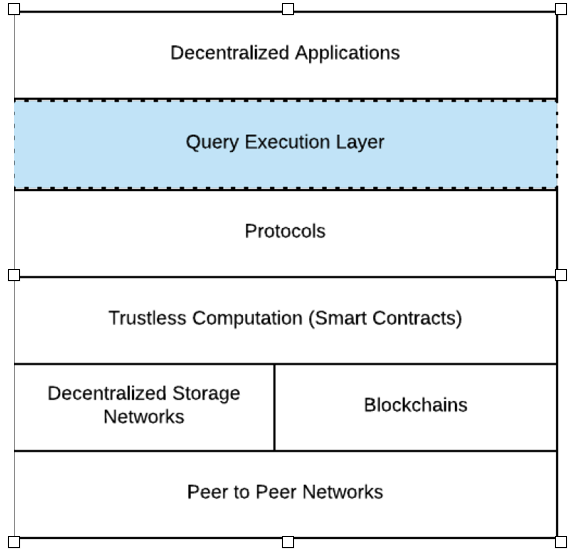
\includegraphics[scale=0.5]{image/thegraph/positioning.png}
    \caption{The Graph in the blockchain landscape}
    \label{fig:thegraphctx}
\end{figure}



\subsection{How The Graph works}
In the official whitepaper is described how The Graph achieves its goals of being a decentralised query execution layer addressing end users, app developers, the graph node operators, data source creators and the graph network validators. Summarising The Graph address indexing by allowing developers to create custom subgraphs, specialized datasets that define what data to extract from the blockchain and how it should be indexed. Once a subgraph is created, it processes new blocks, extracts relevant data, stores them in a relational Db deployed in each The Graph network node and makes it publicly available for querying using GraphQL, an efficient query language.


\subsection{Usage of The Graph}
For the purpose of this paper  providing a subgraph, equivalent of a custom Aave V2 data indexing, is not needed. It would be a difficult operation already covered by reliable and verifiable third parties which, following the protocol rules, are offering a well documented and standardised access to decentralised indexes. Differently from what has been done  for the ethereum itself, setting up a node, no active action of this kind is performed with The Graph. Running a node in The Graph protocol is extremely demanding in term of resources , disk space and network bandwith; it make sense for companies which are setting up a large scale data analysis, selling data, or for some dApps to facilitate the usage of their own protocols in combination with others.  There is actually no need of setting up an ad hoc node or curate the indexing of Aave V2 as the goal is to access data for a specific protocol based on an existing indexing  provided by a reliable curator, for this paper purpose Messari, using the exposed query language, graphql, which constitutes the external layer in front of the data sets which are exposed as REST endpoints. The protocol structure is  transparent and the focus, for this paer purpose, is shifted on the query  usage to get access to meaningful data which facilitate finding interesting flashloans. Messari is specialized in data analytics and provides open source data indexing of various blockchain leveraging The Graph, adding data presentation and deployment automatisation stategies. 
Owning an ethereum node allows to use the extracted data and countercheck their validity in combination with a blockchain explorer.

\begin{figure}[ht]
    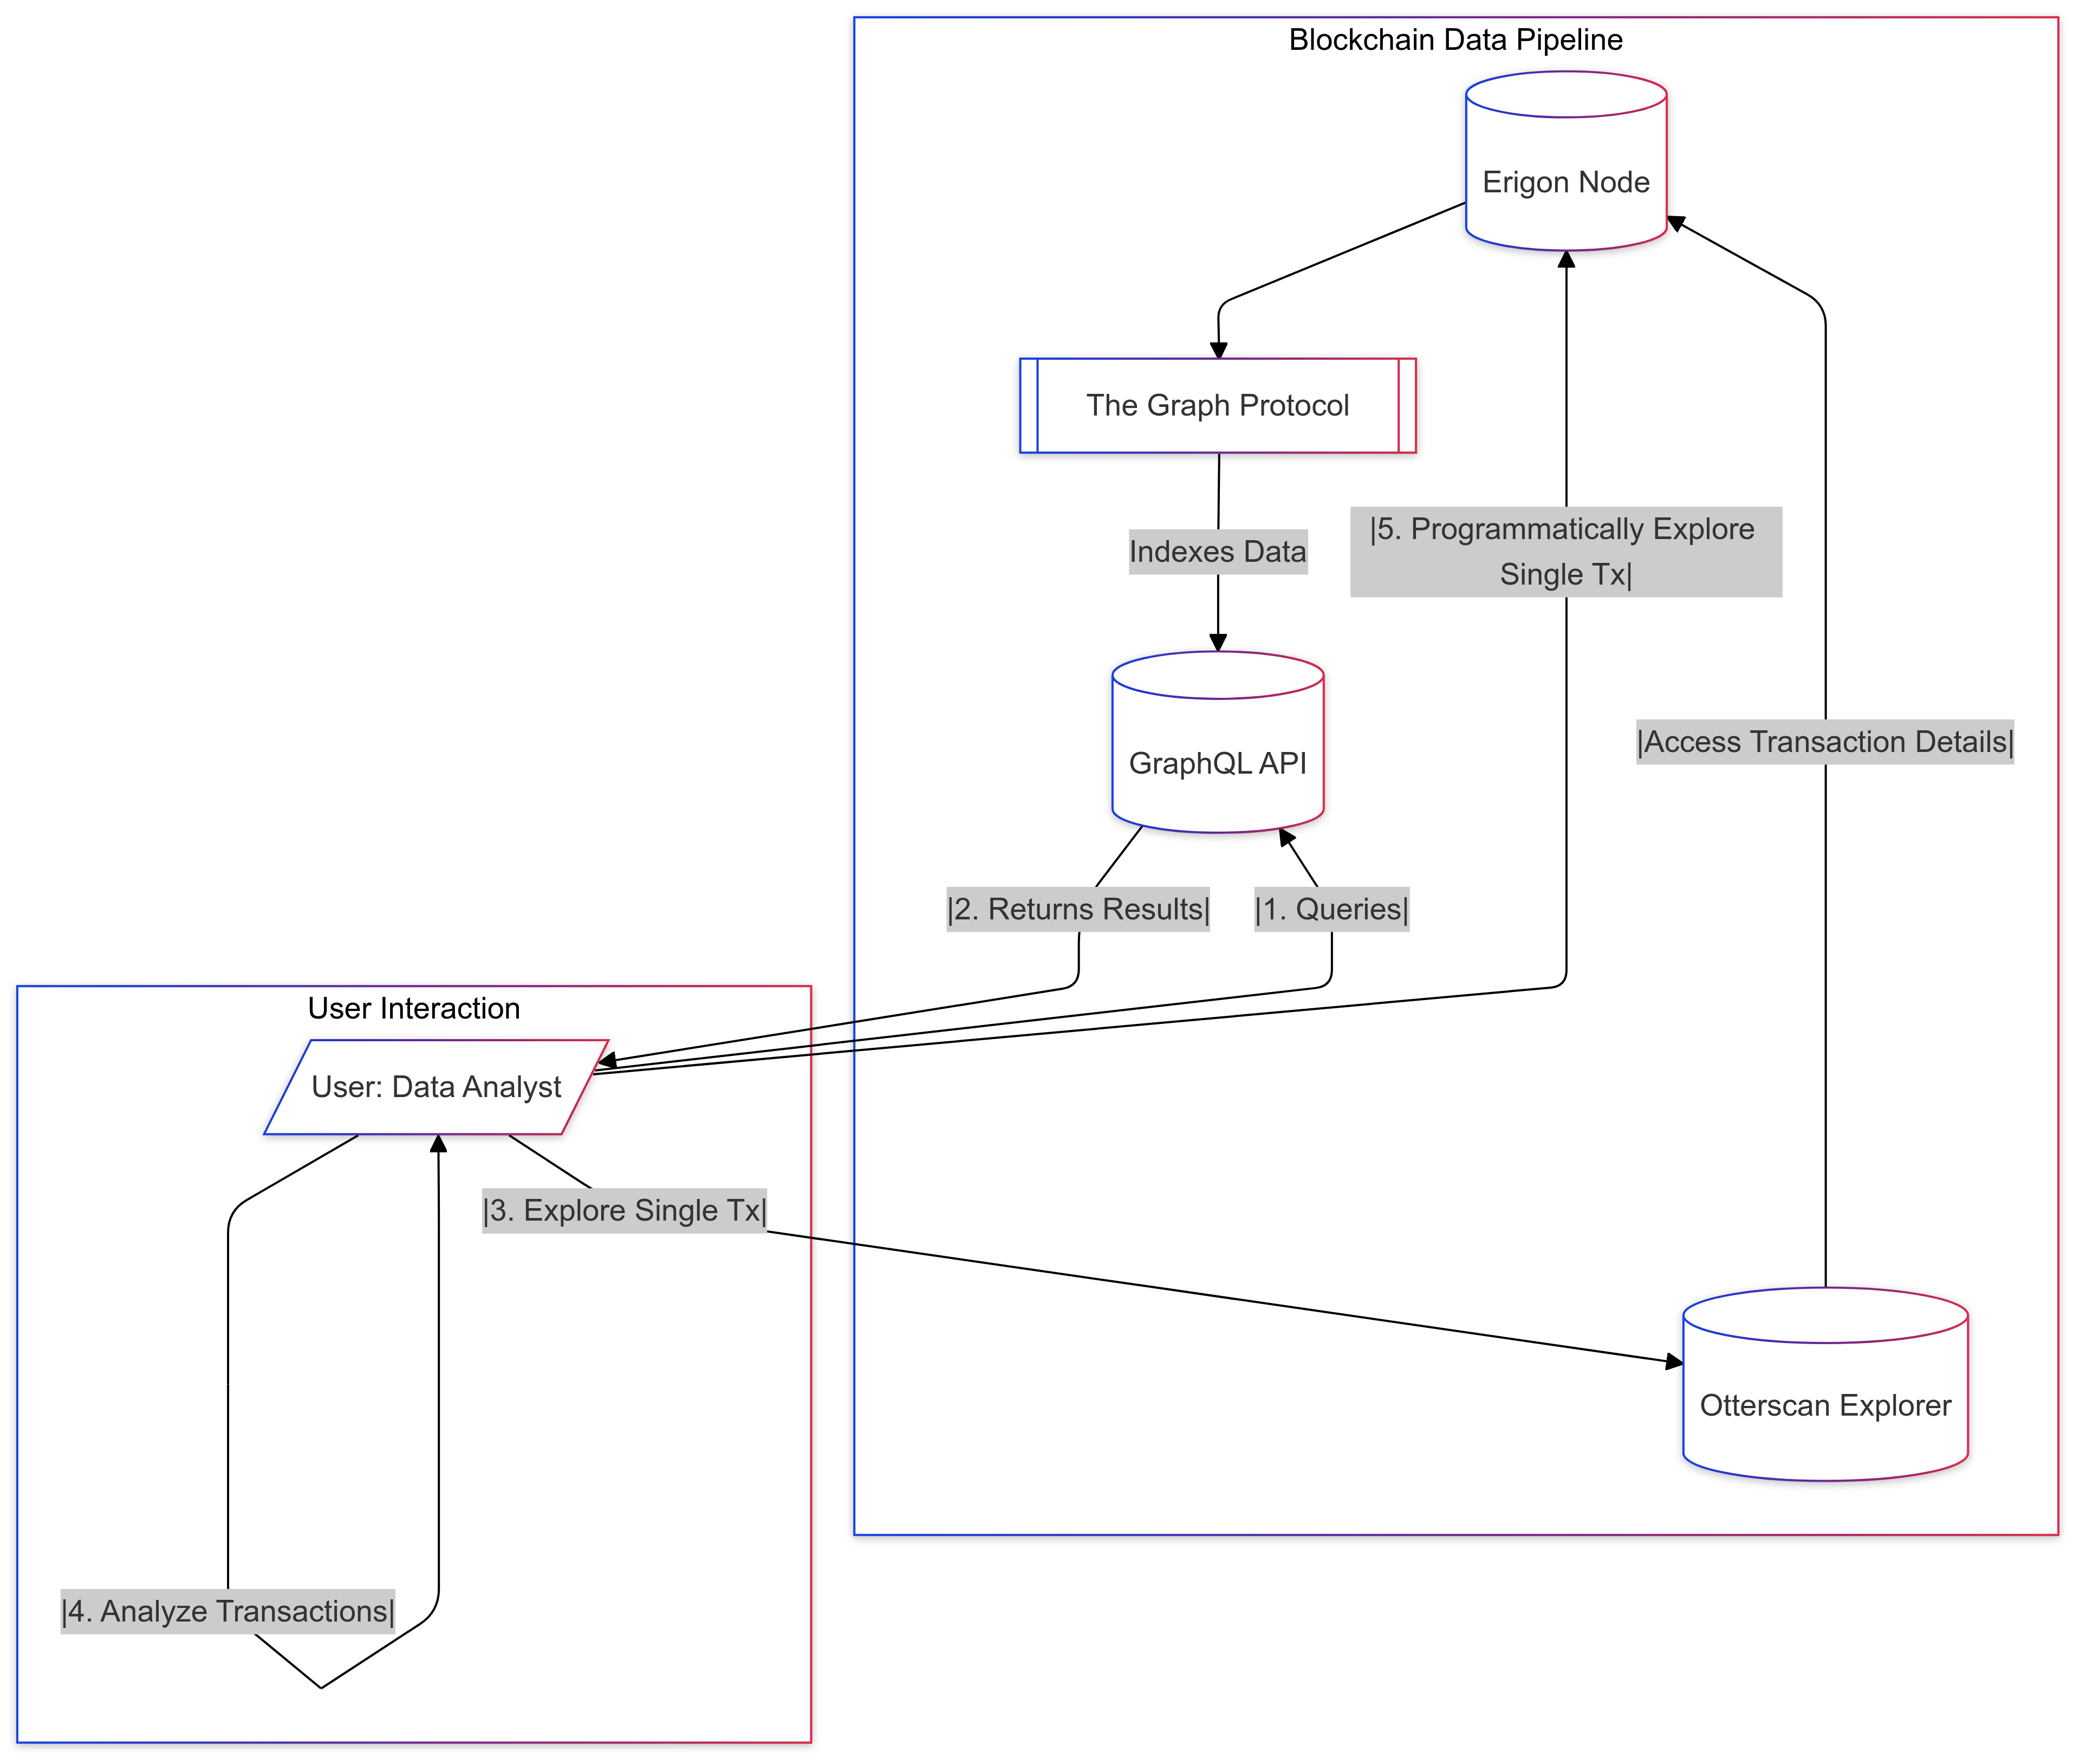
\includegraphics[width=1.0\textwidth]{image/thegraph/process.png}
    \caption{Usage of the graph in combination with erigon node and otterscan}
    \label{fig:processthegraph}
\end{figure}

This paper leverages The Graph exposed endpoints for indexed Aave V2 data. The approach is to send different requests to filter data which facilitate further investigation. In presenting possible usage of flashloans, without a criterion to select potential arbitrages, or protocol attacks (literally hacking of protocol financed through flashloans) or collateral swapping would be almost impossible to find significant transitions without processing all the flashloans calls and examining them punctually. This is a colossal challenge as a flashloan is often wrapping plenty of transactions, even hundreds. An heuristic approach like selecting the largest 20 flashloans issued since inception assuming they will be used for an arbitrage or for hacking a protocol increases the probability of finding such transactions. A blockchain explorer helps in their analysis afterwards. This suggest  that an effective pattern of work consists in using in the following order The Graph, a blockchain scanner, otterscan/etherscan or direct queries on the node like erigon api calls if needed. The graph queries with less restrictive filters provide bulk exports of data which could be used to perform statistical analysis as flashloans usage on time by account type and size.
The Graph itself  runs on Arbitrum , an L2 chain chosen for low gas cost solution, as indexing service. The indexed data are selected from the proper chain, ethereum,  stored through mappers in a db and exposed as already explained. Arbitrum is just a convenient solution for the protocol management.

\begin{table}[H] % Use [H] to enforce placement
\centering
\caption{Summary: Leveraging The Graph for Aave V2 Flashloan Analysis}
\resizebox{\textwidth}{!}{%
\begingroup
\fontsize{8.5}{10}\selectfont % Reduces character size by approximately 15%
\begin{tabular}{|l|p{12cm}|}
\hline
\textbf{Aspect} & \textbf{Details} \\ 
\hline
\textbf{Purpose} & Utilize The Graph endpoints to index and filter Aave V2 data for analysis of flashloans and related activities. \\ 
\hline
\textbf{Challenge} & Analyzing flashloans is complex due to their wrapping of multiple transactions (sometimes hundreds), making it hard to identify significant patterns without processing all calls. \\ 
\hline
\textbf{Potential approach} & 
Use The Graph for bulk data extraction with less restrictive filters.  
Apply heuristics (e.g., focus on the largest 20 flashloans) to narrow the scope.  
Analyze selected transactions using blockchain explorers (e.g., Otterscan/Etherscan) or direct node queries (e.g., Erigon API). \\ 
\hline
\textbf{Insights Enabled} & 
Statistical analysis of flashloan usage over time by account type and size.  
Identification of potential arbitrages, protocol attacks, or collateral swaps. \\ 
\hline
\textbf{Infrastructure} & 
- \textbf{The Graph}: Queries indexed data from Ethereum and exposes it via endpoints.  
- \textbf{Arbitrum}: Used as a low-cost Layer 2 solution for managing The Graph's indexing service. \\ 
\hline
\textbf{Workflow Pattern} & 
Query data using The Graph.  
Perform detailed analysis with blockchain scanners or direct node queries if needed. \\ 
\hline
\end{tabular}%
\endgroup
}
\captionsetup{font=footnotesize, justification=centering}
\caption*{\footnotesize This table summarizes the approach and workflow for leveraging The Graph to analyze Aave V2 flashloan data, including infrastructure, challenges, and insights gained.}
\label{tab:flashloan_analysis}
\end{table}


\subsection{The Graph: technical view}

To understand how The Graph works under the hood is useful a simplified example of creating, deploying  and indexing a subgraph. After this is done it is possible to query the indexed data according to the defined interface. The steps consist in defining the subgraph.yaml, writing a mapper from blockchain data to indexed data telling how to transform and to save them in the db (at the moment a postgresql db), define the query language through GraphQL schema, deploying the subgraph, signalling to indexers to start to process it and finally having the data available to be queried by end users. In this paper the only step directly performed is \textbf{\textit{Querying}} the proper subgraph. This section explains what The Graph protocols and actors (curators and indexers) do to allow to run queries on a subgraph.

\begin{table}[H]
\centering
\caption{Schematic Summary of Subgraph Workflow in The Graph}
\resizebox{\textwidth}{!}{%
\begin{tabular}{|l|l|}
\hline
\textbf{Step} & \textbf{Description} \\ \hline
\textbf{Prerequisites} & Install Node.js, Yarn, and Graph CLI for subgraph management. \\ \hline
\textbf{Define Subgraph} & Create `subgraph.yaml` specifying network, contract address, events, and mapping files. \\ \hline
\textbf{Mapping Handlers} & Use AssemblyScript to process blockchain events into database-storable format. \\ \hline
\textbf{GraphQL Schema} & Define data structure for querying (e.g., entities like transfers). \\ \hline
\textbf{Deploy Subgraph} & Deploy the subgraph using `graph deploy` command to a hosted service or decentralized network. \\ \hline
\textbf{Indexing} & Indexers, incentivized by curators staking GRT, process and store the data. \\ \hline
\textbf{Querying} & Query indexed data using GraphQL (e.g., retrieve transfers sorted by value). \\ \hline
\end{tabular}%
}
\captionsetup{font=footnotesize, justification=centering}
\caption*{\footnotesize This table outlines the main steps for creating, deploying, indexing, and querying a subgraph in The Graph ecosystem.}
\label{tab:subgraph_workflow}
\end{table}

\textbf{\textit{Technical prerequisites}}
\begin{lstlisting}[language=bash, caption={Installation Commands for Subgraph Setup}, label={lst:install_commands}, basicstyle=\ttfamily\scriptsize]
# Install Node.js and Yarn (package managers for JavaScript)
# Install Graph CLI, a command-line tool to generate and manage subgraphs
npm install -g @graphprotocol/graph-cli
\end{lstlisting}



\textbf{\textit{Define the Subgraph}}

The process begins by defining a subgraph that specifies which events, functions, or data  to index from the blockchain. It is needed to provide a Subgraph Manifest as a YAML file (called `subgraph.yaml`) where you define your subgraph by including the network (Ethereum, Polygon, etc.), the contract addresses you're tracking and the specific smart contract events or functions to index.

\begin{lstlisting}[language=xml, caption={Example subgraph.yaml}, label={lst:subgraph_yaml}, basicstyle=\ttfamily\scriptsize]
specVersion: 0.0.2
description: Example subgraph
schema:
  file: ./schema.graphql
dataSources:
  - kind: ethereum/contract
    name: MyContract
    network: mainnet
    source:
      address: "0x123...abc"
      abi: MyContract
      startBlock: 12345678
    mapping:
      kind: ethereum/events
      apiVersion: 0.0.5
      language: wasm/assemblyscript
      entities:
        - MyEntity
      abis:
        - name: MyContract
          file: ./abis/MyContract.json
      eventHandlers:
        - event: Transfer(indexed address, indexed address, uint256)
          handler: handleTransfer
      file: ./src/mapping.ts
\end{lstlisting}
   

\textbf{\textit{Write the Mapping Handlers}}

Mapping handlers are written in AssemblyScript and define how to process specific blockchain events. When the specified event occurs, the handler transforms it into a format that can be stored in the subgraph (saving it in a database).


\begin{lstlisting}[language=xml, caption={Example handler for a Transfer event}, label={lst:transfer_handler}, basicstyle=\ttfamily\scriptsize]
import { Transfer } from '../generated/MyContract/MyContract'
import { MyEntity } from '../generated/schema'

export function handleTransfer(event: Transfer): void {
  let entity = new MyEntity(event.transaction.hash.toHex())
  entity.from = event.params.from
  entity.to = event.params.to
  entity.value = event.params.value
  entity.save()
}
\end{lstlisting}
  

This code defines how to extract event parameters (`from`, `to`, `value`) and store them in the subgraph.

\textbf{\textit{Define the GraphQL Schema}}

The schema defines how the data should be structured and queried. It is what the end user will call.


\begin{lstlisting}[language=xml, caption={Example GraphQL Schema}, label={lst:graphql_schema}, basicstyle=\ttfamily\scriptsize]
type MyEntity @entity {
  id: ID!
  from: Bytes!
  to: Bytes!
  value: BigInt!
}
\end{lstlisting}
 

This GraphQL schema defines the structure of the entity (e.g., transfers) you’re indexing from the blockchain.

\textbf{\textit{Deploy the Subgraph}}
After defining the subgraph and handlers, deploy the subgraph to The Graph’s decentralized network or hosted service using:

\begin{lstlisting}[language=bash, caption={Graph Deploy Command}, label={lst:graph_deploy}, basicstyle=\ttfamily\scriptsize]
graph deploy --node https://api.thegraph.com/deploy/ <your-subgraph-name>
\end{lstlisting}
 
\textbf{\textit{Indexing}}
After deployng, the job of the curator role is finished. The data are not yet available to be queried. Somebody has to index the data. This is the role of the Indexer which are incentivised to participate by the curators themselves. A curator stake some native token, GRT, and broadcasts a signal in the network. Indexers are compensated with these GRT for their work and the resources they make available.

\textbf{\textit{Querying}}
Once the subgraph is indexed, the end user can query it using GraphQL which allows to request specific data efficiently.

\begin{lstlisting}[language=xml, caption={Query for the Top 5 Token Transfers Sorted by Value}, label={lst:query_transfers}, basicstyle=\ttfamily\small]
{
  myEntities(first: 5, orderBy: value, orderDirection: desc) {
    from
    to
    value
  }
}
\end{lstlisting}


This query retrieves the 5 largest "myEntities" from the subgraph deployed  sorted by value.


\newpage

\section{Data analysis process}

\subsection{Introduction}
The previous  chapters present the main protocol studied in this work and the tools which allow to perform data analysis on it. 
The process followed is quite standardised and this chapter shows how it works in a general way 

\subsection{Analysis Tools}
The Graph allows to identify a set of potential interesting flashloans by querying via graphql the Messari subgraph. The request criteria sent to the public interface can be different depending on the analysis which is addressed. In this section the methodology is presented in general and an example is provided. Once a set of parameters has been decided the output from graphql can be analysed in various ways. A query can return a bulk amount of data, for example last 5000 flashloans, and the analysis can just focus on the returned data, by sorting and classifing them: this need a good data analysis toolbox, typically python and its rich data analysis and presentation libraires. Another informative approach is setting up criteria which are likely to isolate few trades, therefore returning a limited number of results, and study them in detail. For example a query can select flashloans which were presenting a profit when closed, sorted from the largest and picking the top 10, or count flashloans by month since inception and study  correlations between this number and variables as ethereum gas price or ethereum price itself to mention some.  This paper relies on the  approach of selecting few meaningful trades and analyse them. 
Once the flashloans are selected, the blockchain explorer and the local node role becomes relevant as the single transactions need  to be checked in details.
Selecting the top 10 largest flashloans gives five different use cases which are presented in dedicated chapters. 

\subsection{Transaction list}

This section present an example of query to the Messari subgraph. Technically this means that Messari, as curator, has defined a subgraph to index and persist the Aave V2 data and an interface to query them and indexers have picked up the task of actually processing the subgraph exposing it to the general public. 
The graphql service is exposed via https at \\

\texttt{https://thegraph.com/explorer/subgraphs/\break
C2zniPn45RnLDGzVeGZCx2Sw3GXrbc9gL4ZfL8B8Em2j?\break
view=Query\&chain=arbitrum-one}

\begin{figure}[ht]
    \centering % Center the image
    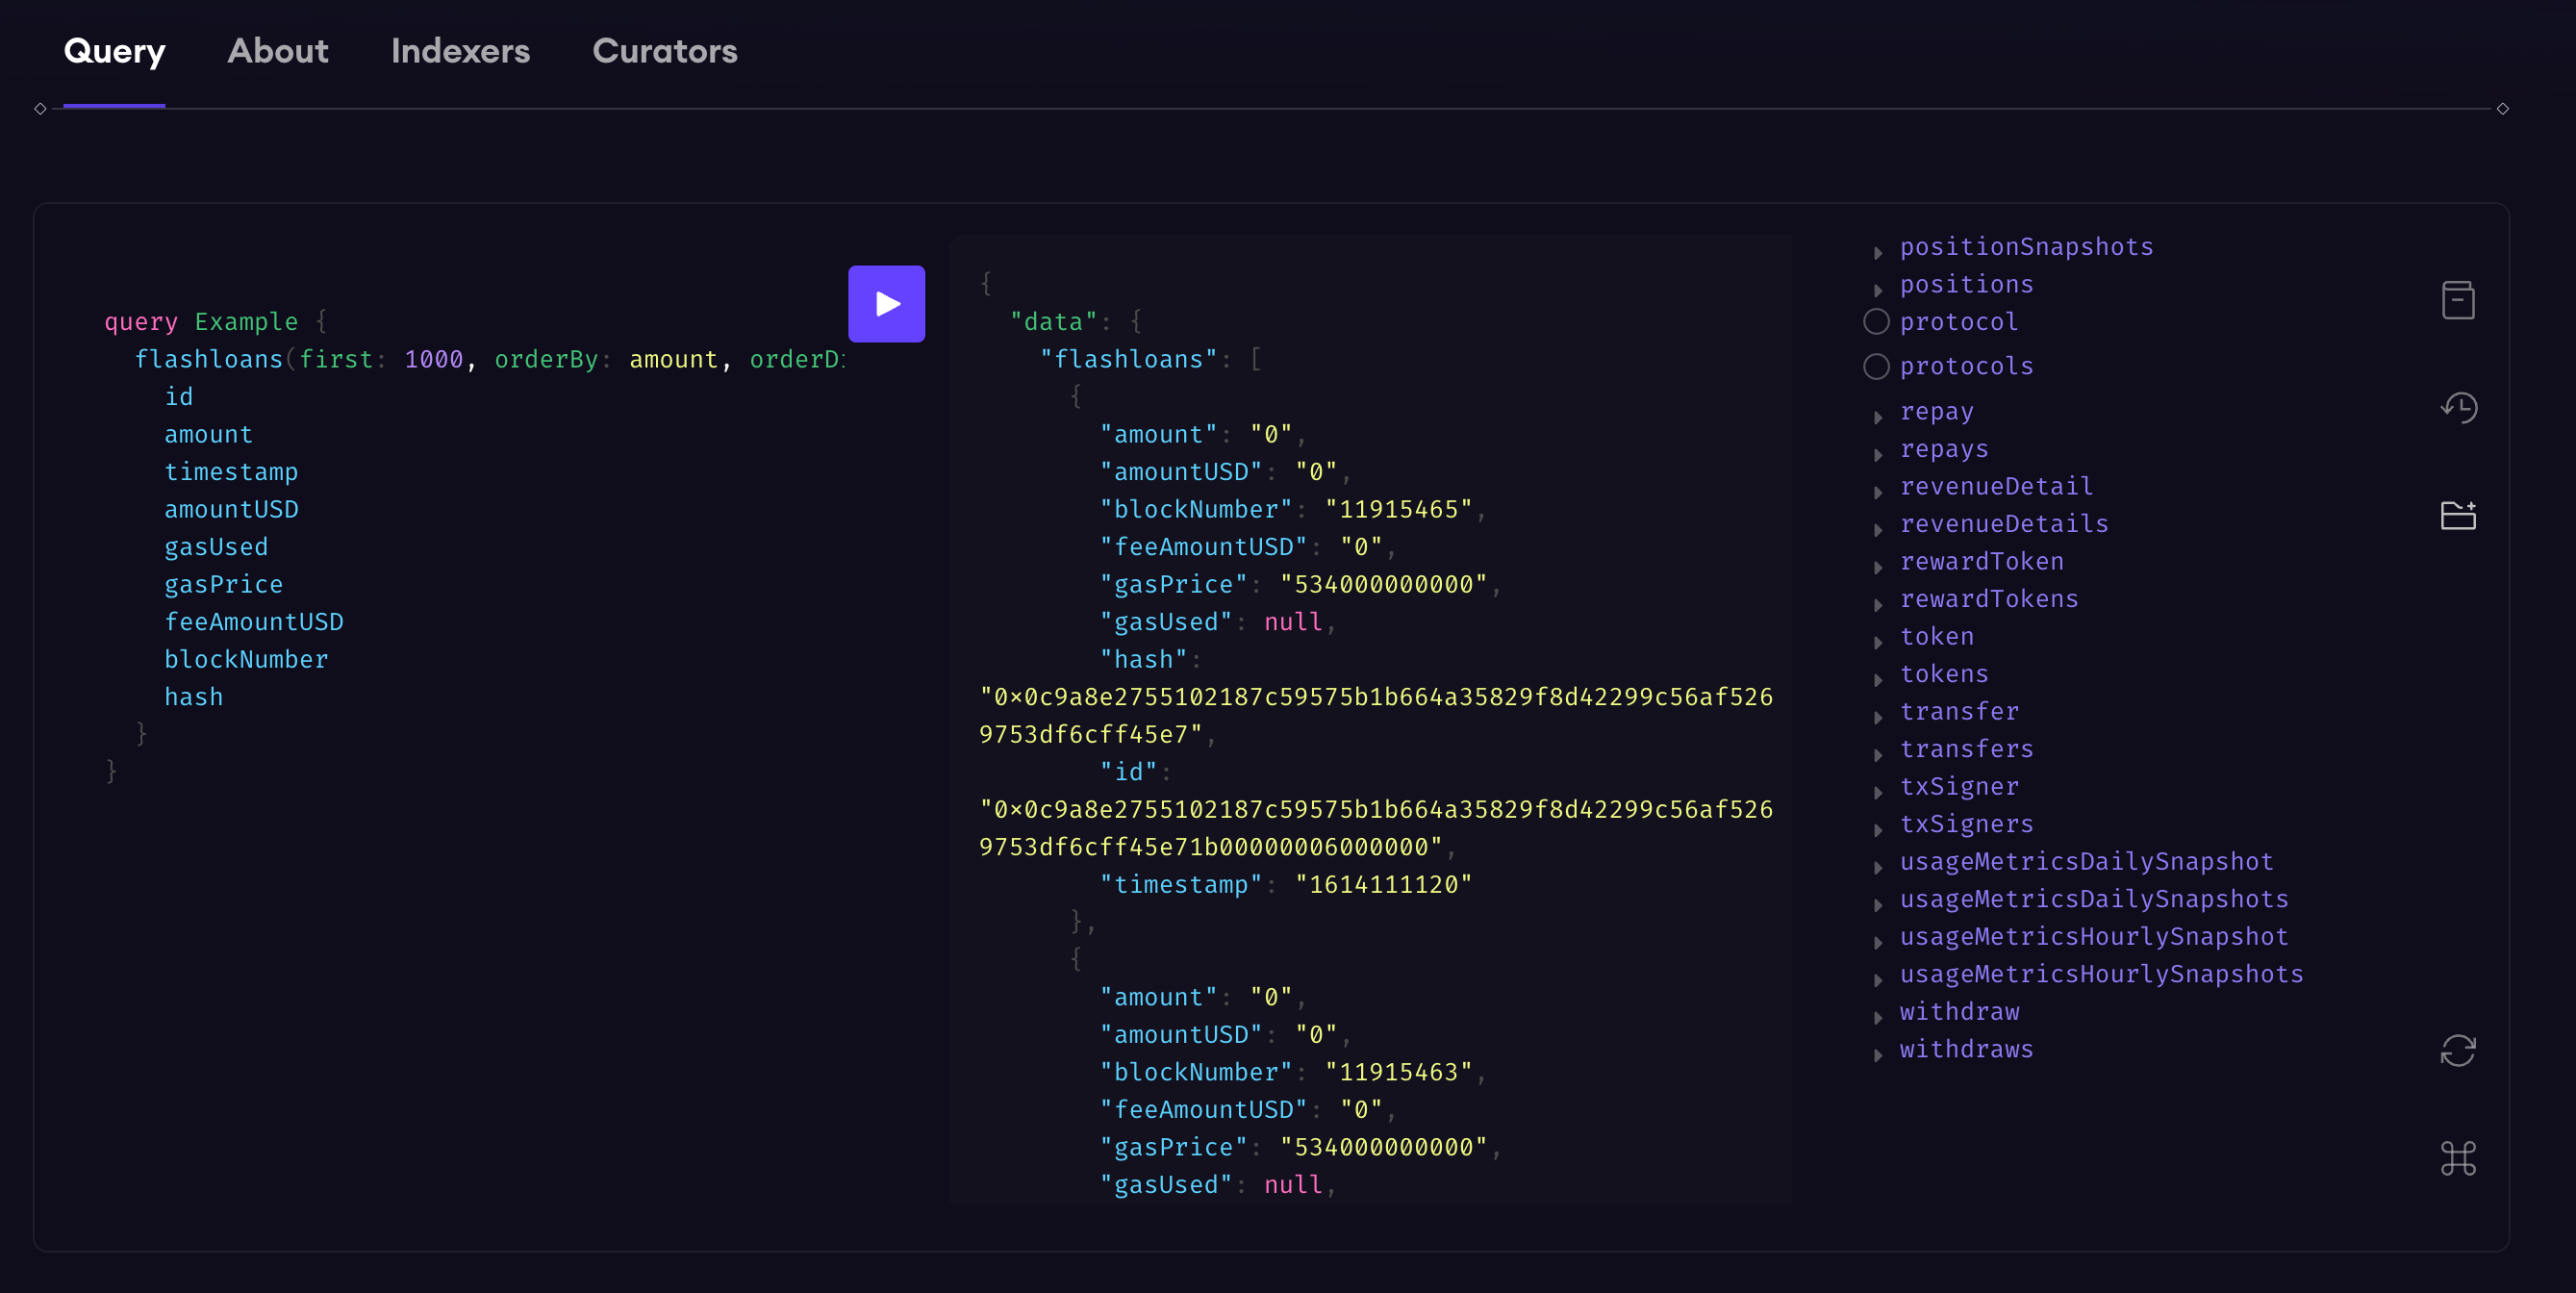
\includegraphics[width=\textwidth]{image/process/messari.png} % Scale image to fit the text width
    \caption{Messari Aave V2 Interface}
    \label{fig:aavemessari}
\end{figure}

\vspace{0.5cm} % Adds some space between figure and listing

the figure \ref{fig:aavemessari} show the request in this example on the left side, the response in the center and the possible parameters on the right. A query can be composed and tested  on line using this  right side schema. The schema are providing in yaml format, a common standard, which allows in every main development language to rely on code generators to eventually access the endpoint programmatically.\\
The request sent:


\begin{lstlisting}[language=xml, caption={Example JSON request for flashloans}, label={lst:fl_example}, basicstyle=\ttfamily\scriptsize]
{
  flashloans(first: 1000, orderBy: amount, orderDirection: desc) {
    id
    amount
    timestamp
    amountUSD
    gasUsed
    gasPrice
    feeAmountUSD
    blockNumber
    hash
  }
}
\end{lstlisting}
  

The response, which include 1000 entries, can be processed programmatically or analysed punctually depending on the goal. Ordering by gasPrice or gasUsed shows  another criterion to extract value from the same query.


For the purpose of this paper the following query has allowed to extract all the meaningful transactions.

\begin{lstlisting}[language=xml, caption={ JSON request for top 10  usd amount flashloans }, label={lst:fl_topten}, basicstyle=\ttfamily\scriptsize]
{
  flashloans(first: 10, orderBy: amount, orderDirection: desc) {
    id
    amount
    timestamp
    amountUSD
    blockNumber
    hash
  }
}
\end{lstlisting}


\begin{lstlisting}[language=xml, caption={ JSON response for top 10 usd amount flashloans}, label={lst:fl_topten_rsp}, basicstyle=\ttfamily\scriptsize]
{
  "data": {
    "flashloans": [
      {
        "amount": "350000000000000000000000000",
        "amountUSD": "349597751.4474315409598895928248957",
        "blockNumber": "14602790",
        "hash": "0xcd314668aaa9bbfebaf1a0bd2b6553d01dd58899c508d4729fa7311dc5d33ad7",
        "id": "0xcd314668aaa9bbfebaf1a0bd2b6553d01dd58899c508d4729fa7311dc5d33ad76900000006000000",
        "timestamp": "1650198256"
      },
      {
        "amount": "78465988600582788297000000",
        "amountUSD": "78488458.63395031958301255403372147",
        "blockNumber": "12765761",
        "hash": "0x7567551456d5bafc6816e40b3dfa27de4040d140430c7d815e641d301755fb0b",
        "id": "0x7567551456d5bafc6816e40b3dfa27de4040d140430c7d815e641d301755fb0b3001000006000000",
        "timestamp": "1625464917"
      },
      {
        "amount": "77926704000000000000000000",
        "amountUSD": "78097069.42128388169628392697528458",
        "blockNumber": "12428389",
        "hash": "0xa55285d2d43562befbc4d2e76e722f4e34973a42cfe9f40b5222bf0f68bb8841",
        "id": "0xa55285d2d43562befbc4d2e76e722f4e34973a42cfe9f40b5222bf0f68bb8841a500000006000000",
        "timestamp": "1620939686"
      },
      {
        "amount": "50000000000000000000000000",
        "amountUSD": "30444198.7266429157239672265873159",
        "blockNumber": "17845588",
        "hash": "0x006763dff653ecddfd3681181a29e7e6d6c2aaa7bafb27fe1376f3f7ce367c1e",
        "id": "0x006763dff653ecddfd3681181a29e7e6d6c2aaa7bafb27fe1376f3f7ce367c1ea102000006000000",
        "timestamp": "1691200055"
      },
      {
        "amount": "38100000000000000000000000",
        "amountUSD": "38342882.139495868976566678826281",
        "blockNumber": "15937667",
        "hash": "0x04c43669c930a82f9f6fb31757c722e2c9cb4305eaa16baafce378aa1c09e98e",
        "id": "0x04c43669c930a82f9f6fb31757c722e2c9cb4305eaa16baafce378aa1c09e98e1000000006000000",
        "timestamp": "1668059735"
      },
      {
        "amount": "30000000000000000000000000",
        "amountUSD": "29932733.02152474596203285671482896",
        "blockNumber": "16817996",
        "hash": "0xc310a0affe2169d1f6feec1c63dbc7f7c62a887fa48795d327d4d2da2d6b111d",
        "id": "0xc310a0affe2169d1f6feec1c63dbc7f7c62a887fa48795d327d4d2da2d6b111d3700000006000000",
        "timestamp": "1678697459"
      },
      {
        "amount": "17785000000000000000000000",
        "amountUSD": "10536802.08457644928766999449880354",
        "blockNumber": "17903042",
        "hash": "0x9dd926678b0a75a9448a158fd5a3dba613f65372eb0f137e038f89ba8c891435",
        "id": "0x9dd926678b0a75a9448a158fd5a3dba613f65372eb0f137e038f89ba8c8914353f02000006000000",
        "timestamp": "1691894771"
      },
      {
        "amount": "17510000000000000000000000",
        "amountUSD": "17550472.16590467174269099446059612",
        "blockNumber": "17620871",
        "hash": "0xdd7dd68cd879d07cfc2cb74606baa2a5bf18df0e3bda9f6b43f904f4f7bbdfc1",
        "id": "0xdd7dd68cd879d07cfc2cb74606baa2a5bf18df0e3bda9f6b43f904f4f7bbdfc17800000006000000",
        "timestamp": "1688477447"
      },
      {
        "amount": "13708154106140136718749954",
        "amountUSD": "13702180.60459149942423018167739925",
        "blockNumber": "13728544",
        "hash": "0xd59e11e7e078332e145fd9981507e3286c5f6aedcda93469c6ae3af46f5cdfe6",
        "id": "0xd59e11e7e078332e145fd9981507e3286c5f6aedcda93469c6ae3af46f5cdfe61b02000006000000",
        "timestamp": "1638464665"
      },
      {
        "amount": "7216185760498046874999928",
        "amountUSD": "7255611.580116158337753218219719296",
        "blockNumber": "13950121",
        "hash": "0x28532551bd89fb15cc56941ed367596aeb63fabd492100d53b3896b7ad9d5ce5",
        "id": "0x28532551bd89fb15cc56941ed367596aeb63fabd492100d53b3896b7ad9d5ce58200000006000000",
        "timestamp": "1641448505"
      }
    ]
  }
}
\end{lstlisting}

\newpage

\section{Selected flashloans use cases}

This chapters describes the different use cases of Flashloans included in the transactions presented in the listing \ref{lst:fl_topten_rsp}  

\subsection{Beanstalk protocol hack}

The transaction 0xcd314668aaa9bbfebaf1a0bd2b6553d01dd58899c508d4729fa7311dc5d33ad7 is the greatest flashloan ever issued. It was used for hacking Beanstalk a decentralised protocol.
The transaction 0xc310a0affe2169d1f6feec1c63dbc7f7c62a887fa48795d327d4d2da2d6b111d included in the list is also a protocol hack (Euler protocol). This  paragraph focuses on the beanstalk hack as an example of protocol hack.

 Etherscan and otterscan are the  tools to preform a preliminary analysis to understand what happened.
 
\begin{figure}[ht]
    \centering % Properly centers the image
    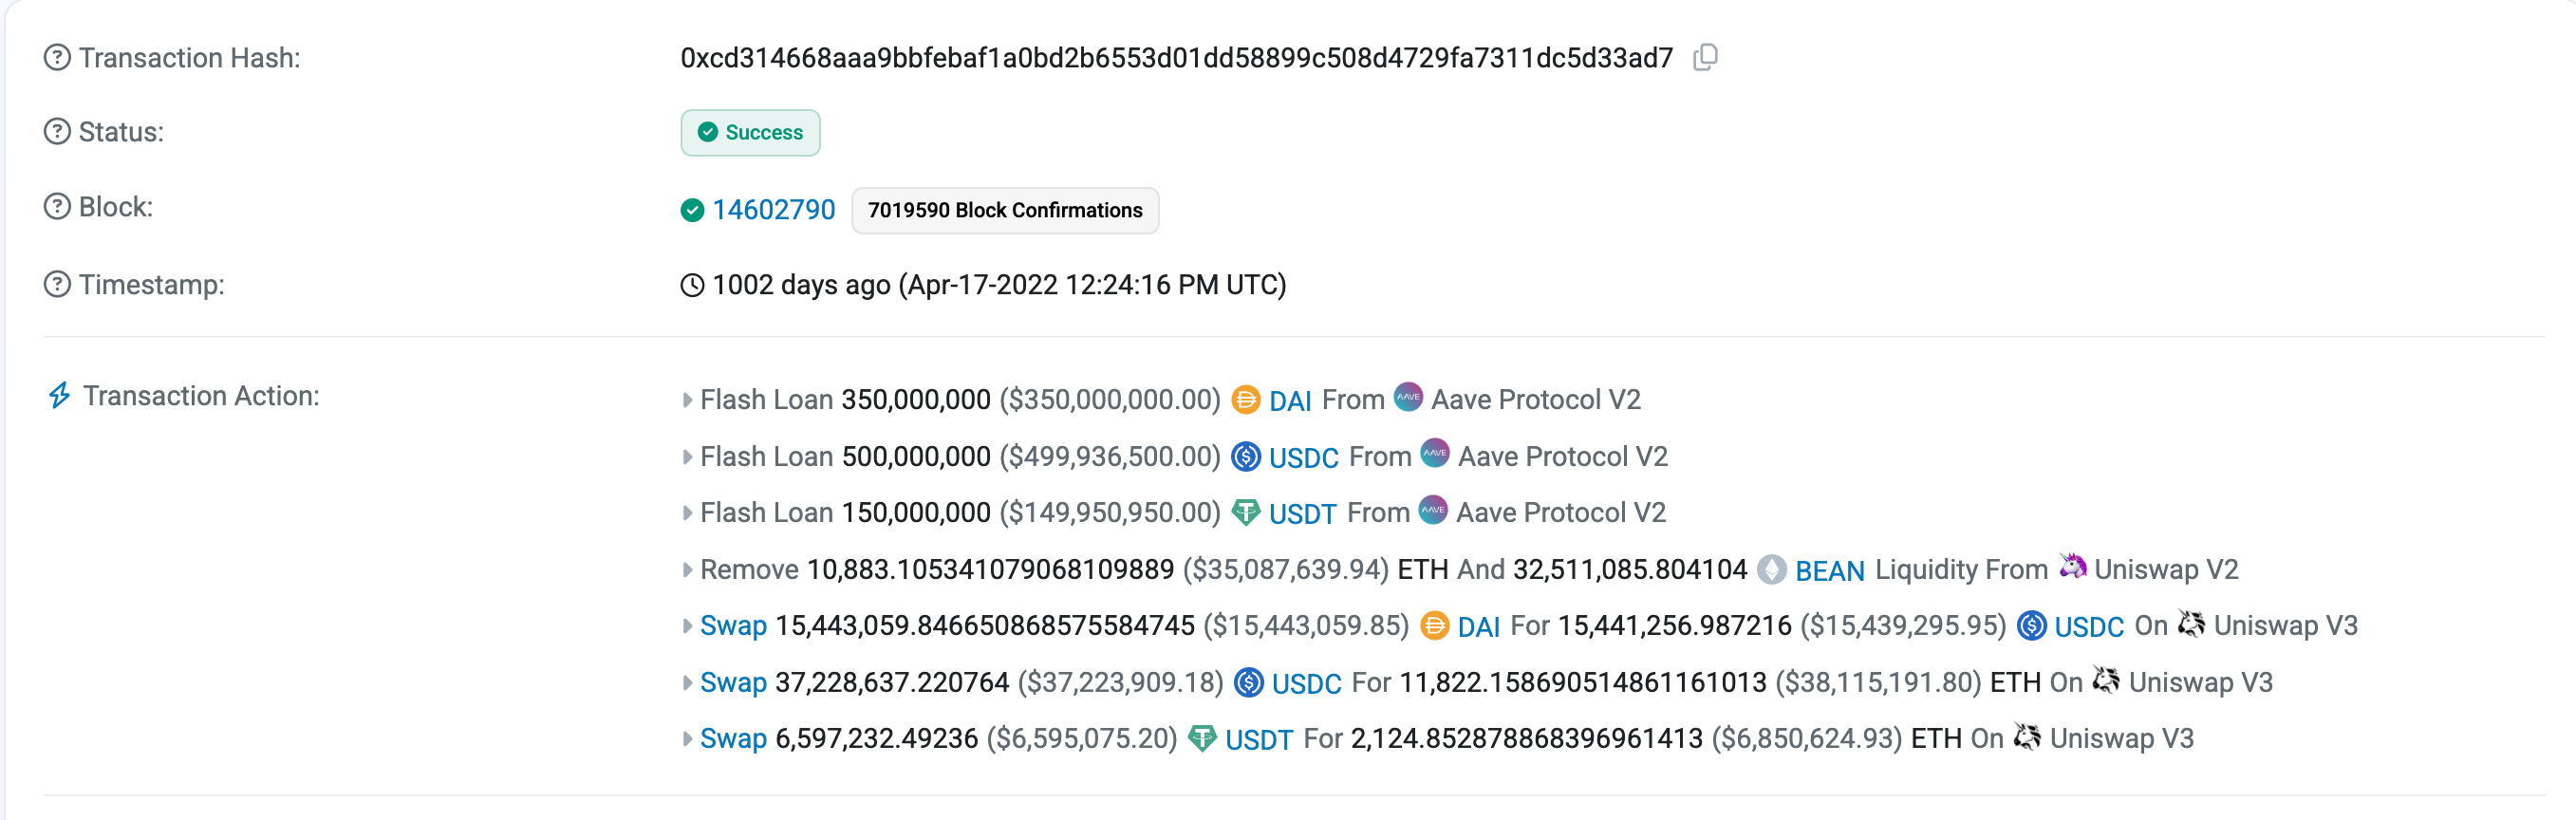
\includegraphics[width=\textwidth, keepaspectratio]{image/beanstalk/etherscan1.png}
    \caption{ Overview of Beanstalk hack.}
    \label{fig:beanstalk1}
\end{figure}
 
 The first observation about the figure \ref{fig:beanstalk1}  is that the transaction has plenty of inner ones, close to 200 which are not displayed for practical reasons, and the real flashloan is the sum of three inner transactions, the top three in the figure,  for a total of 1billion USD (the three stablecoins in the transactions are DAI, USDC, USDT, three very well known flavours of USD in the crypto space). This shows that, from one side using The Graph was very useful to filter out a set of transactions among thousands of flashloans issued, but a full analysis cannot be done just from those data: The Graph subgraph was not designed to consolidate the three inner transactions of the flashloan strongly underestimating the size of the borrowed amount itself. The complexity of the inner transactions is so great that its comprehension has required  to read them in detail.  The tables \ref{tab:beanstalk1}, \ref{tab:beanstalk2} and \ref{tab:beanstalk3} summarise, from a functional point of view, what happened dividing the process in the hack execution, which is the part of the attack directly using the flashloan, including its repayment, the planning of the hack, which consist on a set of transactions done previously after a phase in which beanstalk has been studied in detail by the hacker and  the trade washing, where the hacker, using mixers made impossible to trace the funds he diverted. Mixers, known also as tumblers, are a technology widely used  to obfuscate the orgin and destination of cryptocurrency transactions;  the most famous, tornado cash, is running in the ethereum blockchain and is a decentralised protocols itself.
 
 
 
\begin{table}[H]
\centering
\caption{Hack Execution}
\resizebox{\textwidth}{!}{%
\begin{tabular}{|l|l|}
\hline
\textbf{Action} & \textbf{Details} \\ \hline
\textbf{Initiated flashloan} & Borrowed \$1 billion from Aave to temporarily acquire governance control. \\ \hline
\textbf{Purchased majority BEAN tokens} & Used flashloan funds to buy enough BEAN tokens for a governance majority. \\ \hline
\textbf{Passed and executed proposal} & Drained funds from treasury to attacker-controlled wallets. \\ \hline
\textbf{Repaid flashloan} & Used part of the stolen funds to repay the flashloan within the same transaction. \\ \hline
\end{tabular}%
}
\captionsetup{font=footnotesize, justification=centering}
\caption*{\footnotesize This table summarises the execution phase of the Beanstalk exploit, including the flashloan and proposal execution.}
\label{tab:beanstalk1}
\end{table}


\begin{table}[H]
\centering
\caption{Hack Preparation}
\resizebox{\textwidth}{!}{%
\begin{tabular}{|l|l|}
\hline
\textbf{Action} & \textbf{Details} \\ \hline
\textbf{Deployed malicious proposal} & Submitted a proposal with hidden malicious code to drain funds. \\ \hline
\textbf{Monitored liquidity} & Ensured sufficient BEAN and Aave liquidity for flashloan and execution. \\ \hline
\end{tabular}%
}
\captionsetup{font=footnotesize, justification=centering}
\caption*{\footnotesize This table summarizes the preparation steps for executing the Beanstalk exploit.}
\label{tab:beanstalk2}
\end{table}
 
 
\begin{table}[H]
\centering
\caption{Washing}
\resizebox{\textwidth}{!}{%
\begin{tabular}{|l|l|}
\hline
\textbf{Action} & \textbf{Details} \\ \hline
\textbf{Split stolen funds across wallets} & Distributed the stolen funds across multiple wallets to obfuscate the trail. \\ \hline
\textbf{Utilized mixers and DeFi protocols} & Employed services like Tornado Cash and DeFi platforms to anonymize stolen funds further. \\ \hline
\end{tabular}%
}
\captionsetup{font=footnotesize, justification=centering}
\caption*{\footnotesize This table summarizes the washing phase, where stolen funds were distributed and anonymized.}
\label{tab:beanstalk3}
\end{table}
 
Observing through the inner transactions it is possible to identify, the borrowed money and the interest and principal repayments. This is expected as such inner transactions should always happen or the full transaction would be reverted and not committed to the ethereum. Analysing each of the other transactions is too much detail and the criterion chosen is to explain the main steps of the hack. 


The  complexity of this particular flashloan is  to understand how beanstalk worked at the time of the hack and how the hacker prepared the terrain for the successful usage of a flashloan.


The hacker wallet 0x1c5dcdd006ea78a7e4783f9e6021c32935a10fb4 is the flashloan transactions initializer. Studying it the hack preparation becomes clear. At first the wallet is financed as showed in fig  \ref{fig:beanstalk2} and  \ref{fig:beanstalk3}.
\begin{figure}[ht]
    \centering % Properly centers the image
    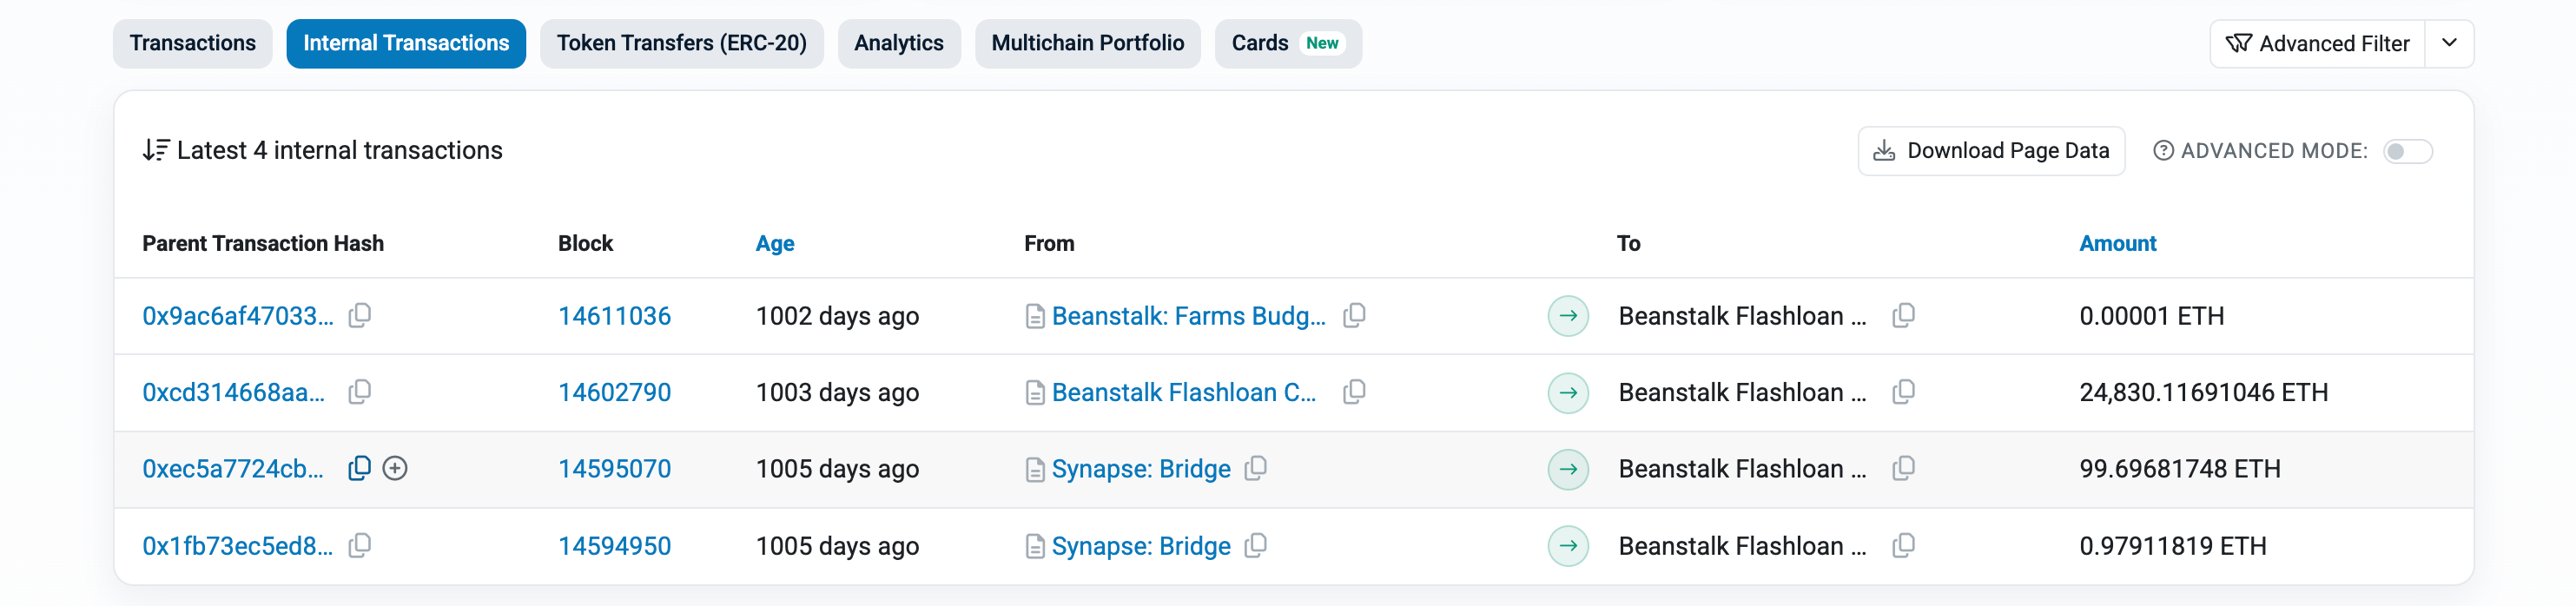
\includegraphics[width=\textwidth, keepaspectratio]{image/beanstalk/etherscan_fin_wallet.png}
    \caption{Overview of hacker wallet financing through synapse}
    \label{fig:beanstalk2}
\end{figure}


\begin{figure}[ht]
    \centering % Properly centers the image
    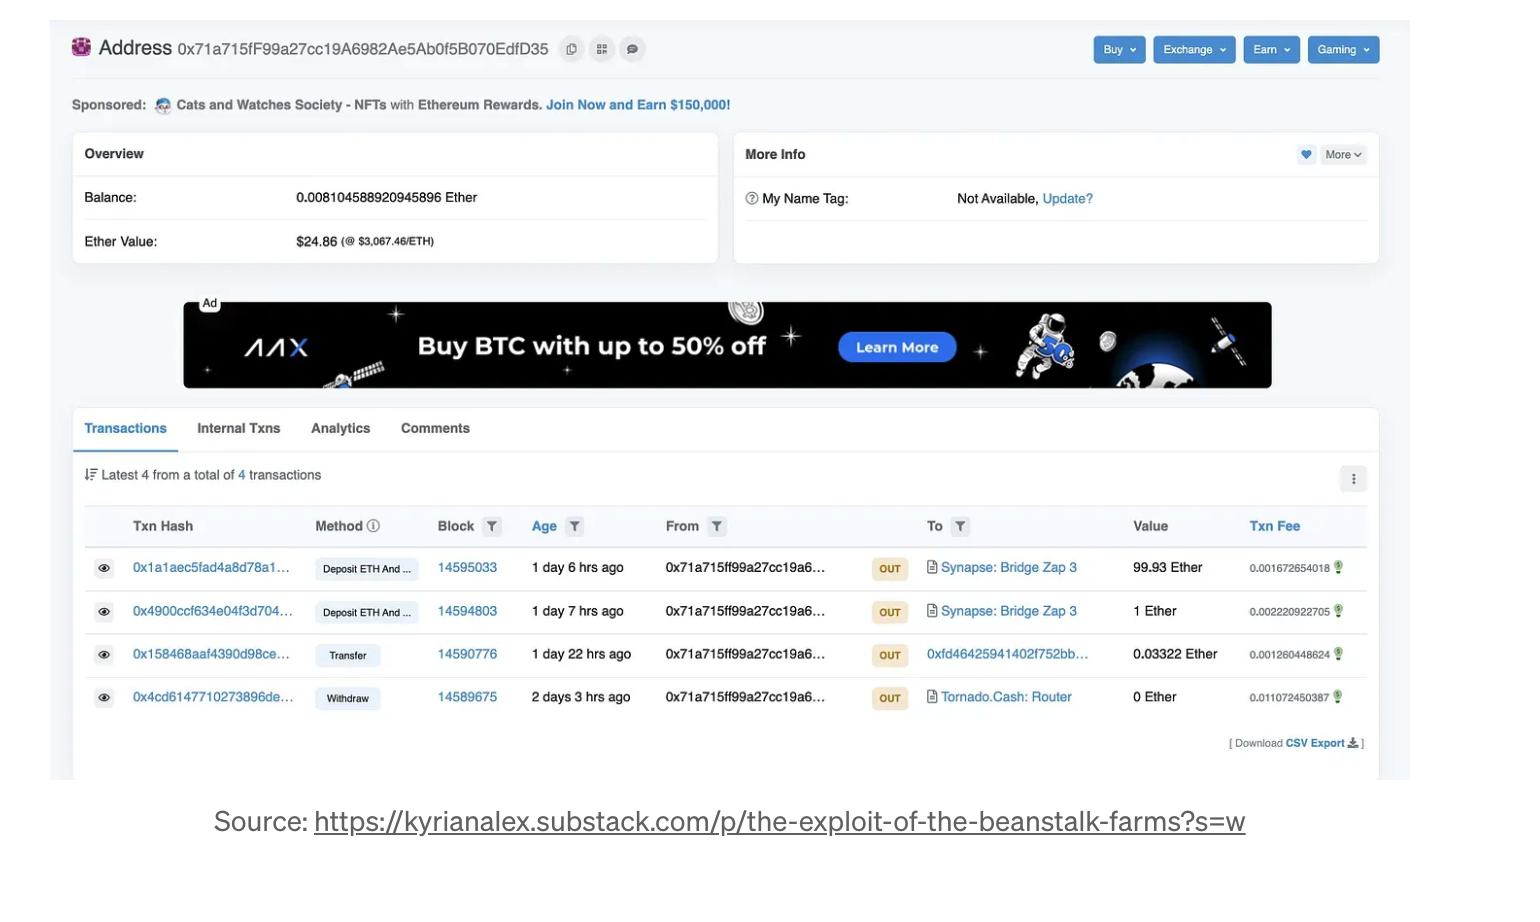
\includegraphics[width=\textwidth, keepaspectratio]{image/beanstalk/hackerfinancingWallet.png}
    \caption{Overview of Synapse and other tools preloaded }
    \caption*{\footnotesize \textit{Source: \url{https://medium.com/@nvy_0x/the-beanstalk-bean-exploit-b038f4d324ea}}}
    \label{fig:beanstalk3}
\end{figure}





The hacker knows very deeply the protocol governance, including its flaws and how to write sophisticated smart contracts by leveraging well tested libraries to use hidden features of the EVM.
In the specific case: Beanstalk is a DAO with a governance which is based on majority vote. Such vote can be exercised by staking BEAN tokens or staking LP (liquidity pools). A security implementation of the protocols happens to become the exploitetd flaw: to defend the DAO from hacks, the protocol allows to trigger emergency proposal with the 2/3rds of voting power by allowing the the approval of a proposal with just 24 hours delay from its presentation by triggering a code called emergencyCommit().



 Obviously the protocol implementors always check if a proposal is malicious by processing it in advance and it looks reasonable that nobody will perform an attack out of nowhere in an ethereum transaction.
 
 
 \begin{figure}[ht]
    \centering % Properly centers the image
    \includegraphics[width=\textwidth, keepaspectratio]{image/beanstalk/maliciousProposalExecution.png}
    \caption{malicious proposal execution.}
    \label{fig:proposalexec}
\end{figure}
 
 \begin{figure}[ht]
    \centering % Properly centers the image
    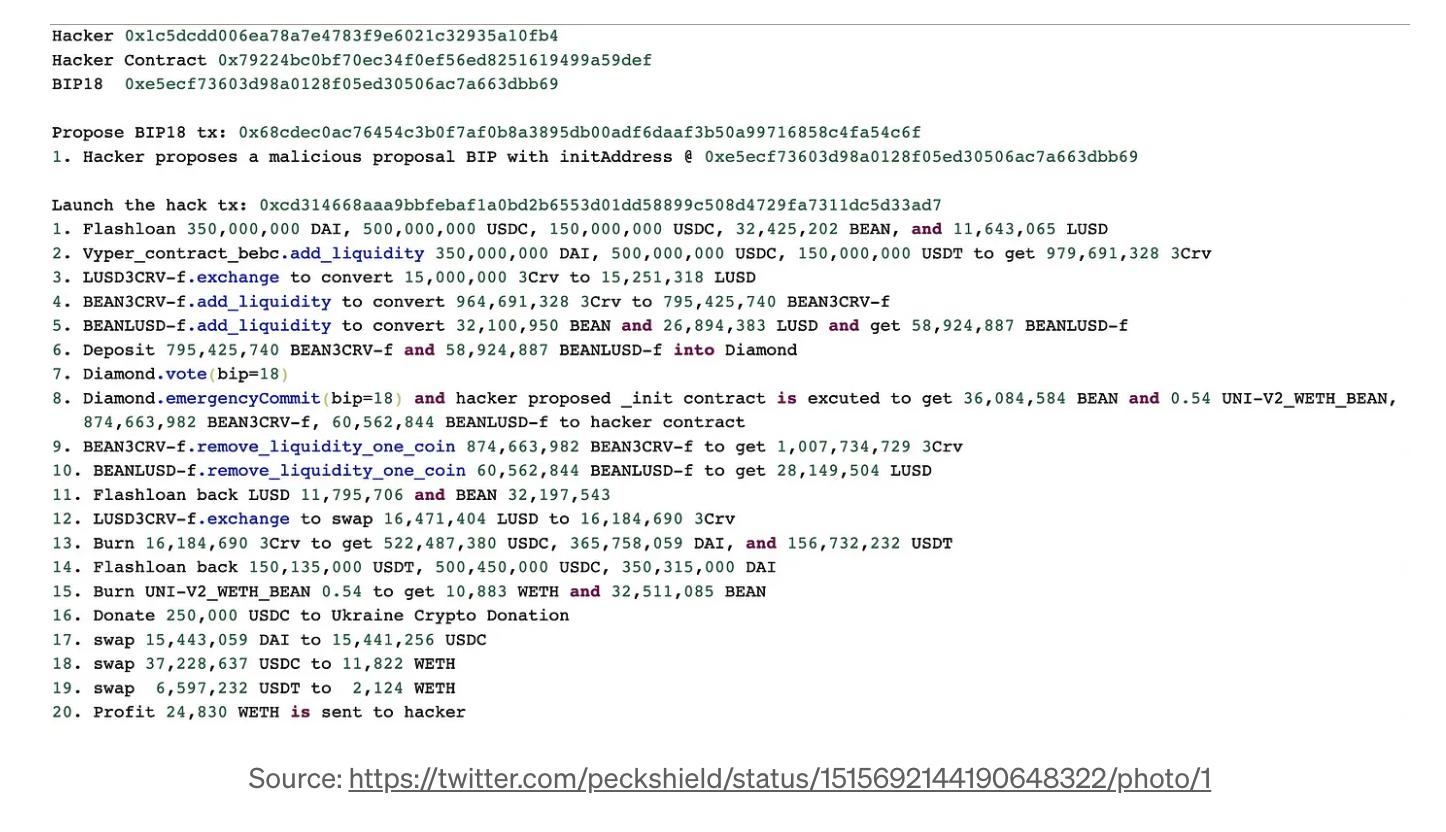
\includegraphics[width=\textwidth, keepaspectratio]{image/beanstalk/divertingfunds}
    \caption{diverting funds.}
    \label{fig:divfunds}
\end{figure}

 
 
 The idea is that a proposal is  submitted and voted at large majority if the protocol looks under attack. Here comes the smart hacker with the second step in the hack preparation: two proposals are submitted 1 day (24 hours) before the flashloan appearently not correlated. In reality one,classified as a proposal to donate fund to Ukraine, allows a smart contract to be deployed to a precomputed address: reverse engineering the code in such address, which is available on chain, it is clear that the address contains a malicious code, which exploiting a bug in the beanstalk protocol executed the emergencyCommit() and  sends all the treasury reasources to itself. The second contract created by the hacker is very likely a kind of spam to obfuscate the malicious one: it is not directly involved in the process.
 The triggering of the malicious proposal is rendered in figure \ref{fig:proposalexec}



With all these steps in place the hacker, during the flashloan has only to reach the 2/3rd majority by adding the missing voting power which he buys with the borrowed money, then trigger the call to the malicious contract which will clear all the funds sending them to his wallet.
This wallet 0x1c5dcdd006ea78a7e4783f9e6021c32935a10fb4 sends afterwards hundreds of transaction of 100 ethers to mixers washing the money which is delivered to many unknown and hardly identifiable addresses.
The fund diversion is rendered in the figure \ref{fig:divfunds}






The described hack is one of the biggest ever happened. Differently from many, for example the Euler protocol hack, also performed through an Aave V2 flashloan, the distracted funds have never been returned.
After this experience governance protocols have included a delay time between the call and  execution of a protocol smart contract as a protection against malicious usage of flashloans.
The measures generally suggested to avoid a DAO hack are summarised in the table \ref{tab:flashloan_mitigation}

\begin{table}[H]
\centering
\caption{Mitigation Strategies for Flashloan Attacks}
\resizebox{\textwidth}{!}{%
\begin{tabular}{|l|p{0.8\textwidth}|}
\hline
\textbf{Strategy} & \textbf{Description} \\ \hline

\textbf{Time-weighted Governance} & 
Require governance votes to be based on token holdings over time, reducing the ability of attackers to temporarily acquire voting power through flashloans. \\ \hline

\textbf{Proposal Review Period} & 
Introduce a delay between proposal submission and execution to allow the community to detect and address malicious proposals. \\ \hline

\textbf{Governance Token Staking} & 
Mandate staking of governance tokens for a fixed period before they can be used for voting, preventing instant use of flashloan-acquired tokens. \\ \hline

\textbf{Flashloan-resistant Logic} & 
Implement transaction logic that ignores changes in token balances occurring within a single block to invalidate flashloan-based manipulations. \\ \hline

\textbf{Limits on Single Transactions} & 
Enforce limits on the maximum amount of funds or tokens that can be moved in a single transaction to minimize the damage from exploitative actions. \\ \hline

\textbf{Decentralized Audits} & 
Regularly conduct audits and simulations to test for vulnerabilities, including governance-related exploits and flashloan attacks. \\ \hline

\textbf{Oracle Manipulation Defense} & 
Use robust and decentralized oracles to prevent attackers from influencing on-chain price feeds during flashloan attacks. \\ \hline

\textbf{Risk Flagging Systems} & 
Deploy automated monitoring tools to detect unusual transactions or flashloan patterns, triggering alerts for further investigation. \\ \hline

\textbf{Community-driven Governance} & 
Empower diverse stakeholders in governance, reducing the influence of temporary, centralized token holdings acquired through flashloans. \\ \hline

\textbf{Hard-coded Safety Mechanisms} & 
Embed hard limits on treasury withdrawals or critical operations, requiring multi-sig or multi-stage approvals for large or unusual transactions. \\ \hline

\end{tabular}%
}
\captionsetup{font=footnotesize, justification=centering}
\caption*{\footnotesize This table highlights strategies that protocols can adopt to mitigate flashloan-related vulnerabilities, inspired by lessons learned from the Beanstalk exploit.}
\label{tab:flashloan_mitigation}
\end{table} 
 
\subsection{Flashloan for pseudo arbitrage on incentives}

The transaction 0x7567551456d5bafc6816e40b3dfa27de4040d140430c7d815e641d301755fb0b and 0xa55285d2d43562befbc4d2e76e722f4e34973a42cfe9f40b5222bf0f68bb8841 are the second and third greatest flashloan ever issued in Aave V2 ethereum. They are both issued by the same wallet and the mechanic is identical, therefore it is enough to document one. \\
 The transaction 0x7567551456d5bafc6816e40b3dfa27de4040d140430c7d815e641d301755fb0b is much more simple than the protocol hack seen previously but it is complex to understand how the setup of a profitable trade has been achieved. The main challenge is find a meaning for the full inner transactions which looks at a first glance not profitable and therefore illogical. All the inner transactions are just eight and are rendered in the figure   \ref{fig:humphy1} 

\begin{figure}[ht]
    \centering % Properly centers the image
    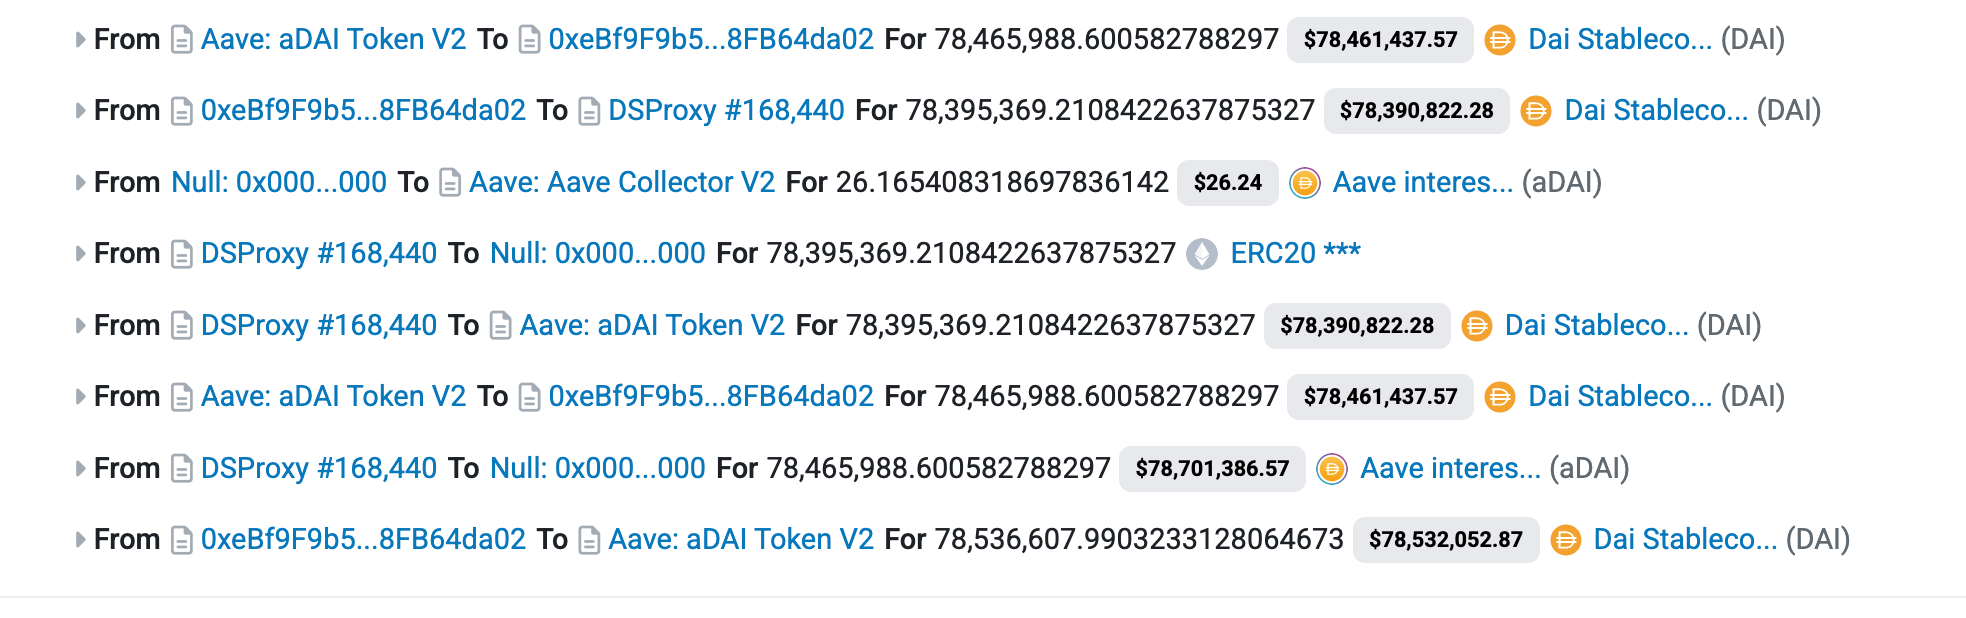
\includegraphics[width=\textwidth, keepaspectratio]{image/humpyDSProxy/innerTxHumphy.png}
    \caption{Etherscan overview of DSProxy call within a flashloan.}
    \label{fig:humphy1}
\end{figure}

The choice of displaying an etherscan view is  dictated by the mapping of wallet to known names, in this case Humpy, an extremely active multichain crypto whale making large usage of DEFI tools with advanced  development skills and DSProxy, a very important tool to execute bolckchain  code within a transaction.
To understand what happened and how Humphy profited from the flashloan the inner transactions cannot be of any help: actually etherscan doesn't even render properly the amounts as can be noted by looking the flashloan repayment amount. For this paper scope has been necessary to proceed to a deep analysis of the logs emitted by the transactions and the smart contract called. They are available in the erigon node, and accessible through otterscan, but etherscan though less complete allows to map easier the names, therefore the figures will refer to etherscan for ease of usage.
From the inner transactions and the logs a set of interacting protocols and tool are clearly identified: Aave, DSProxy, Humpy. Aave has been already described and Humpy is just the logical name of a wallet, DSProxy, instead, plays a very important role in the current transaction and requires some additional note. Calling a protocol, for example Aave, to execute complex operations requires to operate programmatically deploying one or more smart contracts on the blockchain; this expose directly the wallet of the contracts creator and can become complicate. Additionally, a common scenario, is calling different protocols in a unique transaction and DSProxy addresses  this natively. The protocol is well tested and used behind the scenes by very famous DEFI  protocols, in particular MakerDAO, the protocol behind the first DEFI stablecoin, DAI, which was created as a stablecon  pegged to USD and collateralised by eth and has evolved to a multicollateralised stablecoin with the operation to swap  collaterals handled transparently through DSProxy.

\begin{table}[H]
\centering
\caption{DSProxy Functionality Summary}
\resizebox{\textwidth}{!}{%
\begin{tabular}{|l|l|}
\hline
\textbf{Functionality} & \textbf{Description} \\ \hline
\textbf{Proxy for User Interactions} & Acts as a smart contract proxy to allow users to interact with DeFi protocols on their behalf. \\ \hline
\textbf{Execute Calls} & Executes arbitrary calls on behalf of the user, enabling complex interactions. \\ \hline
\textbf{Access Control and Security} & Provides security by allowing users to delegate specific actions to the proxy, instead of exposing their funds directly. \\ \hline
\end{tabular}%
}
\captionsetup{font=footnotesize, justification=centering}
\caption*{\footnotesize This table summarizes the key functionalities of the DSProxy contract, used for interacting with DeFi protocols securely and efficiently.}
\label{tab:dsproxy_functionality}
\end{table}


\begin{figure}[ht]
    \centering % Properly centers the image
    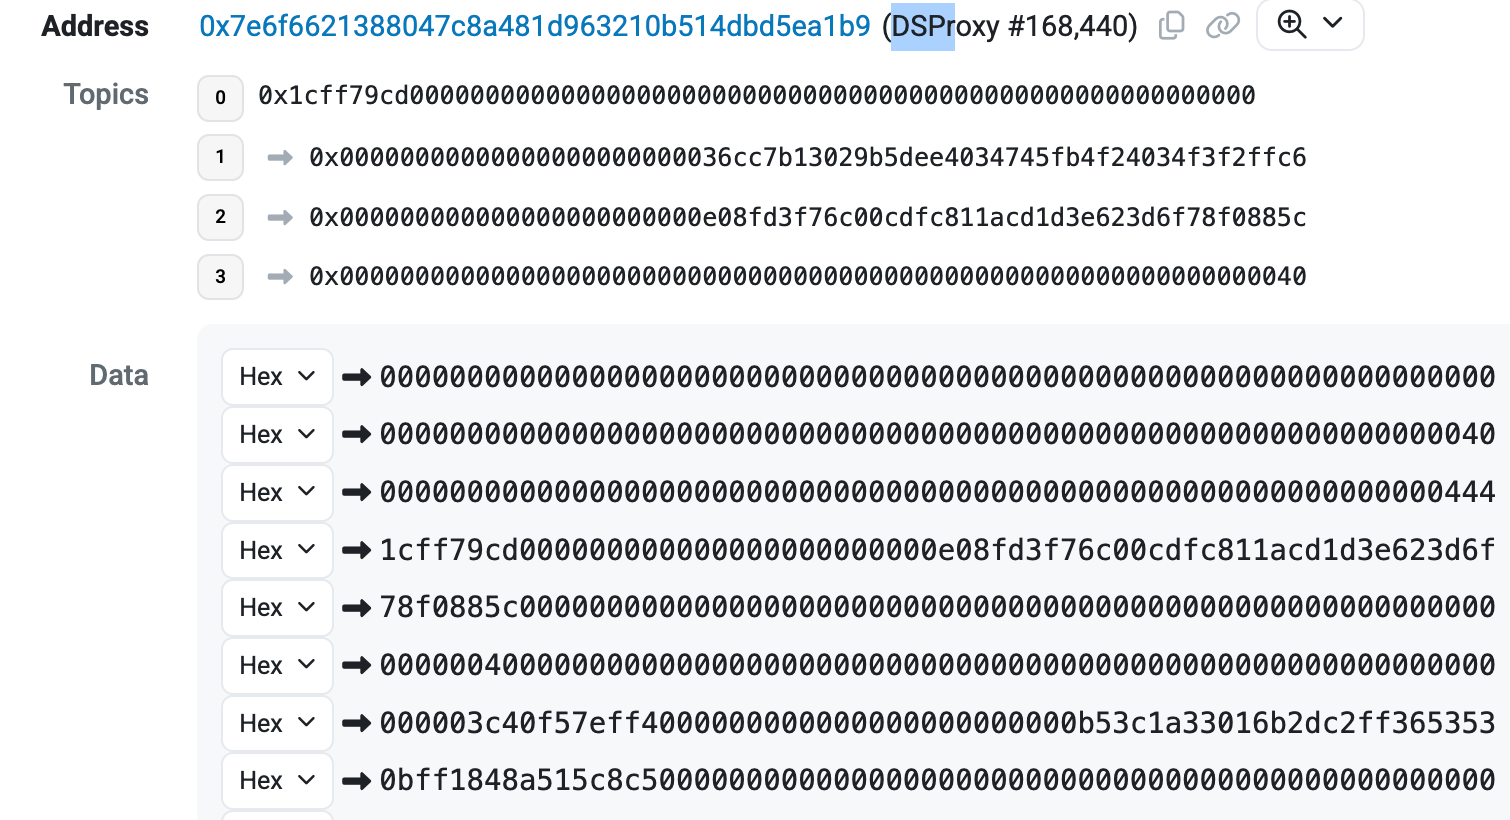
\includegraphics[width=\textwidth, keepaspectratio]{image/humpyDSProxy/innerlog.png}
    \caption{Excerpt of an inner log}
    \label{fig:humphy2}
\end{figure}

By observing the most meaningful emitted logs, in \ref{fig:humphy2} an example of what has been used for the analysis,  DSProxy is called twice redirecting the end result of its inner transactions to the humphy wallet and calling two smart contracts of the Aave protocol other than the flashloan ones:  Incentives Controller with rewardsAccrued  and AaveSaverTakerOV2.
The  reason is that Aave V2 protocol was running an incentive program at that time, rewarding certain kind of usage with native tokens: Humpy likely used this opportunity to perform a set of operations in the protocol and get such incentives.
 No investigations are done about possible  subtle interactions with pre-existing positions (e.g., adding liquidity briefly, leveraging yield mechanics which are  plausible but extremely hard to trace).
 
The best comparison with traditional finance is a regulatory arbitrage in this case performed exploiting a reward mechanism.




\subsection{Flashloan for obfuscating a transaction }

The transaction 0x04c43669c930a82f9f6fb31757c722e2c9cb4305eaa16baafce378aa1c09e98e returned as the fifth biggest flashloan ever in Aave V2.0 correspondent to 38,100,000 DAI. 
The transaction includes a flashloan and  a very big swap

\begin{figure}[ht]
    \centering % Properly centers the image
    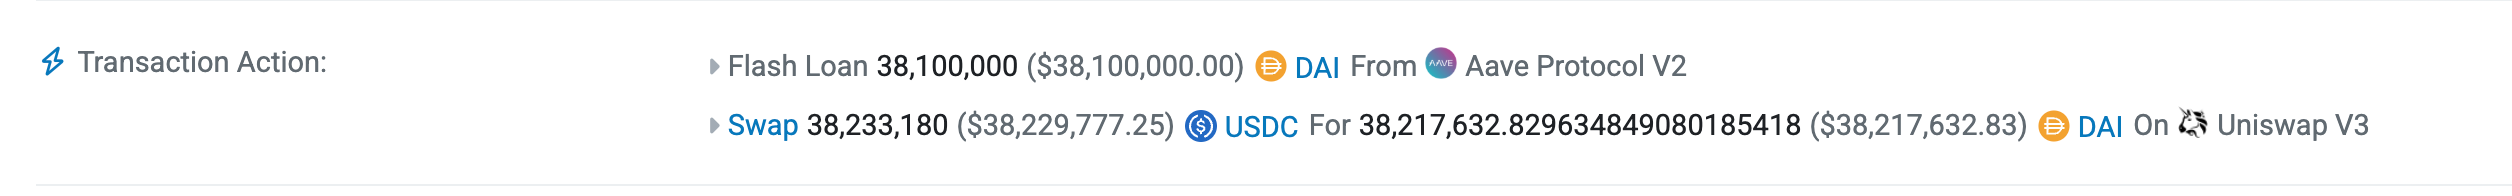
\includegraphics[width=\textwidth, keepaspectratio]{image/boshen/boshen1.png}
    \caption{Overview of main transactions.}
    \label{fig:boshen1}
\end{figure}


\begin{figure}[ht]
    \centering % Properly centers the image
    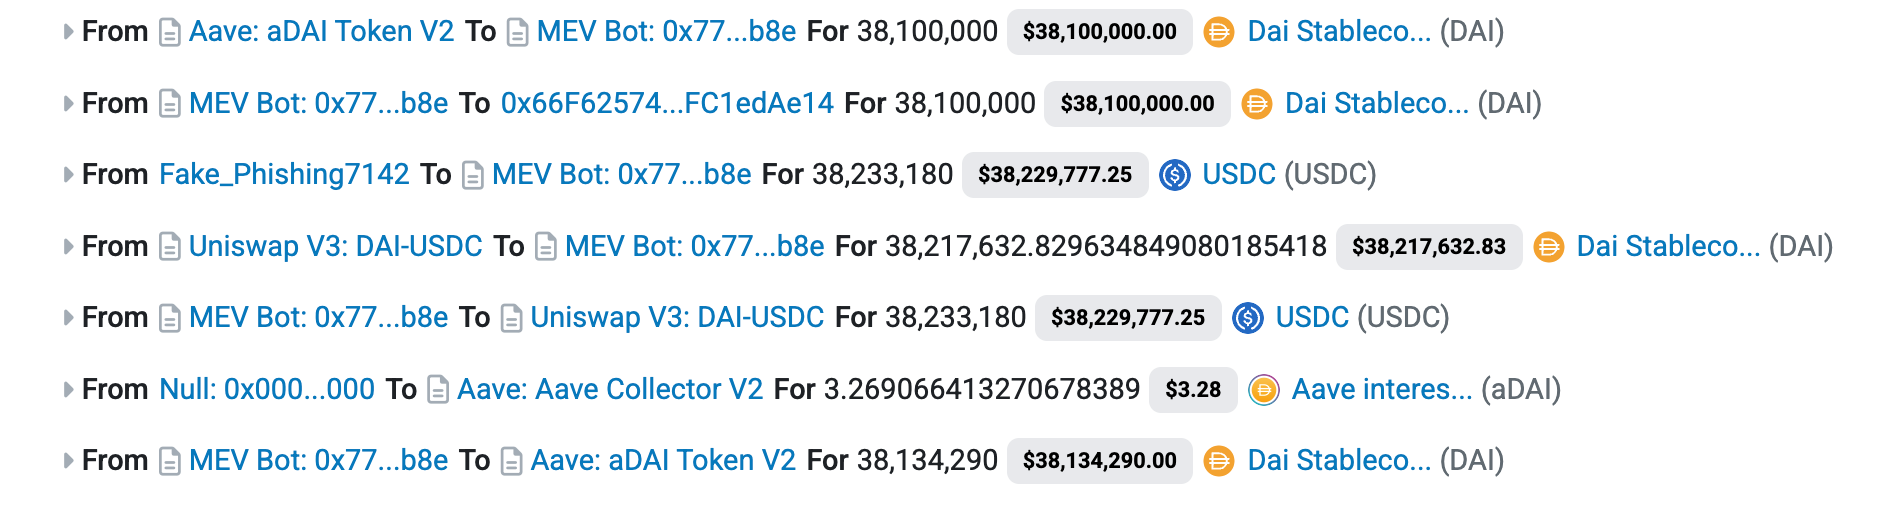
\includegraphics[width=\textwidth, keepaspectratio]{image/boshen/boshen2.png}
    \caption{Overview of inner flashloan transactions.}
    \label{fig:boshen2}
\end{figure}

\begin{figure}[ht]
    \centering % Properly centers the image
    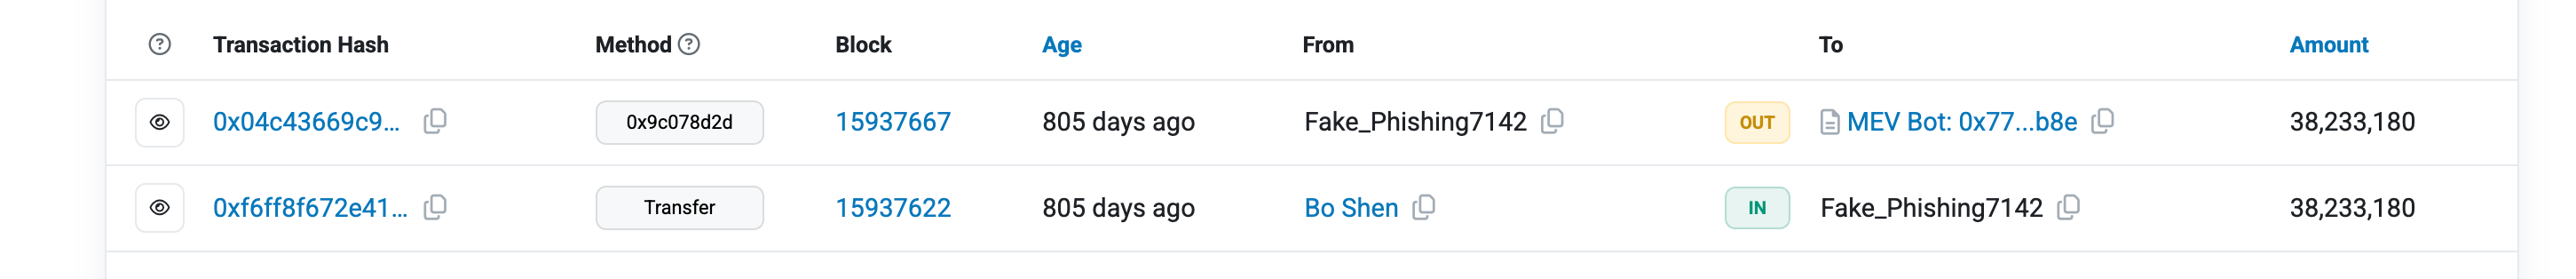
\includegraphics[width=\textwidth, keepaspectratio]{image/boshen/boshen3.png}
    \caption{wallet owning the initial funds}
    \label{fig:boshen3}
\end{figure}


The figure \ref{fig:boshen1} shows the main transactions, a 38,100,000 DAI flashloan and the swap, realised in uniswap of 38,233,180 USDC in 38,217,632 DAI
The swap, although very big is only influencing minimally the price of DAI generating a little loss. In parallel a flashloan is issued as showed in figure  \ref{fig:boshen2}.
The same figure shows the repayment of the flashloan including the premium.
The analysis of the inner transactions shows a very irrational behaviour as the original fund could have simply been converted to DAI. The flashloan itself adds a premium paid in addition to the normal usage of uniswap, making the trade expensive in every component of it. In the previous cases was possible to see flashloans expensive in terms of premium paid but the end result of the transaction was a gain, basically from protocol hack or a meaningful action as a collateral swap and, in general, the common use, not necessarily related to interesting transactions, is using the flashloan to support another action. In this the flashloan is not different from a normal loan. The anomaly that has to be explained is why has the flashloan been called at all in this case. Observing figure  \ref{fig:boshen3}   the wallet owning the initial funds (the choice not to render the wallet id but labels helps in connecting the dots) is displayed as belonging to Bo Shen a famous crypto investor funding parter of the asian crypto fund Fenbushi capital and performs a transaction to Fake\_Phishing\_7142 of 38,233,180 USDC, which, first line of the figure performs one of the inner transactions of the flashloan from  \ref{fig:boshen2}, the swap of USDC to DAI is the inner transaction performed immediately  afterwards. Bo Shen notified  the stealing of the private key of one of his wallets containing BTC, Usdc and other cryptos. What happened is now totally consistent: Switching to DAI move from a usd stablecoin handled by a centralized authority, USDC, to one fully decentralised, performing the operation within a flashloan has the additional benefit of concealing the connection between the stolen wallet and the swap itself.

\begin{table}[H]
\centering
\caption{Summary of Flashloan Caller Actions and Analysis}
\resizebox{\textwidth}{!}{%
\begin{tabular}{|l|p{0.8\textwidth}|}
\hline
\textbf{Steps} & \textbf{Summary} \\ \hline
\textbf{Identification of Anomalous Behavior} & 
The flashloan caller utilized a flashloan unnecessarily, incurring additional premium costs without achieving any visible profit \\ \hline

\textbf{Result of Additional Analysis} & 
A wallet attributed to Bo Shen (a notable crypto investor and Fenbushi Capital partner) is connected through a transaction with another wallet involved  in the flashloan \\ \hline

\textbf{Incident Report} & 
Bo Shen publicly disclosed that one of his wallet's private keys had been stolen. \\ \hline

\textbf{Rationale Behind the Flashloan and Swap} & 
The flashloan caller converted USDC (a centralized stablecoin) to DAI (a decentralized stablecoin) to avoid the risk of USDC being frozen by its issuer, Circle. Using a flashloan to execute the swap helped obscure the link between the stolen wallet and the asset conversion, adding complexity to the transaction trail. \\ \hline

\textbf{Final Assessment} & 
The flashloan caller did not use the flashloan to generate profit but rather to mask the origins of the stolen funds and secure them in a decentralized, unfreezable form (DAI). \\ \hline
\end{tabular}%
}
\captionsetup{font=footnotesize, justification=centering}
\caption*{\footnotesize This table outlines the steps and analysis of the flashloan caller's actions, highlighting the rationale and implications behind the transactions.}
\label{tab:flashloan_analysis}
\end{table}



\subsection{Flashloan call for MEV (front running trades)}





\subsection{Flashloan call for arbitrage (find a real arbitrage)}

\newpage



\section{Literaturverzeichnis}
Gantenbein, Pascal, und Marco Gehrig, 2007, Moderne Unternehmensbewertung, \textit{Der
Schweizer Treuhänder}, S. 602 – 612.


\newpage
\section{Anhang}
\subsection*{Eidesstattliche Erklärung}
Hiermit erkläre ich, dass ich die vorliegende Arbeit selbständig und ohne Benutzung anderer als der angegebenen Hilfsmittel angefertigt habe. Mir ist bekannt, dass ich die volle Verantwortung für die Wissenschaftlichkeit des vorgelegten Textes selbst übernehme, auch wenn KI-Hilfsmittel eingesetzt und deklariert wurden. Alle Stellen, die wörtlich oder sinngemäss aus veröffentlichten oder nicht veröffentlichten Schriften entnommen wurden, sind als solche kenntlich gemacht. Die Arbeit ist in gleicher oder ähnlicher Form oder auszugsweise im Rahmen einer anderen Prüfung noch nicht vorgelegt worden.\\
\noindent Ort, den XX.XX.20YY
\begin{flushright}
$\overline{~~~~~~~~~\mbox{(Unterschrift der Verfasserin)}~~~~~~~~~}$
\end{flushright}

\end{document}  



